\documentclass[12pt,a4paper,oneside,openright]{Tptesi2}
%\documentclass[a4paper,oneside]{Tptesi2}

 % needed for \Set

\usepackage[american]{babel}

\usepackage{amsmath,amssymb}
\DeclareMathOperator*{\argmin}{argmin} 

\usepackage{acronym}
\usepackage{multicol}
\usepackage{verbatim}
\usepackage{indentfirst}
\usepackage[utf8]{inputenc}  
\usepackage{algorithm}
\usepackage[noend]{algpseudocode}
\usepackage{subfigure}
\usepackage{framed}
\usepackage{rotating}
\usepackage{listings}
\usepackage{graphicx}
\graphicspath{ {img/} }
\usepackage{wrapfig}
\usepackage{matlab-prettifier}
\usepackage{enumitem}
\usepackage{hyperref}
\setlist{nosep}
%\usepackage{pdf14}
\usepackage[font=small]{caption}
\usepackage{booktabs}


\acrodef{BS}{base station}
\acrodef{DL}{downlink}
\acrodef{DTX}{discontinuous transmission}
\acrodef{EC}{energy consumption}
\acrodef{EE}{energy efficiency}
\acrodef{ICT}{information and communication technology}
\acrodef{ML}{machine learning}
\acrodef{OPEX}{operational expenditure}
\acrodef{PA}{power amplifier}
\acrodef{PAR}{peak-to-average ratio}
\acrodef{QoS}{quality-of-service}
\acrodef{RB}{resource block}
\acrodef{RE}{resource element}
\acrodef{RL}{reinforcement learning}
\acrodef{SM}{sleep mode}
\acrodef{TD}{temporal difference}
\acrodef{UE}{user equipment}
\acrodef{UL}{uplink}



\interfootnotelinepenalty=10000 % prevent footnotes from going into an other page.

\usepackage[hyperref=true,
url=false,
isbn=false,
style=numeric-comp,
citereset=chapter,
maxcitenames=3,
maxbibnames=100,
block=none]{biblatex}

% Use a small font for the verbatim environment

\makeatletter  % makes '@' an ordinary character
\renewcommand{\verbatim@font}{%
	\ttfamily\footnotesize\catcode`\<=\active\catcode`\>=\active%
}

\makeatother   % makes '@' a special symbol again

\DeclareMathOperator*{\argmax}{arg\,max}


\hypersetup{%
	pdfstartview= {XYZ null null 1.00},%
	plainpages=false,%
	breaklinks,%
	pdftitle={Effective sleep mode management by means of reinforcement learning for LTE cellular networks},%
	pdfauthor={Daniele Giacomelli},%
	pdfsubject={Tesi Magistrale},%
	pdfkeywords={Base Station, Machine Learning, Reinforcement Learning, Energy Efficiency, SARSA algorithm, Green Network},%
	colorlinks=false}
\bibliography{Bibliografia}


% Formattazione Figure -----------------------------------------------------------
\setcounter{topnumber}{3}
\setcounter{totalnumber}{3}
\def\topfraction{1}
\def\textfraction{0}
% Fuzz ---------------------------------------------------------------------------
%\hfuzz10cm %Non scassare linee che escono dal bordo
% Frontespizio -------------------------------------------------------------------
       \title{Data-driven Birdstrike Risk Estimation}
       \author{Alessandro Minervini}
       \titolocorso{Ingegneria Informatica}
       \chair{Prof. Andrew D. Bagdanov}
       \othermembers{Prof. Fabio Schoen}
       \numberofmembers{2} %numero dei relatori
       
       \degreeyear{2018/19}
       \numerocorrelatori{1} %numero dei correlatori
       \correlatori{Ing. Walter Nunziati} % i correlatori separati da \\

%
% ---- Inclusioni (vedi piu` sotto per il comando "include" --------------
%\includeonly {introduzione,chapter1, chapter2}
%\includeonly {chapter1, chapter2, chapter3, chapter4, chapter5, chapter6}
%\includeonly{chapter6}
%


\begin{document}

\frontmatter

%\hyphenation{}
%
\pagestyle{headings} % rende attive le impostazioni sulla testata!
%
\maketitle % crea il frontespizio (ricordati di copiare "stemma.eps" nella tua 
%%directory)
%
%

\pagenumbering{roman}
\chapter*{Abstract}
Wildlife strike events (or more commonly, birdstrikes) are a dangerous and growing phenomenon due to the increase in flights over the years. Unfortunately, airports are attractive places for birds and other animals which can cause serious wildlife strike accidents.

This phenomenon can be seriously dangerous for the safety of passengers and very expensive for civil aviation, not only in Italy, to sustain the cost of prevention, repair and delays caused.
To keep airports safe it becomes very important to prevent these events.

At the moment in all Italian airports the Birdstrike Risk Index version 2.0 ($BRI_2$) is used to monitor risk of wildlife strike events. It provides a monthly value that identifies the risk to which each airport is subject. 

We conducted an in-depth analysis of $BRI_2$ to estimate the quality of this risk index, its correlation with historically occurring wildlife strike events, in order to understand if it is a good tool for measuring actual wildlife risk.
Some limitations of the $BRI_2$ have been found. A risk-index for this phenomenon must show a relevant correlation with wildlife strike events. 

In this thesis we develop a data-driven model for wildlife strike risk estimation. Our approach is based on a Recurrent Neural Network (RNN) trained to predict a wildlife strike risk estimate that is as correlate as possible with historically occurring wildlife strike events in many Italian Airports, on the basis of a fifteen-day window of data.
Our evaluation, using data from a subset of eight different airports, show encouraging results achieved by our approach demonstrating the superior predictive quality of our model with respect to $BRI_2$.
\chapter*{Sommario}

Gli eventi wildlife strike (o più comunemente birdstrike) sono un pericoloso fenomeno in crescita a causa dell'aumento dei voli aerei nel corso degli anni. Gli aeroporti sono purtroppo luoghi attrattivi per uccelli ed altri animali i quali possono provocare incidenti di wildlife strike anche di seria entità.
Questo fenomeno può essere seriamente pericoloso per la sicurezza dei passeggeri e molto costoso per l'aviazione civile, non solo italiana, sostenere i costi di prevenzione, di riparazione e per i ritardi provocati.
Per mantenere gli aeroporti sicuri diventa molto importante prevenire questi eventi.

Al momento in tutti gli aeroporti italiani per monitorare il rischio di wildlife strike è utilizzato il Birdstrike Risk Index version 2.0 ($BRI_2$). Esso fornisce un valore mensile che identifica il rischio a cui è soggetto ogni aeroporto. 
Un'analisi profonda è stata condotta sul $BRI_2$ stimando la qualità di questo indice di rischio, e la correlazione con gli eventi di wildlife strike storicamente accaduti, per capire se è un buon strumento capace di riconoscere i periodi di maggiore pericolosità di questo fenomeno.
Alcune limitazioni del $BRI_2$ sono state rilevate. Un indice di rischio per questo fenomeno deve manifestare una rilevante correlazione con gli eventi di wildlife strike.

In questa tesi è stato sviluppato un modello data-driven per la stima del rischio degli eventi di wildlife strike. Il nostro approccio è basato su una Recurrent Neural Network (RNN) allenata a predirre una stima del rischio di wildlife strike che sia il più correlato possibile con gli eventi di wildlife storicamente accaduti sulla base di una finestra di osservazioni di 15 giorni.
La nostra valutazione, usando dati provenienti da otto diversi aeroporti, mostrano risultati incoraggianti raggiunti dal nostro approccio, dimostrando la superiore qualità predittiva del nostro modello rispetto al $BRI_2$.
\chapter*{Acknowledgements}

I would like to express my gratitude to BirdControl Italy S.r.l., owner of the BirdControl DBMS database, containing the data of 10+ years of monitoring activities in several Italian airports, used for this thesis.
The BirdControl DBMS database has been of fundamental importance for the $BRI_2$ analysis and for the development and testing of the proposed data-driven model. 
I am also grateful to Magenta s.r.l. and Prof. Andrew D. Bagdanov for the opportunity given, for the workspaces and for the consultancy provided.
Finally, i wish to thank my family and friends for their support and in particular my university colleagues for their enthusiastic encouragement and useful critiques of this thesis work.


\tableofcontents % inserisce indice generale
\cleardoublepage
%\addcontentsline{toc}{chapter}{Elenco delle figure}
%\listoffigures   % inserisce indice figure
%\addcontentsline{toc}{chapter}{Elenco delle tabelle}
%\listoftables    % inserisce indice tabelle
%\addcontentsline{toc}{chapter}{Elenco degli algoritmi}
%\listofalgorithms
%
%--------------- Inizio del testo vero e proprio
%

%\cleardoublepage
%\pagenumbering{arabic}
\include{files/ringraziamenti}

\mainmatter
\chapter{Introduction}\label{ch:Ch.1}

Wildlife strike generally means the violent impact between an aircraft and one or more wild animals, mainly birds (birdstrike), with more or less relevant consequences, depending on the size and number of animals impacted, the flight phase and the part of the aircraft that is hit.
Bird strikes occur most frequently during take-off or landing (about 90\% of cases) and on low-altitude flights. However, cases of impact with birds have also occurred at higher elevations, such as 6 000 or 9 000 meters above sea level \cite{wikipedia_it}.

The damage caused is considerable. Since 1910 there have been 350 military deaths and 250 civilian deaths due to impact with birds and moreover the wildlife strike is constantly increasing all over the world \cite{wikipedia_it}. This is mainly due to the progressive increase in air traffic, the mandatory reporting and the higher attention to the problem.

Some relevant cases have happened. Just a year ago on August 15, 2019, Ural Airlines Flight 178 from Moscow–Zhukovsky to Simferopol, Crimea, suffered a bird strike after taking off from Zhukovsky and crash landed in a cornfield 5 kilometers from the airport. About 70 persons were injured, all with minor injuries.
On January 4, 2009, a Sikorsky S-76 helicopter hit a red-tailed hawk in Louisiana. The hawk hit the helicopter just above the windscreen. The impact caused an engine power loss and eight of the nine people on board died in the subsequent crash. The survivor, a passenger, was seriously injured.
On November 10, 2008, Ryanair Flight 4102 from Frankfurt to Rome made an emergency landing at Ciampino Airport after multiple birdstrikes caused both engines to fail. After touchdown, the left main landing gear collapsed, and the aircraft briefly veered off the runway. Passengers and crew were evacuated through emergency exits \cite{wikipedia_en}.
In addition to this, only civil aviation in the United States spends almost one billion dollars a year on the wildlife strike, while in Italy it is estimated at a cost of 40 million euros / year, including repairs and delays \cite{ENAC-Wildlifestrike}.
For these reasons is important to have a risk-index to prevent, with the best possible accuracy, the wildlife strike events.
The problem doesn’t have an easy solution. The fauna behavior isn’t trivially predictable and over time the removal techniques lose effectiveness. Moreover, airports are attractive places for birds and other animals.

In Italy ENAC (Italian Civil Aviation Authority) has adopted the Birdstrike Risk Index version 2.0 ($BRI_2$) \cite{soldatini2011wildlife}. $BRI_2$ was developed in collaboration with the Department of Environmental Sciences, Informatics and Statistics of the Ca 'Foscari University of Venice, in order to provide a standardized, unique index that allows to measure the risk of wildlife strikes within each airport.
This index is based on
\begin{itemize}
\item the average abundances of wildlife species present at the  airport;
\item the number of impacts by species;
\item and the effect on flight (EOF) from the impacts and air traffic
\end{itemize}
to determine the wildlife strike-risk of airports.
$BRI_2$ index-risk for an airport is on a scale of values ranging from 0 to 2, they can be computed monthly and yearly and 0.5 is the threshold value chosen by ENAC. If the risk index is bigger than this threshold value the airport operates to mitigate the wildlife risk with actions of fauna removal. These actions are managed by the airport Bird Control Unit (BCU) whose task is prevention and inspection. 

In this thesis we have performed an in-depth analysis of $BRI_2$ in order to understand its advantages and disadvantages as a predictive index of actual birdstrike risk. Our analysis, performed using historical data collected from multiple Italian airports, indicate that the $BRI_2$ index is \emph{not} a reliable predictor of risk and we propose a data-driven approach as an alternative. We learn a recurrent, airport-specific model from historical data that predicts future birdstrike risk on the basis of a fifteen-day window of data. We validate our approach on sample data from eight Italian airports, and our experiments demonstrate the superior predictive quality of our model with respect to $BRI_2$.   
Given the large amount of data available from many Italian airports, we decided to use Machine Learning techniques to develop the data-driven model for the birdstrike risk estimation.

\section{Thesis Outline}

This thesis is organized as follows.

\begin{itemize}
    \item \textit{Chapter \ref{ch:Ch.2}} discusses the related works, including an introduction to the $BRI_2$ and talks about some basic knowledge of Machines and Deep Learning, in particular Recurrent neural networks and Siamese neural networks.
    \item \textit{Chapter \ref{ch:Ch.3}} introduces the $BRI_2$ formula and all the variables involved in it.
    Then the analysis is reported to understand its behavior, the possible limitations and the correlation between the index and the wildlife strike events.
    \item \textit{Chapter \ref{ch:Ch.4}} presents the proposed model. At first the used dataset and the pre-processing techniques are introduced. After that the network architecture and the designed custom loss function are introduced.
    \item \textit{Chapter \ref{ch:Ch.5}} shows the experiments and results achieved and compare in detail the proposed model respect to the $BRI_2$.
    \item \textit{Chapter \ref{ch:Ch.6}} discusses the goals achieved, their importance and the possible future directions.
\end{itemize}






\chapter{Related Work}\label{ch:Ch.2}

This chapter surveys previous work in wildlife strike risk-index estimation and the state of the art Machine Learning techniques used for the proposed model development.

\section{Introduction to BRI\textsubscript{2}}
The second version of the Birdstrike Risk Index ($BRI_2$) is a sensitive tool that provides different time scale results allowing appropriate management planning and describes an airport-specific risk, based upon the historical trend of wildlife observations, in order to identify critical periods during the year.
Therefore, the index isn’t meant to be a prognostic index although it can be applied to assess specific theoretical risk scenarios \cite{soldatini2011wildlife}. 
Actually the $BRI_2$ algorithm is the standard adopted by ENAC.

The idea of $BRI_2$ is based on several factors, including bird biology and ecology, the association of different bird species with similar characteristics, group factor in Table \ref{tab-bird_species}, and the birdstrike event history, meaning the number of birdstrikes (and relative effects on flight, in Table \ref{tab-EOF}) recorded for the species in the particular airports (birdstrike factor). 
The “birdstrike factor” summarises an airport-specific evaluation of the danger of each species.
Since bird weight and flock size are of critical importance to the magnitude of a birdstrike event, average weights corresponding to each group of species were calculated based on Cramp and Simmons \cite{cramp1992handbook}.
In addition, the average daily number of flights per month has been included in the index.

\begin{table}
	\centering
	\scalebox{0.62}{
	\begin{tabular}{@{}ccc@{}}
		\toprule
		ID group & Species group & Some examples \\	\midrule
		1& Grebes and divers & Tachybaptus ruficollis, Podiceps nigricollis, Gavia immer \\
		2&  Cormorant, pelicans, swans and geese & Phalacrocorax carbo, Cignus olor, Anser anser \\
		3& Herons, storks, flamingoes & Ardea cinerea, Casmerodius albus \\
		4&  Ducks, pheasants, rallids & Anas platyrhynchos, Tadorna tadorna, Phasianus colchicus \\
		5& Birds of prey – large & Buteo buteo, Circus aeruginosus \\
		6& Birds of prey – small & Falco peregrinus, Falco tinnunculus \\
		7& Seabirds – large & Larus michahellis, Larus argentatus \\
		8& Seabirds – small & Chroicocephalus ridibundus, Sterna hirundo \\
		9& Waders & Charadrius alexandrinus, Recurvirostra avosetta, Tringa totanus \\
		10& Doves & Columba livia, Streptopelia decaocto \\
		11& Owls & Athene noctua, Tyto alba \\
		12& Swifts and swallows & Apus apus, Hirundo rustica \\
		13& Corvids & Corvus cornix, Pica pica \\
		14&  Non-flocking passerines and bats & Erithacus rubecula, Motacilla alba, Turdus merula, Nyctalus noctula \\
		15& Flocking passerines & Sturnus vulgaris\\
		16& Small mammals (,10 kg) & Vulpes vulpes \\
		17&  Large mammals (.10 kg) & Dama dama\\		\bottomrule
	\end{tabular}}
	\caption{. Distribution of bird species among different groups, based on species-specific ecological patterns (habitat, diet), body size, and social behavior (flocking vs. non flocking species). This distribution of species is the core of the formulation of the $BRI_2$.}
	\label{tab-bird_species}
\end{table}

\begin{table}
	\centering
	\scalebox{0.85}{
	\begin{tabular}{@{}ccc@{}}
		\toprule
		EOF Value & Category & Description \\	\midrule
		1 & None & None \\
		2 & Minor & Delay \\
		3 & Substantial & Precautionary landing, aborted take-off \\
		4 &  Serious & Engine(s) shutdown, forced landing, vision obscured \\
		5 & Catastrophice & Damage sustained makes it inadvisable to restore aircraft \\	\bottomrule
	\end{tabular}}
	\caption{Categories of the Effect On Flight (EOF) provoked by wildlife strike events.}
	\label{tab-EOF}
\end{table}

\section{Machine Learning overview}
The classic diagram of the programming concept is well represented on the left in Figure \ref{ML_programming}: the programmer sets the machine so that it performs an $f$ function that for each input provides the desired output.
The Machine Learning approach is different: the programmer sets the machine in the following way so that it is itself that determines which function $f$ (taken from a set of possible functions $H$ said Hypothesis Space) to use on data. The Figure  \ref{ML_programming} (on the right) shows what has been said (actually in the particular case of supervised learning, as explained below).

There are in fact three types of approach in Machine Learning:

\begin{itemize}
\item Supervised Learning: there is a strong distinction between input (features) as images and output (labels). The machine is trained ($f$ is defined) on a set of data labelled with the respective output (train-set) and can therefore subsequently be used on new input data never seen before.

\item Unsupervised Learning: there is no input data information, the machine must find patterns on the data; examples of unsupervised learning tasks are clustering or anomaly detection.

\item Reinforcement Learning: supervision is provided at a later stage (information is given on the consequences of decisions already taken). Note that here, unlike the other two cases, the time characterisation of the input is strong.
\end{itemize}

\begin{figure}
    \centering
    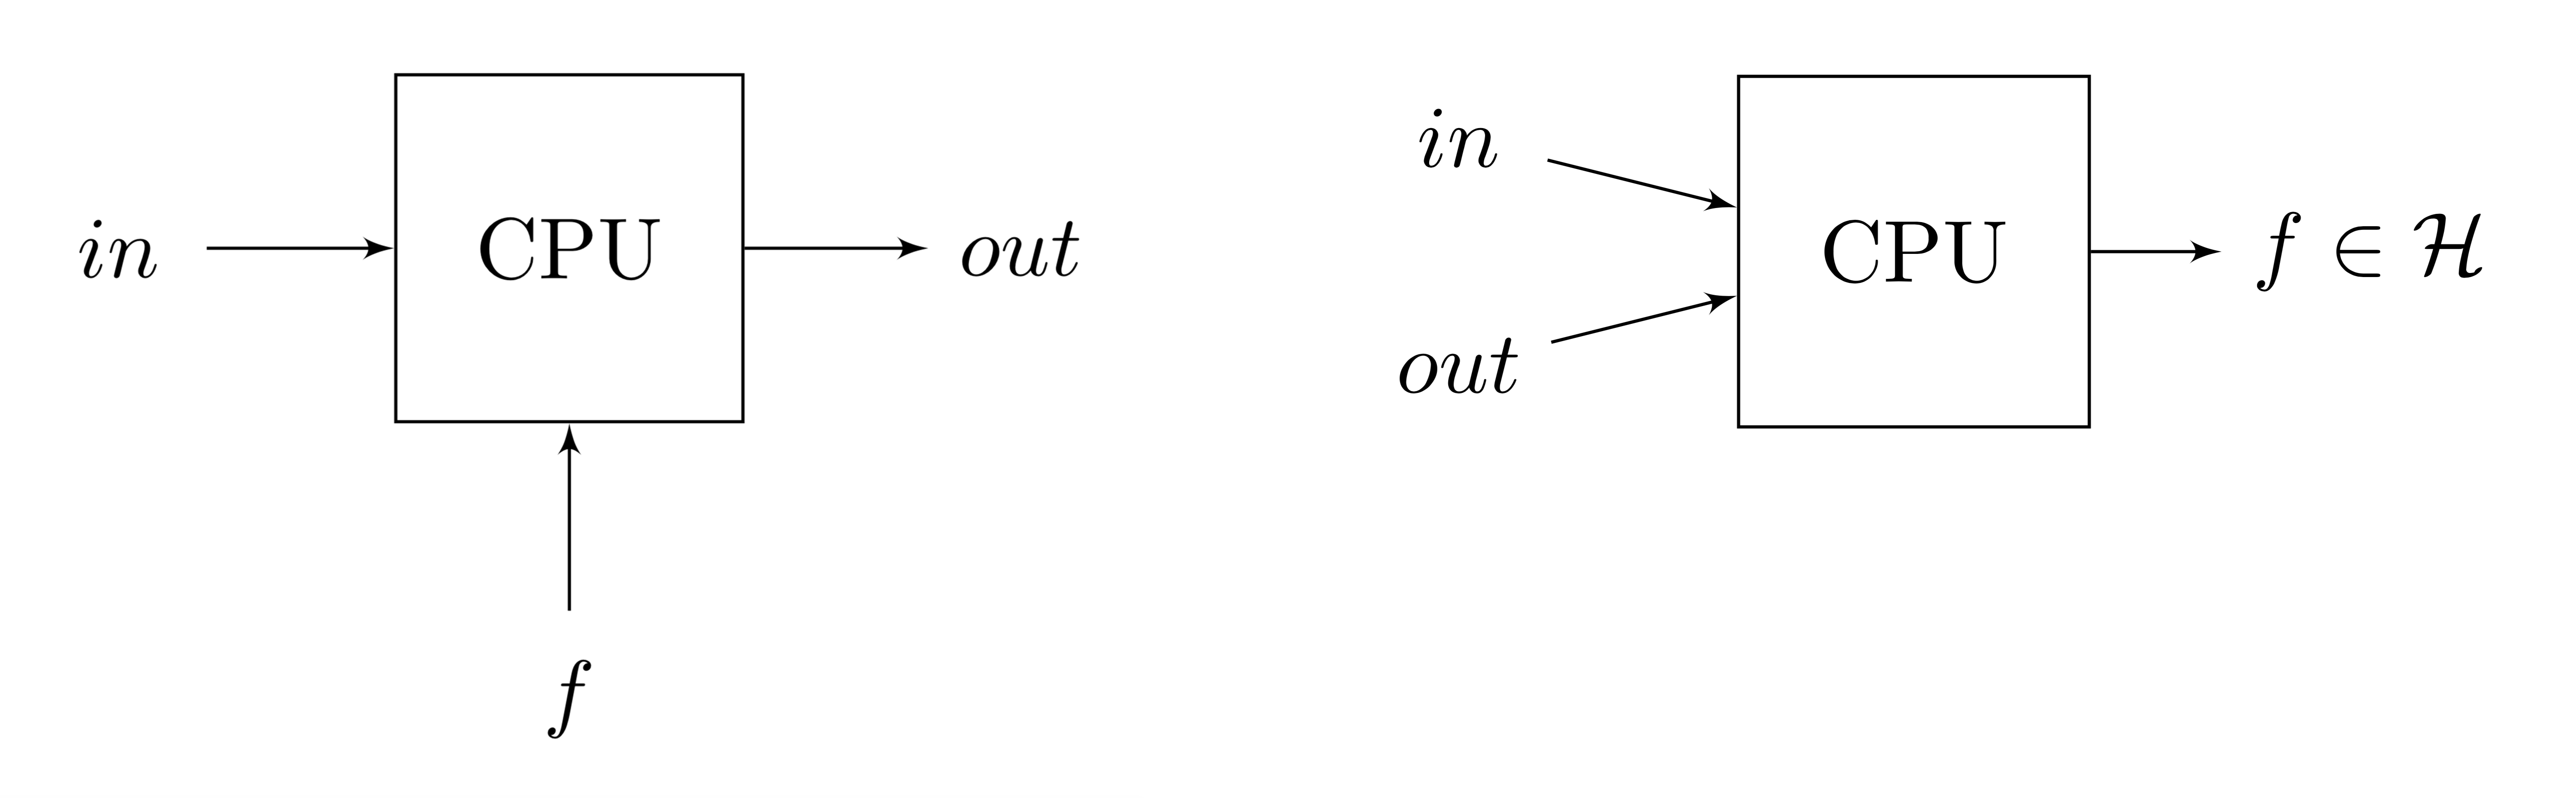
\includegraphics[width=14cm]{img/ml.png}
    \caption{Conceptual comparison of the classic programming approach compared to the one introduced by Machine Learning. On right is shown the classic programming, on left the Machine Learning approach.}\label{ML_programming}
\end{figure}

Machine Learning enables us to perform tasks that are too difficult to solve with fixed programs written and designed by human beings. From a scientific and philosophical point of view, Machine Learning is interesting because developing our understanding of it entails developing our understanding of the principles that underlie intelligence. In this relatively formal definition of the word "task", the process of learning itself is not the task. Learning is our means of attaining the ability to perform the task. Machine Learning tasks are usually described in terms of how the Machine Learning system should process an example. An example is a collection of features that have been quantitatively measured from an object or event that we want the Machine Learning system to process. We typically represent an example as a vector $x\in \mathbb{R}  ^n$ where each entry $x_i$ of the vector is another feature. For example, the features of an image are usually the values of the pixels in the image \cite{deeplearningbook}.

Many kinds of tasks can be solved with Machine Learning. Some of the most common Machine Learning tasks include classification, regression, denoising, anomaly detection. In particular regression was the task to be solved for this thesis work.

In this type of task, the machine is asked to predict a numerical value given some input. To solve this task, the learning algorithm is asked to output a function $f: \mathbb{R} \to \mathbb{R}^n$. This type of task is similar to classification, except that the format of output is different. An example of a regression task is the prediction of the expected claim amount that an insured person will make (used to set insurance premiums), or the prediction of future prices of securities. These kinds of predictions are also used for algorithmic trading.

\section{Deep Learning and Neural networks}\label{deep}
Neural networks, also called feedforward neural networks, or Multi Layer Perceptrons (MLPs), are the quintessential Deep Learning models. The goal of a neural network is to approximate the function $f^\star$. For example, for a classifier, $y=f^\star (x)$ maps an input $x$ to a category $y$. A neural network defines a mapping $y=f(x,\theta)$ and learns the value of the parameters $\theta$ that result in the best function approximation. These models are called feed forward because information flows through the function being evaluated from $x$, through the intermediate computations used to define $f$, and finally to the output $y$. There are no feedback connections in which outputs of the model are fed back into itself. When feedforward neural networks are extended to include feedback connections, they are called  recurrent neural networks which we will discuss in \ref{RNN}.

Feedforward neural networks are called networks because they are typically represented by composing together many different functions. The model is associated with a directed acyclic graph describing how the functions are composed together. 

\begin{figure}
	\centering
	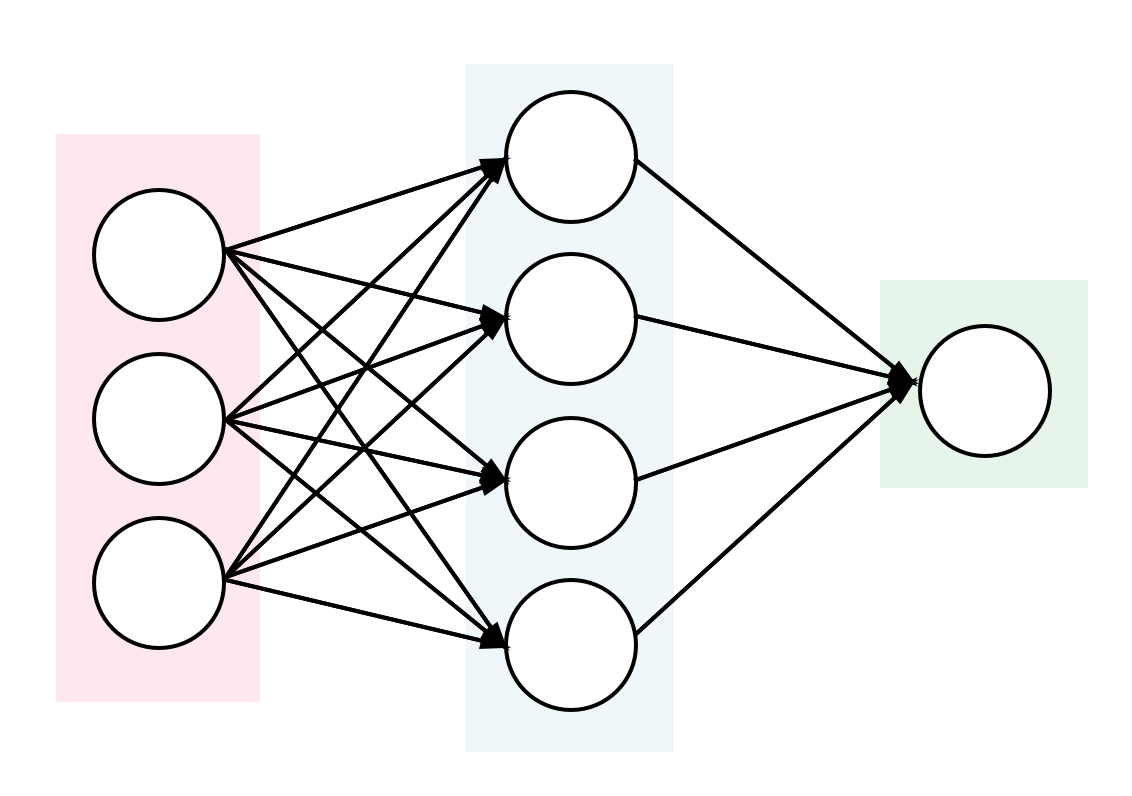
\includegraphics[width=8cm]{img/Single_Hidden_Network.png}
	\caption{The architecture of a single hidden layer network is composed of (from the left) the input layer that receives the data, the hidden layer, and finally the output layer.}
	\label{neuralnetwork}
\end{figure}

With a Single Hidden Layer Neural Network, in Figure \ref{neuralnetwork}, it is possible to approximate any function  $f: \mathbb{R}^n \to \mathbb{R}$, provided that there are enough hidden units (neurons in the intermediate layer between the input and output) \cite{cybenko1989approximation}.
The hidden layer name comes from the fact that the training data does not show the desired output for each of these layers. Adding additional hidden layers to the neural network we begin to talk about a deep network.

\subsection{Recurrent Neural Networks (RNNs)}\label{RNN}
In the previous section we considered feedforward neural networks whose connections did not form cycles. If we relax this condition, and allow cyclical connections as well, we obtain recurrent neural networks, Figure \ref{RNN_fig}, (RNNs). As with feedforward networks, many varieties of RNN have been proposed, such as Elman networks \cite{elman1990finding}, Jordan networks \cite{pollack1990recursive}, time delay neural networks \cite{lang1990time} and echo state networks \cite{jaeger2001echo}.

RNNs, are a family of neural networks for processing sequential data and sequences of values like $x^{(1)}, . . . , x^{(k)}$.
While the difference between a multilayer perceptron and an RNN may seem trivial, the implications for sequence learning are far-reaching. An MLP can only map from input to output vectors, whereas an RNN can, in principle, map from the entire history of previous inputs to each output. Indeed, the equivalent result to the universal approximation theory for MLPs is that an RNN with a sufficient number of hidden units can approximate any measurable sequence to sequence mapping to arbitrary accuracy \cite{hammer2000approximation}. The key point is that the recurrent connections allow a "memory" of previous inputs to persist in the network’s internal state, and thereby influence the network output\cite{graves2012supervised}.

\begin{figure}
	\centering
	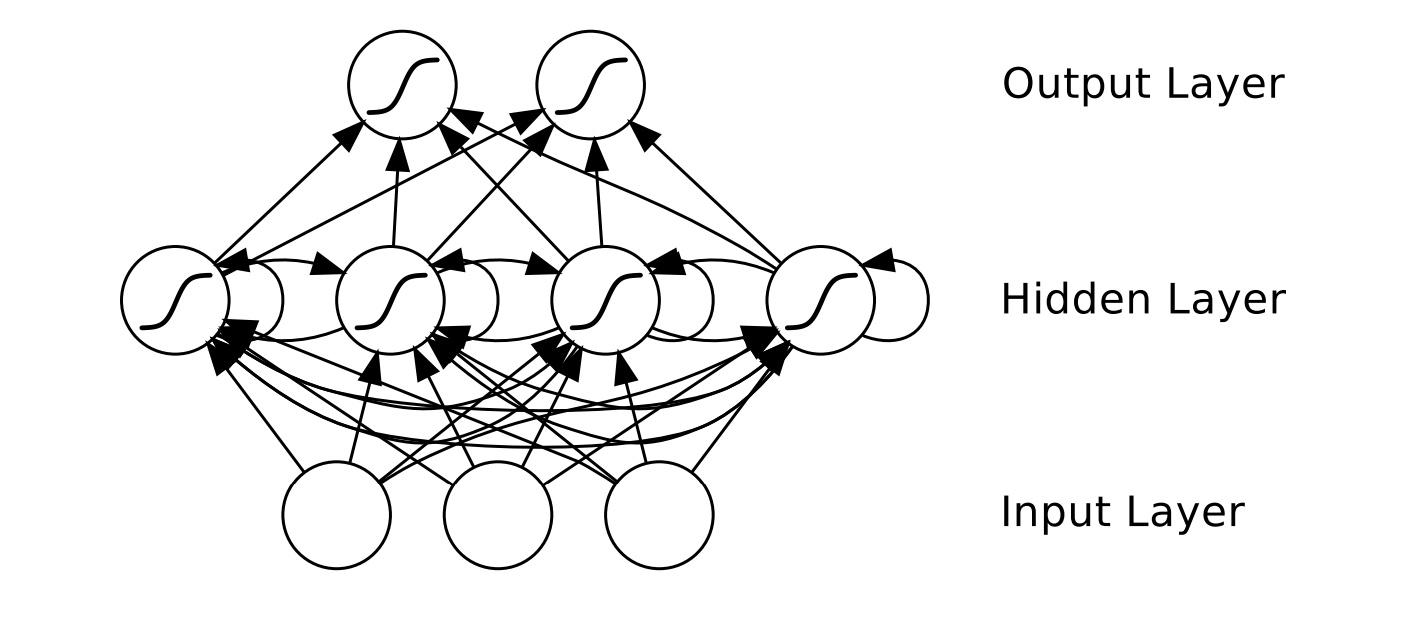
\includegraphics[width=11cm]{img/RNN.png}
	\caption{A recurrent neural network. The figure shown the recurrent connections whose forms cycles, relaxing the condition of feedforward networks.}
	\label{RNN_fig}
\end{figure}

\subsection{Long Short-Term Memory (LSTM)}\label{LSTM_subs}
The LSTM \cite{hochreiter1997long} architecture consists of a set of recurrently connected subnets, known as memory blocks. These blocks can be thought of as a differentiable version of the memory chips in a digital computer. Each block contains one or more self-connected memory cell and three multiplicative units: the input, output and forget gates, that provide continuous analogues of write, read and reset operations for the cells.

\begin{figure}
	\centering
	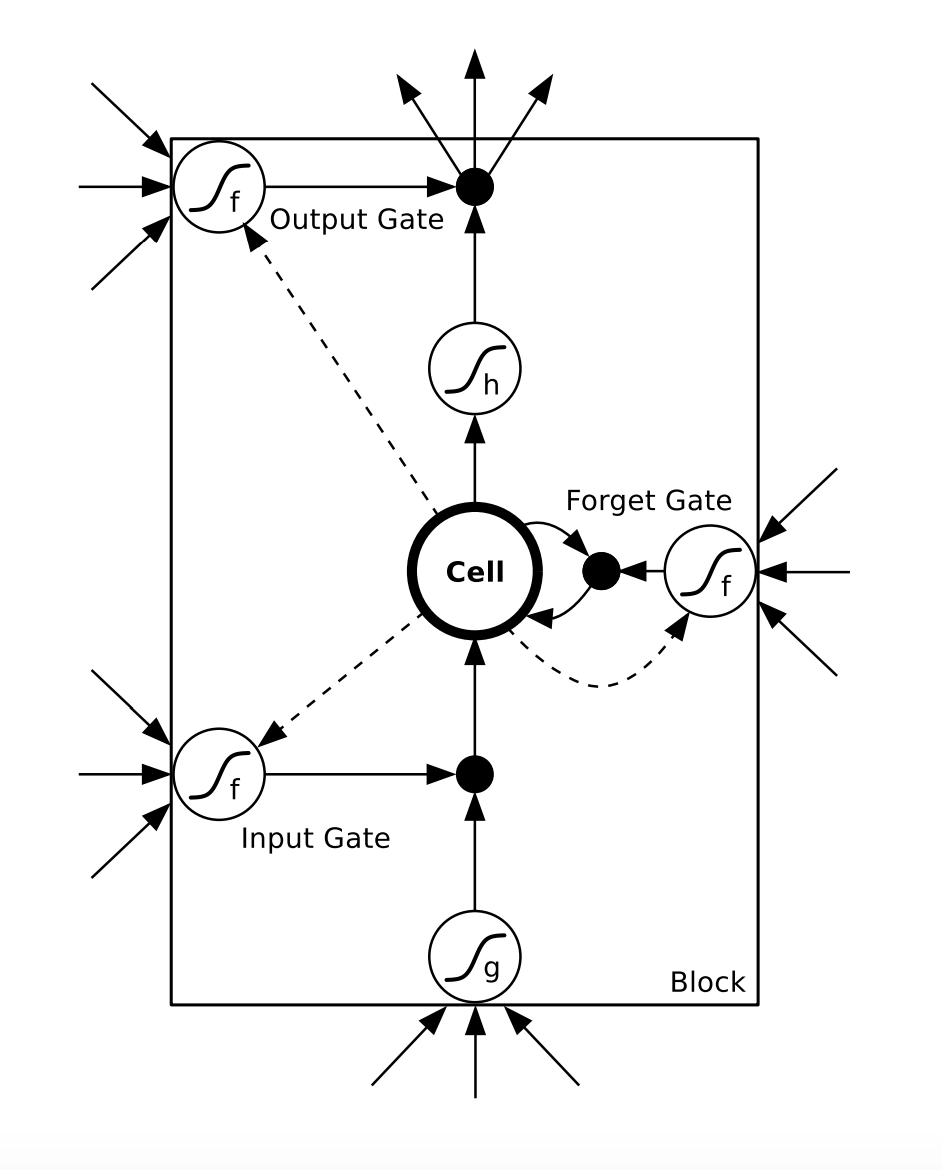
\includegraphics[width=6cm]{img/LSTM_block.png}
	\caption{LSTM memory block with one cell. The three gates are nonlinear summation units that collect activations from inside and outside the block, and control the activation of the cell via multiplications (small black circles). The input and output gates multiply the input and output of the cell while the forget gate multiplies the cell’s previous state. No activation function is applied within the cell. The gate activation function ‘f’ is usually the logistic sigmoid, so that the gate activations are between 0 (gate closed) and 1 (gate open). The cell input and output activation functions (‘g’ and ‘h’) are usually tanh or logistic sigmoid, though in some cases ‘h’ is the identity function.}
	\label{LSTM_block}
\end{figure}

Figure \ref{LSTM_block} provides an illustration of an LSTM memory block with a single cell.
The three gates are nonlinear summation units that collect activations from inside and outside the block, and control the activation of the cell via multiplications (small black circles).
The input and output gates multiply the input and output of the cell while the forget gate multiplies the cell’s previous state. No activation function is applied within the cell. The gate activation function $f$ is usually the logistic sigmoid, so that the gate activations are between 0 (gate closed) and 1 (gate open). The cell input and output activation functions ($g$ and $h$) are usually tanh or logistic sigmoid, though in some cases $h$ is the identity function.
An LSTM network is the same as a standard RNN, except that the summation units in the hidden layer are replaced by memory blocks, as illustrated in Figure \ref{LSTM}. LSTM blocks can also be mixed with ordinary summation units, although this is typically not necessary. The same output layers can be used for LSTM networks as for standard RNNs \cite{graves2012supervised}.

\begin{figure}
	\centering
	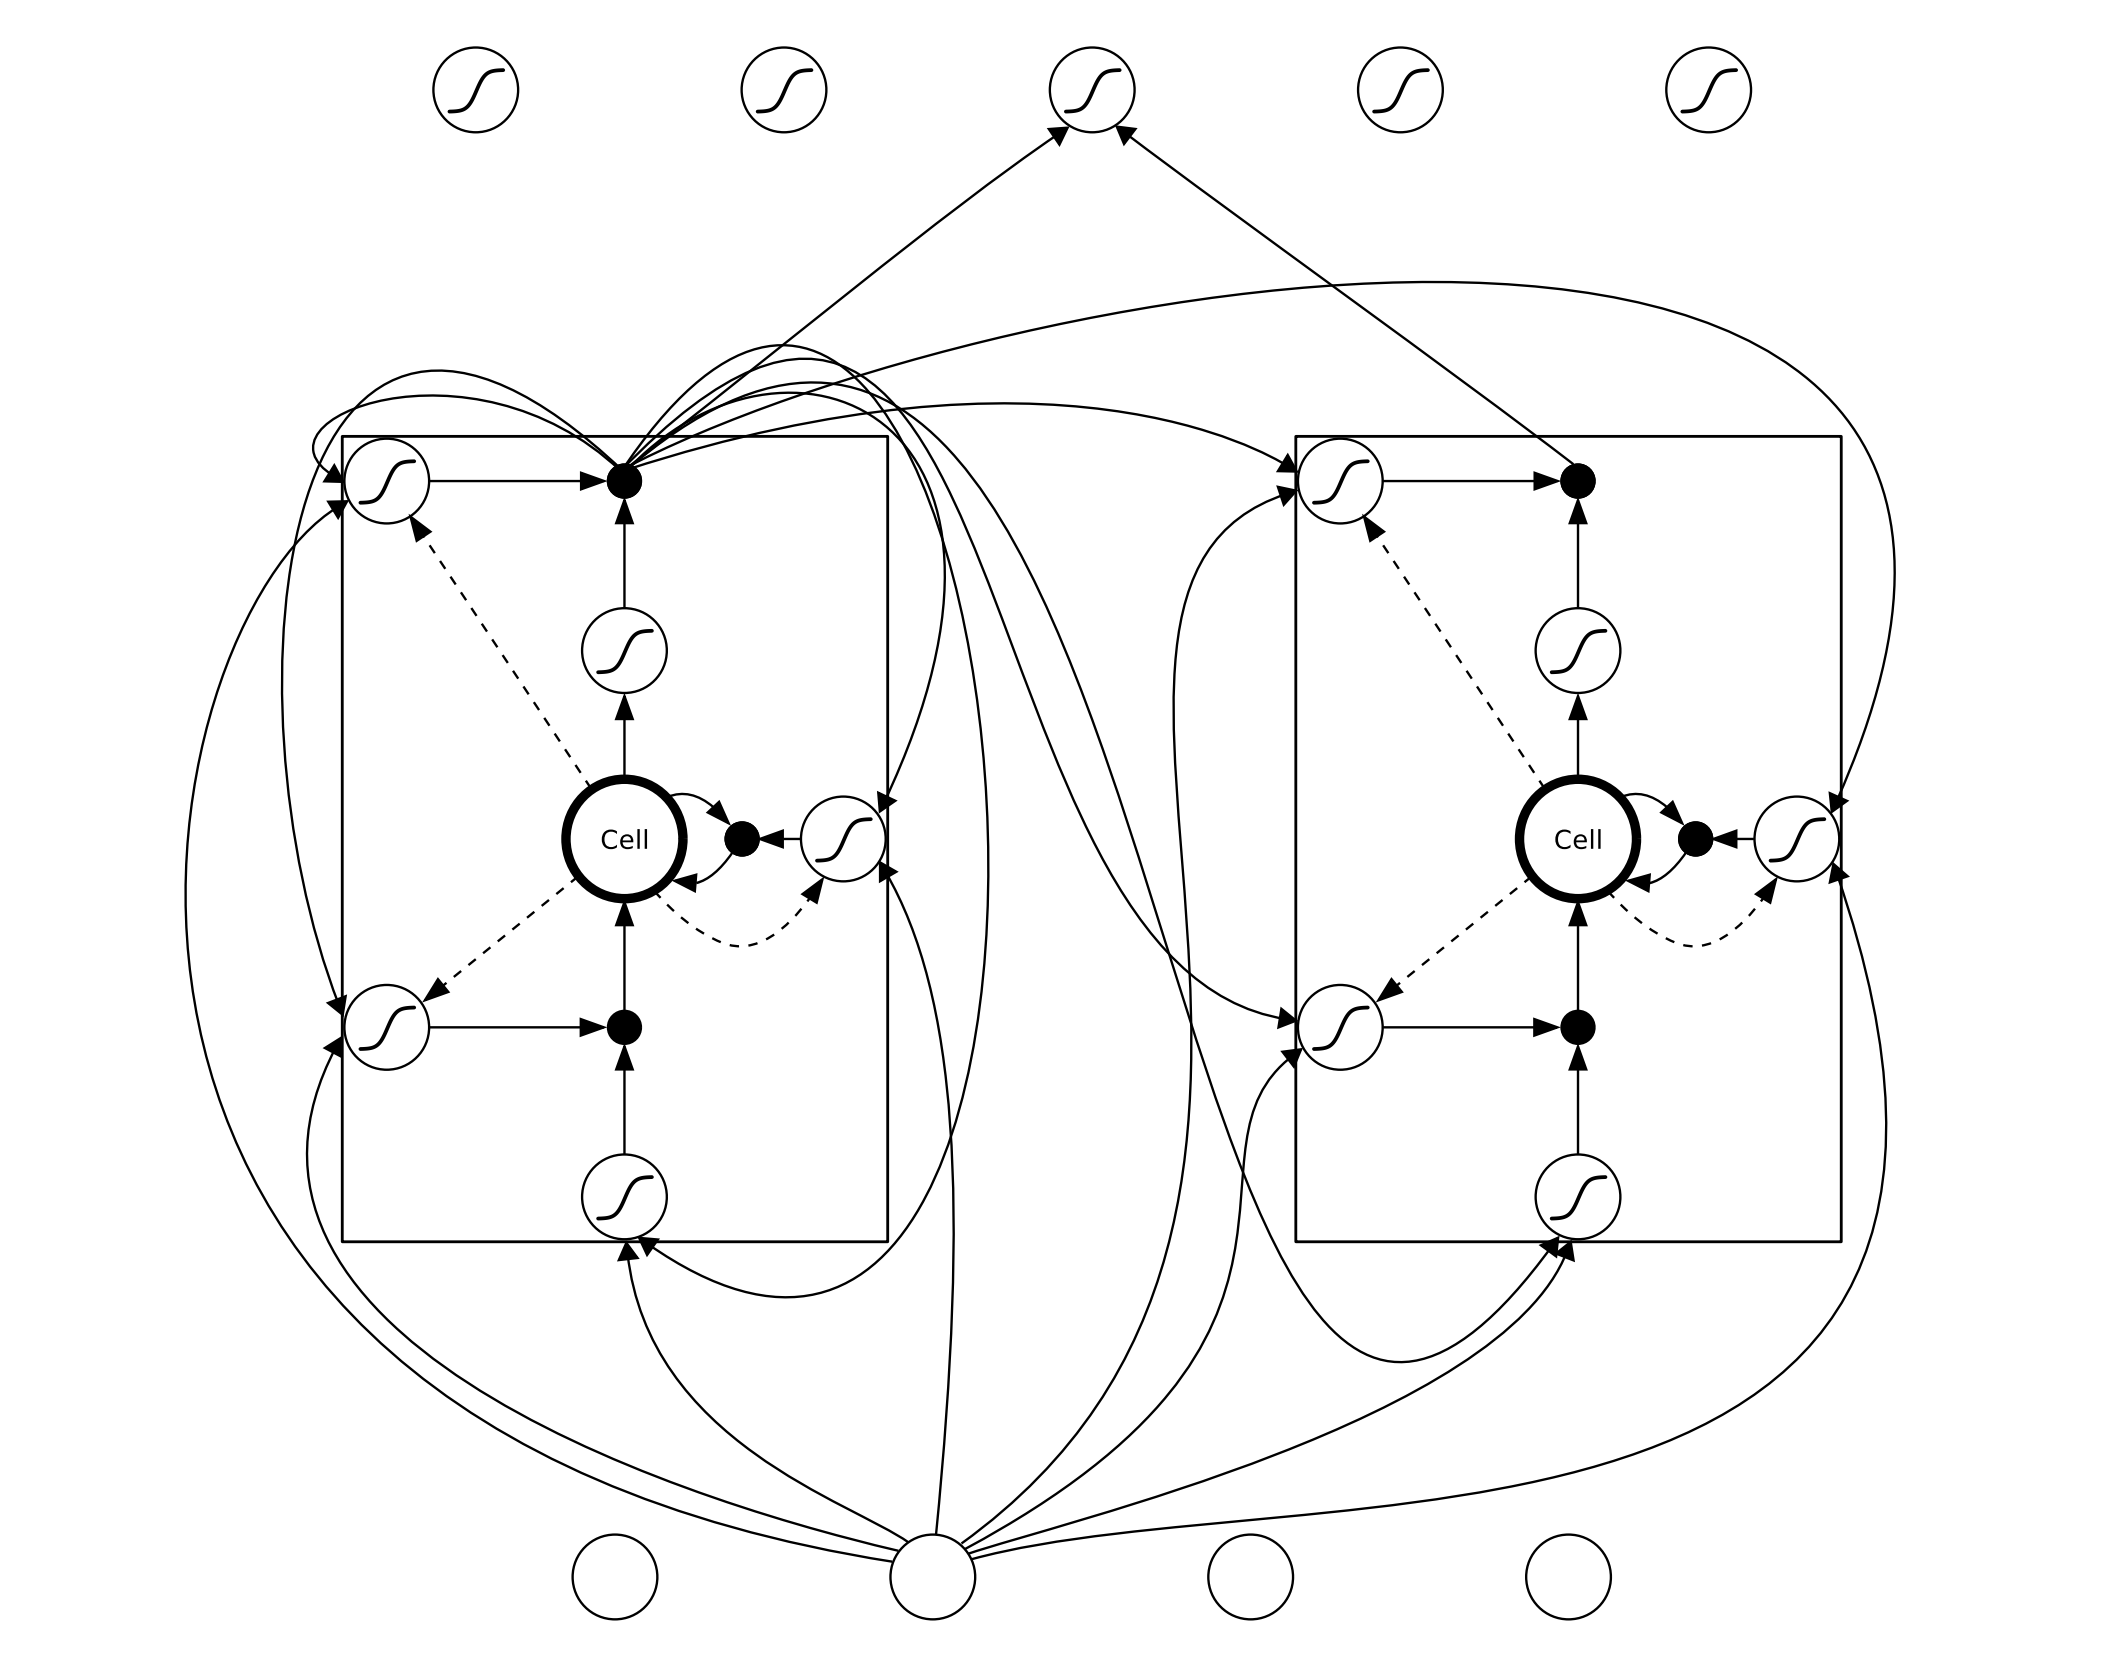
\includegraphics[width=9cm]{img/LSTM.png}
	\caption{An LSTM network.The network consists of four input units, a hidden layer of two single-cell LSTM memory blocks and five output units. Not all connections are shown. Note that each block has four inputs but only one output.}
	\label{LSTM}
\end{figure}

LSTM has been applied to various real-world problems, such
as protein secondary structure prediction \cite{hochreiter2007fast} \cite{chen2005protein}, music generation \cite{eck2002finding}, reinforcement learning \cite{bakker2002reinforcement}, speech recognition \cite{graves2005framewise} \cite{graves2006connectionist} and handwriting recognition \cite{graves2009offline} \cite{graves2008unconstrained}. As would be expected, its advantages are most pronounced for problems requiring the use of long range contextual information.

\subsection{Siamese neural network}
Siamese neural network \cite{bromley1994signature}, Figure \ref{siamese_fig}, consists of two identical sub-networks with shared weights joined at their outputs. This network has two input fields to compare two patterns and one output whose state value corresponds to the similarity between the two patterns.

\begin{figure}
	\centering
	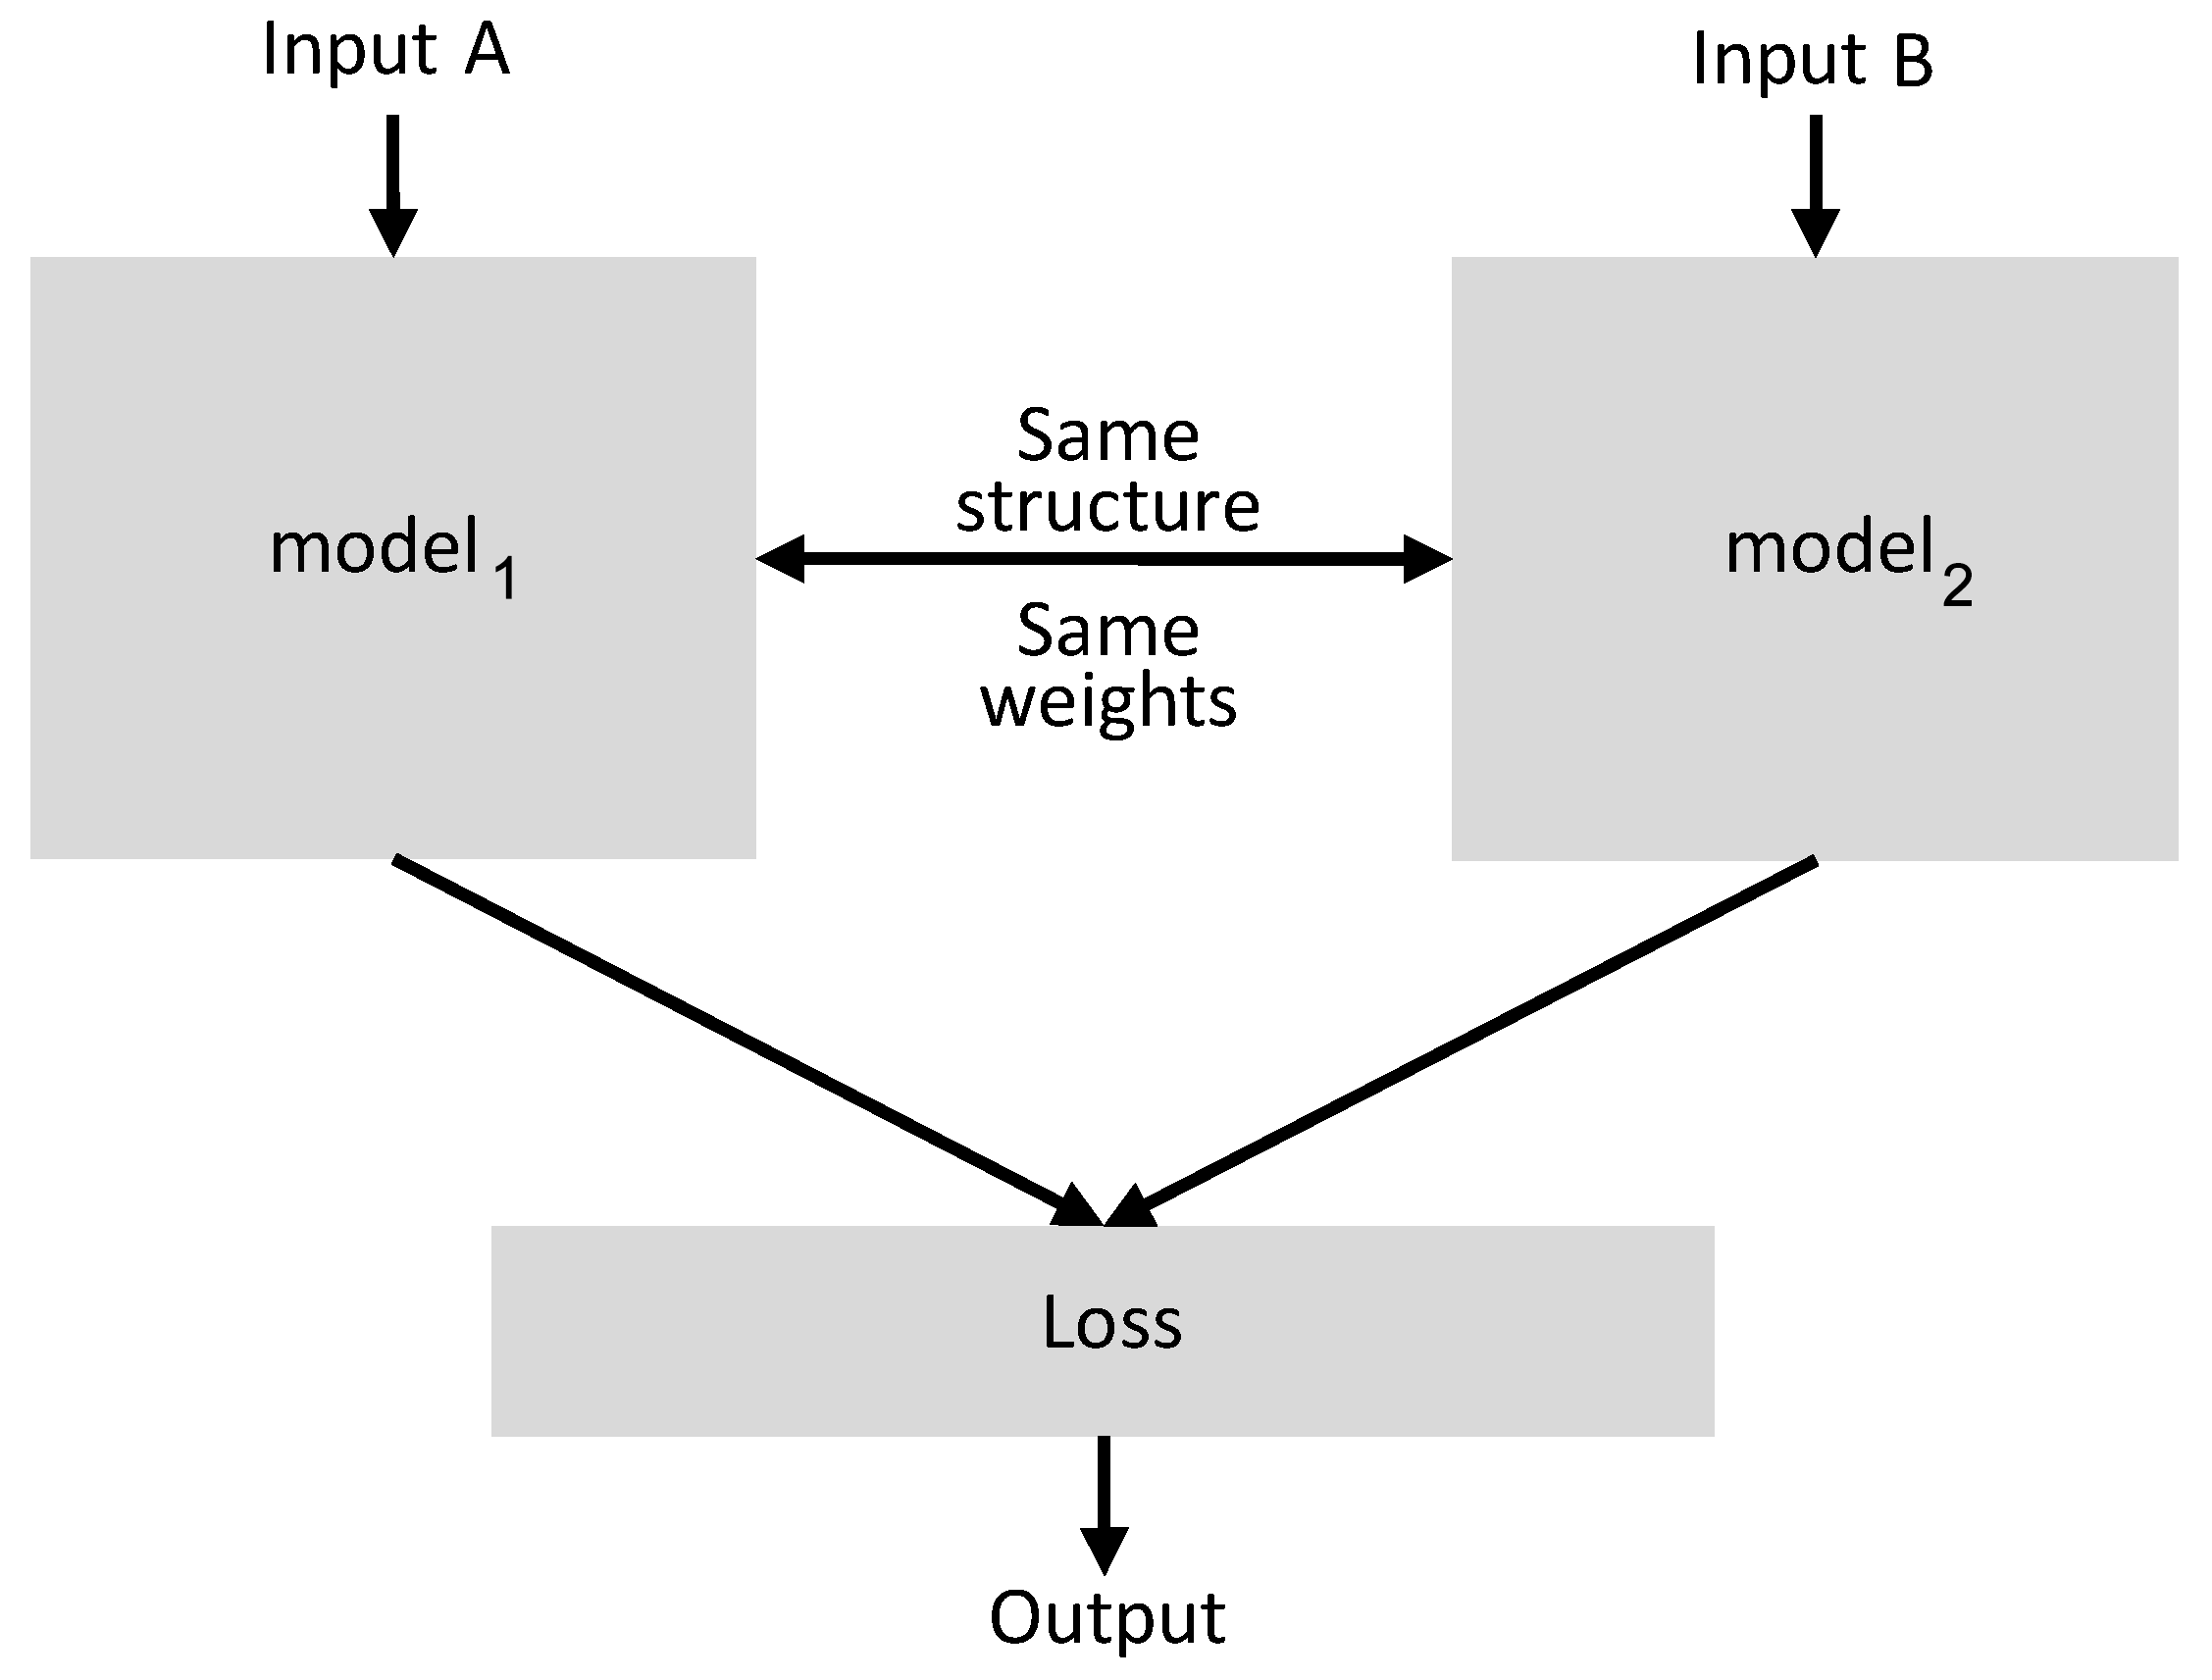
\includegraphics[width=10cm]{img/siamese.png}
	\caption{A generic Siamese neural network. The architecture is composed of the two identical models with shared weights that have different data input. The predictions are then evaluated by a loss function (e.g. Margin ranking loss).}
	\label{siamese_fig}
\end{figure}

The last layer compares the output of the two identical sub-networks and forces the distance, for example, of same category images to be 0 and 1 for the different ones. A contrastive loss function is used for this purpose, which was introduced by Yann LeCun \cite{hadsell2006dimensionality}:

\begin{equation}
L(W, Y, \overrightarrow{X1}, \overrightarrow{X2})=(1-Y)\frac{1}{2}(D_{W})^2 +(Y)\frac{1}{2}\{\max{(0,m-D}_{W})\}^2
\end{equation}

where $Dw$ is the distance output by the network, $Y$ the real value (0/1) and m a parameter which value is determined by the maximum distance chosen (1).
Other loss functions to train the Siamese neural networks are triplet loss \cite{triplet_loss} and Margin ranking loss \cite{rankingloss}. In particular Margin ranking loss was used for the proposed model.

\chapter{BRI\textsubscript{2} Analysis}\label{ch:Ch.3}

This chapter will explain the $BRI_2$ formula and what are the variables involved in the calculation of the risk index. After that the analysis is reported to understand its behavior, the possible limitations and the correlation between the index and the wildlife strike events.
In particular the focus will be on the sensitivity of sightings and $BRI_2$ correlation estimation.

\section{Formula explanation}\label{Formula_explanation}
In order to determine the $BRI_2$, 17 functional groups have been identified, Table \ref{tab-bird_species} , composed of species not strictly taxonomically linked but with common ecological, behavioural and physical characteristics \cite{ENACcircolareAPT_01B}.
\\
The following factors are calculated for each functional group:

\begin{itemize}
    \item $\overline{W}$: the average weight of the $i^{th}$ functional group since monitoring the activity started.
    \item $Ag$: the group specific aggregation index, average number of flocks sighted at the airport since monitoring the activity started.
    \item $BS$: the number of impacts recorded for the $i^{th}$ functional group.
    \item $TFN$: the mean value of flights per year.
    \item $\overline{TFN}$: the mean value of flights per month.
    \item $EOF^{95}$: the 95th percentile of the EOF (Effect On Flight, Table \ref{tab-EOF}).
    \item $DB$: the mean daily number of birds of the $i^{th}$ functional group.
    \item $DF$: the mean daily flight traffic calculated on a monthly basis.
\end{itemize}
After calculating these factors it is possible to determine the value of $BRI_2$ using the following 3 equations:

\begin{equation} \label{eq:3.1}
GF_i=\overline{W_i}\cdot Ag_i \cdot\frac{BS_i}{TFN} \cdot EOF_i ^{95} 
\end{equation}

\begin{equation} \label{eq:3.2}
GSR_i=\frac{GF_i}{\sum_{i=1}^{N}GF_i}\cdot DB_i
\end{equation}

\begin{equation} \label{eq:3.3}
BRI_2=\left(\frac{\sum_{i=1}^{N}GSR_i \cdot DF}{\overline{TFN}}\right)
\end{equation}
where $GF_i$ represents the Group Factor and $GSR_i$ the Group Specific Risk. In equations \ref{eq:3.1}, \ref{eq:3.2}, \ref{eq:3.3}, $i$ indicates a species group (Table \ref{tab-bird_species}) and N is the total number of groups.
In order to understand the behaviour of $BRI_2$, an analysis of these parameters was required.

\section{Parameters analysis}\label{parameters_analysis}
Before proceeding with the analysis of the parameters, a precondition is necessary. After researching Italian airports, the airport chosen to show this analysis was Pisa as it is among the best airports for the quality of the data collected.

The first parameter analyzed was $\overline{W}$, which identifies the average weight of the $i^{th}$ group, independently of the number of sightings.
It is possible to observe from the graph in Figure \ref{W_fig} that this parameter is a constant for each species group, so it makes a constant contribution to the calculation of the Group Factor $GF_i$, eq. \ref{eq:3.1}.

\begin{figure}
	\centering
	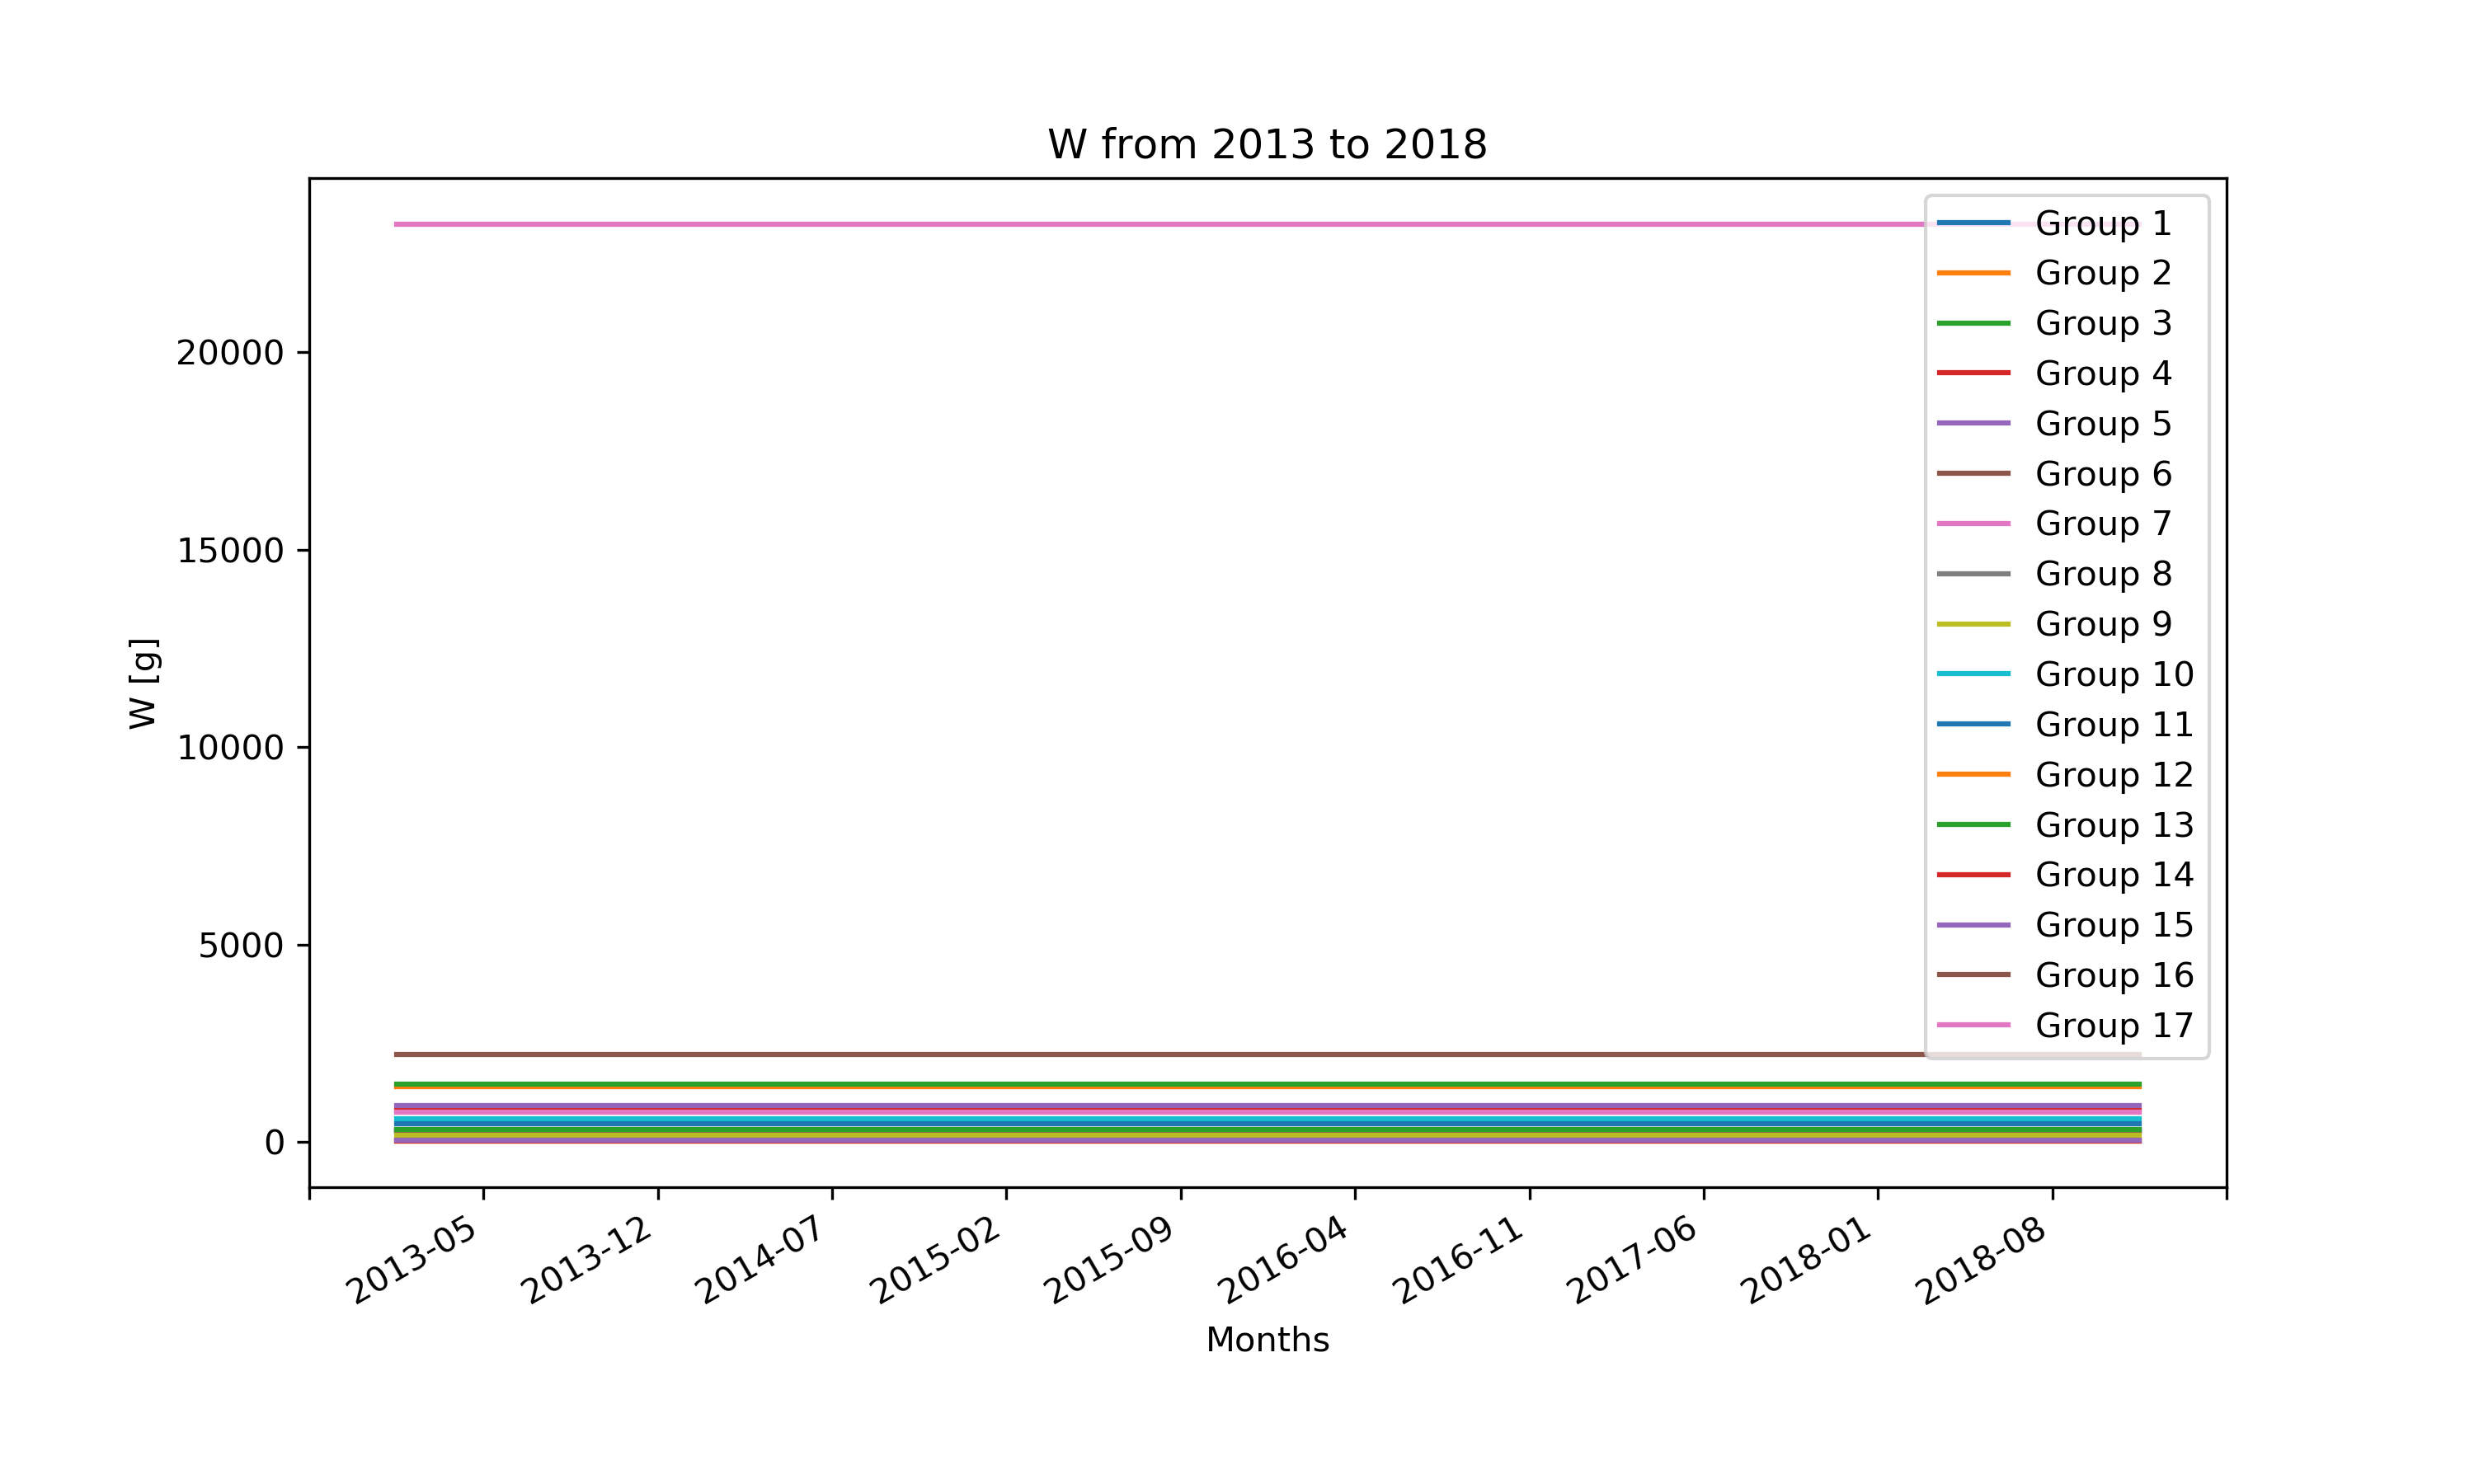
\includegraphics[width=13cm]{img/W.png}
	\caption{$\overline{W}$ parameter from 2013 to 2018 for Pisa airport. The figure shows how over the years analyzed, the weight has remained constant.}
	\label{W_fig}
\end{figure}

The next parameter analysed was $BS$ that is the number of impacts recorded for the $i^{th}$ functional group. This parameter plays an important role in the calculation of the Group Factor. It can only increase (either unchanged) its value as the months increase, as it is not averaged on the calculation period. In the Figure \ref{BS_fig} it is possible see how the BS value is only increased (either unchanged) for each functional group from the beginning of the calculation, 2013, until 2019 excluded.

\begin{figure}
	\centering
	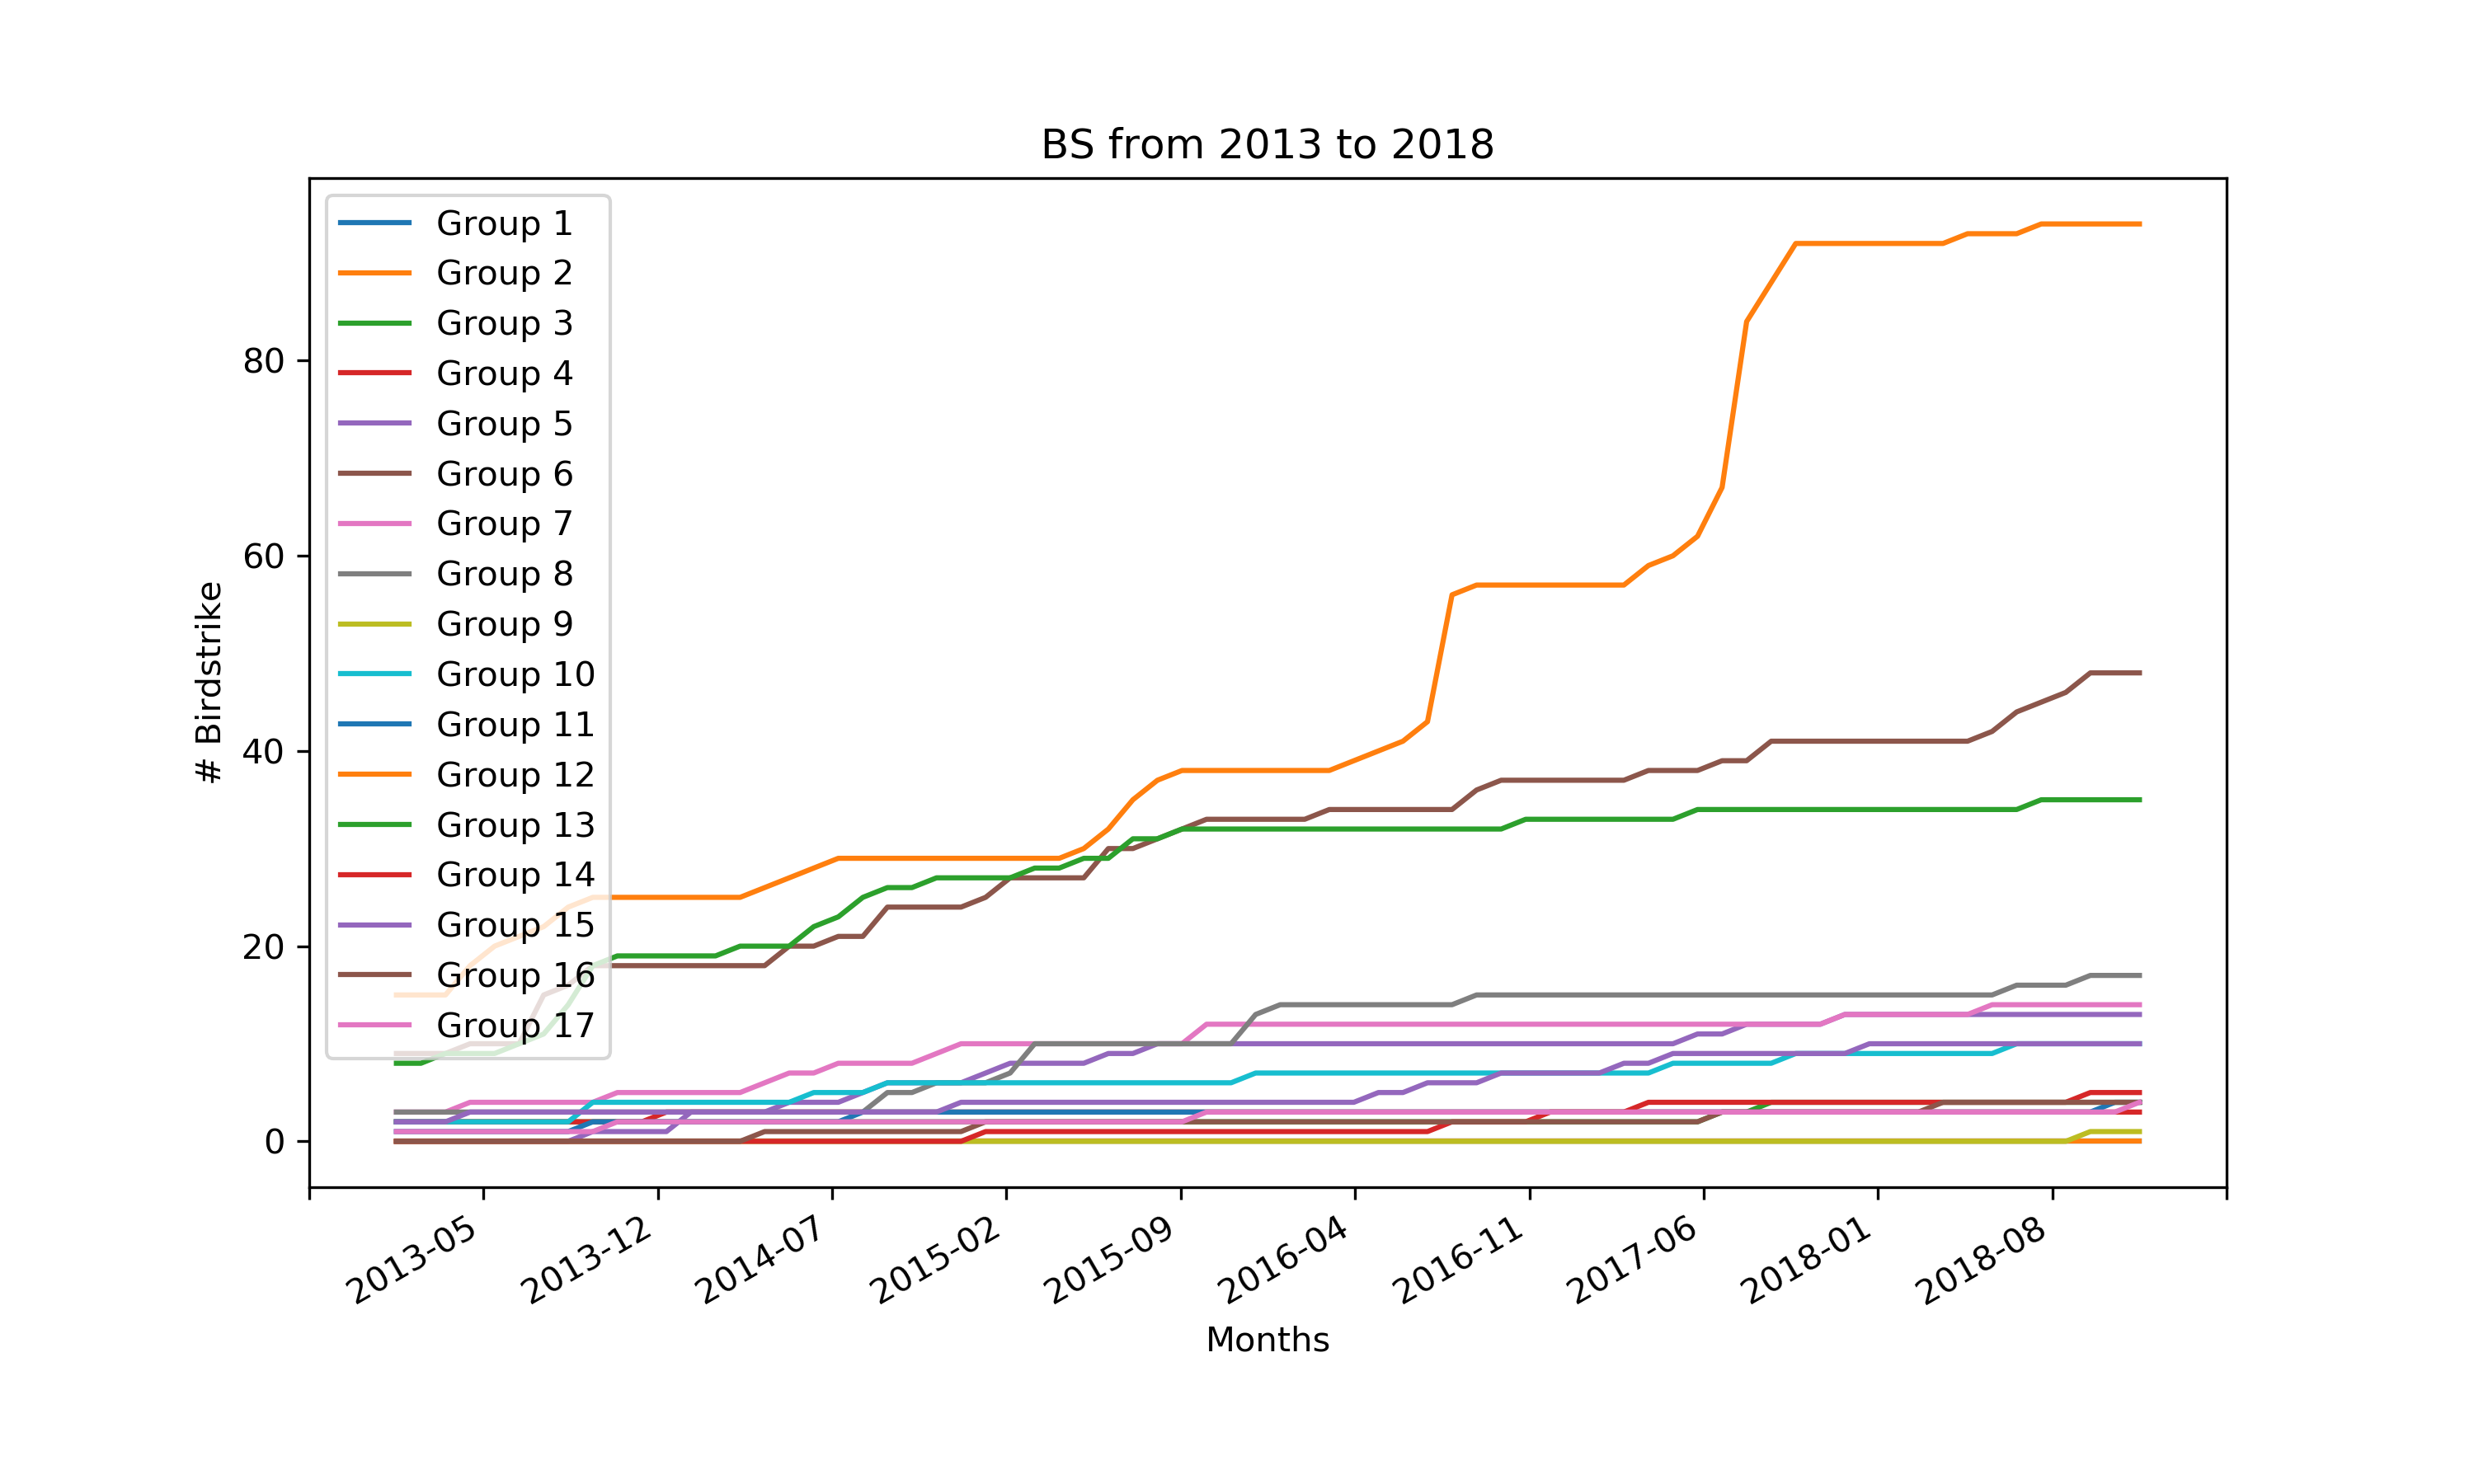
\includegraphics[width=13cm]{img/BS.png}
	\caption{$BS$ parameter from 2013 to 2018 for Pisa airport. The figure shows how, over the years analyzed, the unaveraged $BS$ parameter contributes to a ranking among the species groups.}
	\label{BS_fig}
\end{figure}

The $BS$ parameter is closely related to $EOF^{95}$. This parameter identifies the severity of the birdstrike events for each group and is calculated monthly as the 95th percentile of the $EOF$ values, Table \ref{tab-EOF}. This means that $EOF^{95}$ increases the value of $BS$ and the group factor according to the severity of the birdstrike events, or leaves them unchanged as its minimum value is 1. In Figure \ref{EOF_fig} the $EOF^{95}$ value for each functional group is reported.

\begin{figure}
	\centering
	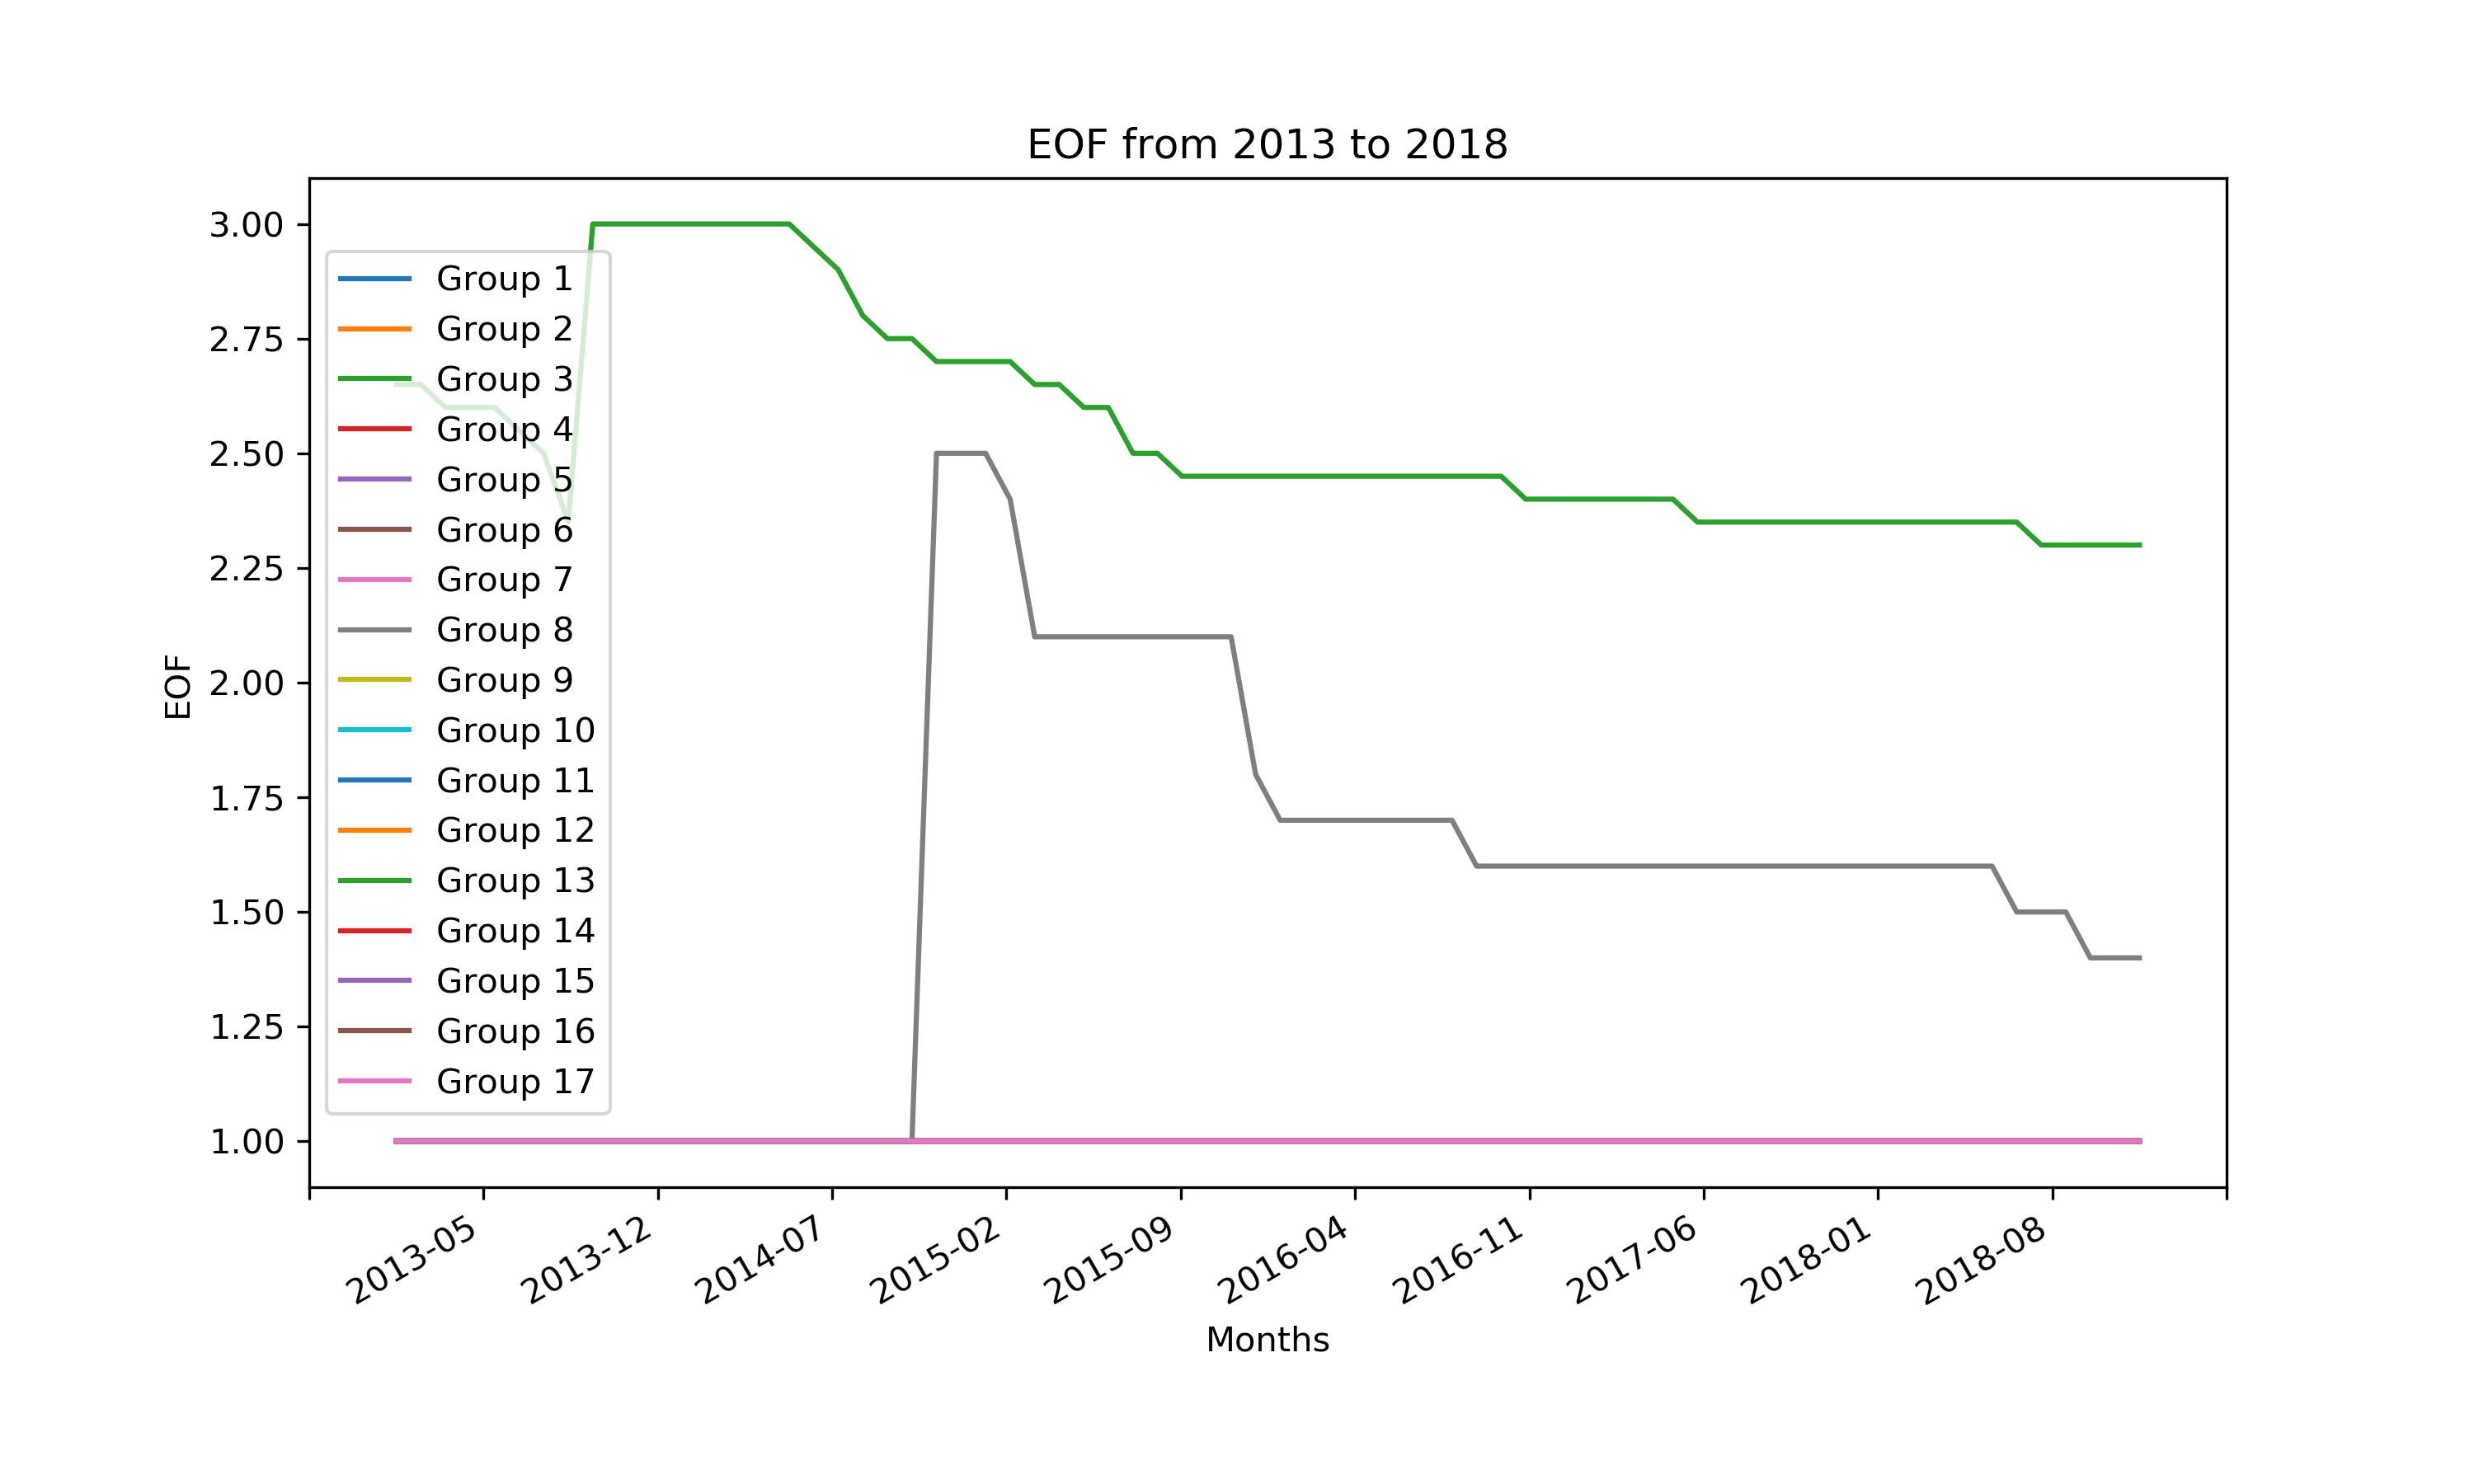
\includegraphics[width=13cm]{img/EOF.png}
	\caption{$EOF^{95}$ parameter from 2013 to 2018 for Pisa airport. The figure shows which group of species has detected birdstrike events with effects on flight. In particular, only 2 groups found these types of events from 2013 to 2018.}
	\label{EOF_fig}
\end{figure}

Another interesting analysis was focused on $Ag$. This parameter is based on sightings and is the average number of flocks sighted at the airport since the monitoring activity started.
The goal of this analysis was to understand the sensitivity of $Ag$ and the contribution of sightings over time as it is averaged on the $BRI_2$ calculation time.
The experiment done was to manually enter sightings in selected months. The months 2014-01 and 2017-12 were chosen to emphasize the desired behavior. In particular, 100 sightings per day were entered for all two months.
The result of the experiment can be seen in Figure \ref{AG_fig}, where the addition of sightings in 2017-02 has a smaller contribution than in 2014-01. This is due to the average over the entire calculation time of the $BRI_2$ and makes the $Ag$ parameter less sensitive to sightings.
\begin{figure}
	\centering
	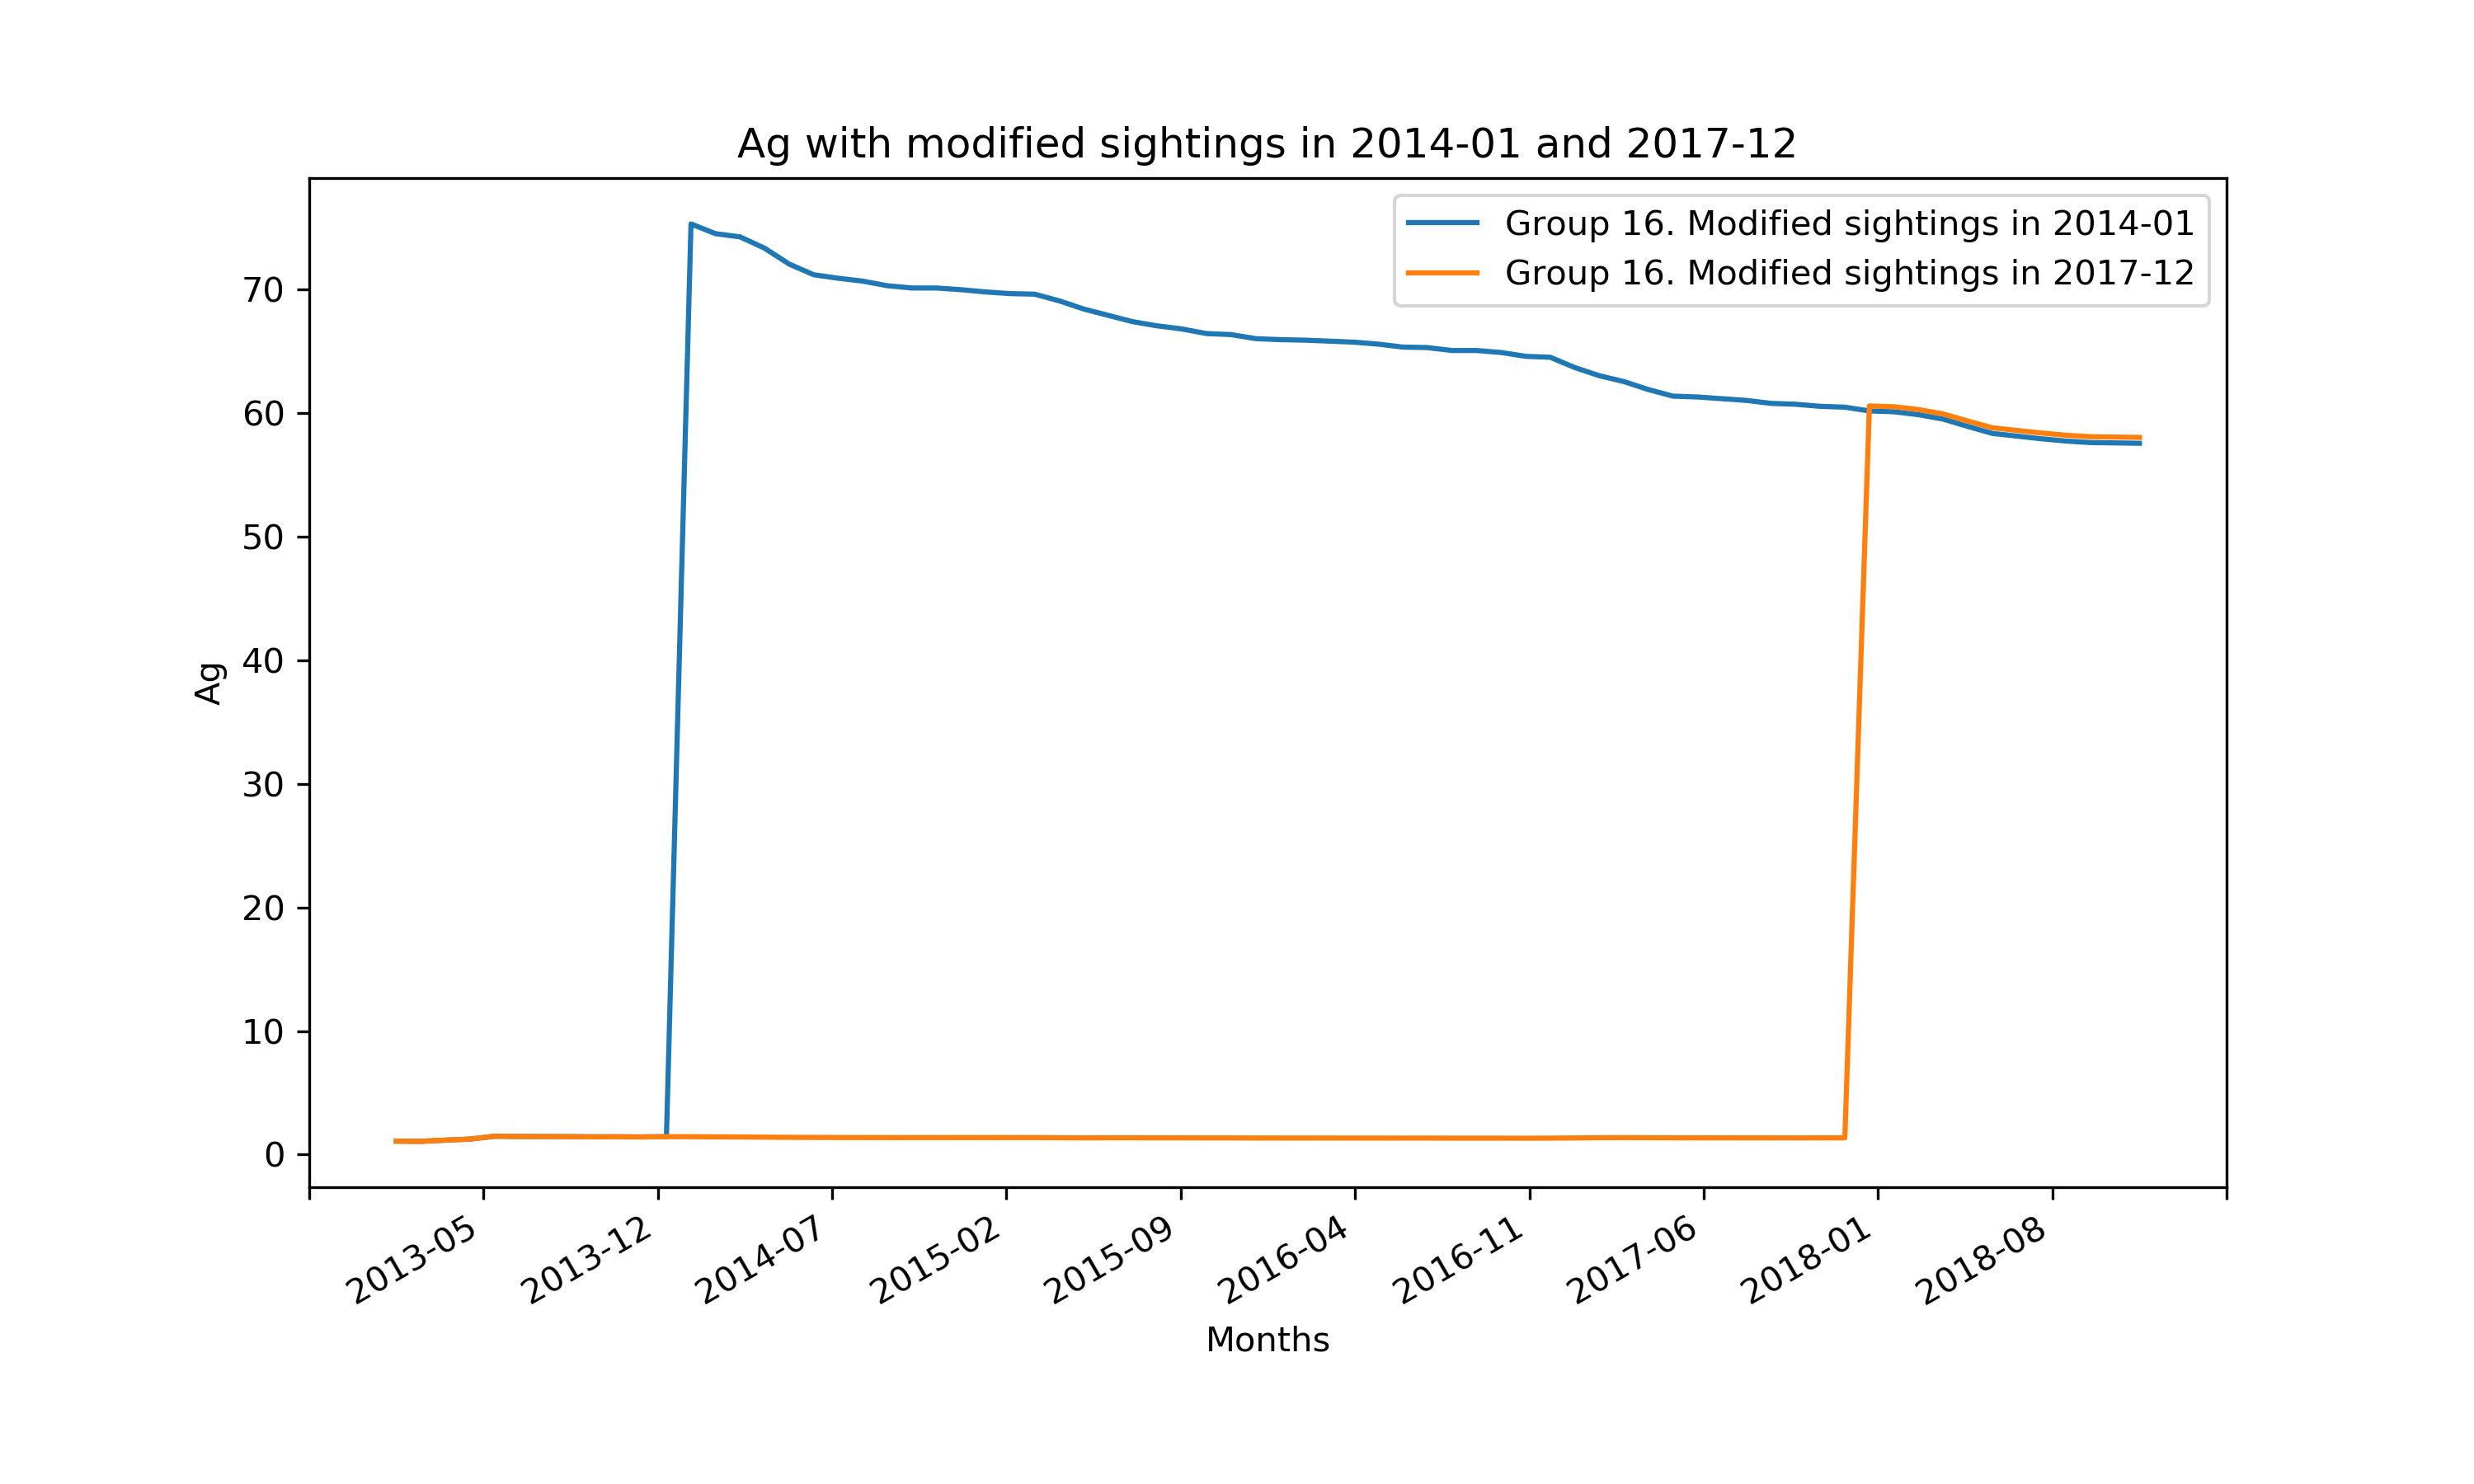
\includegraphics[width=13cm]{img/AG.png}
	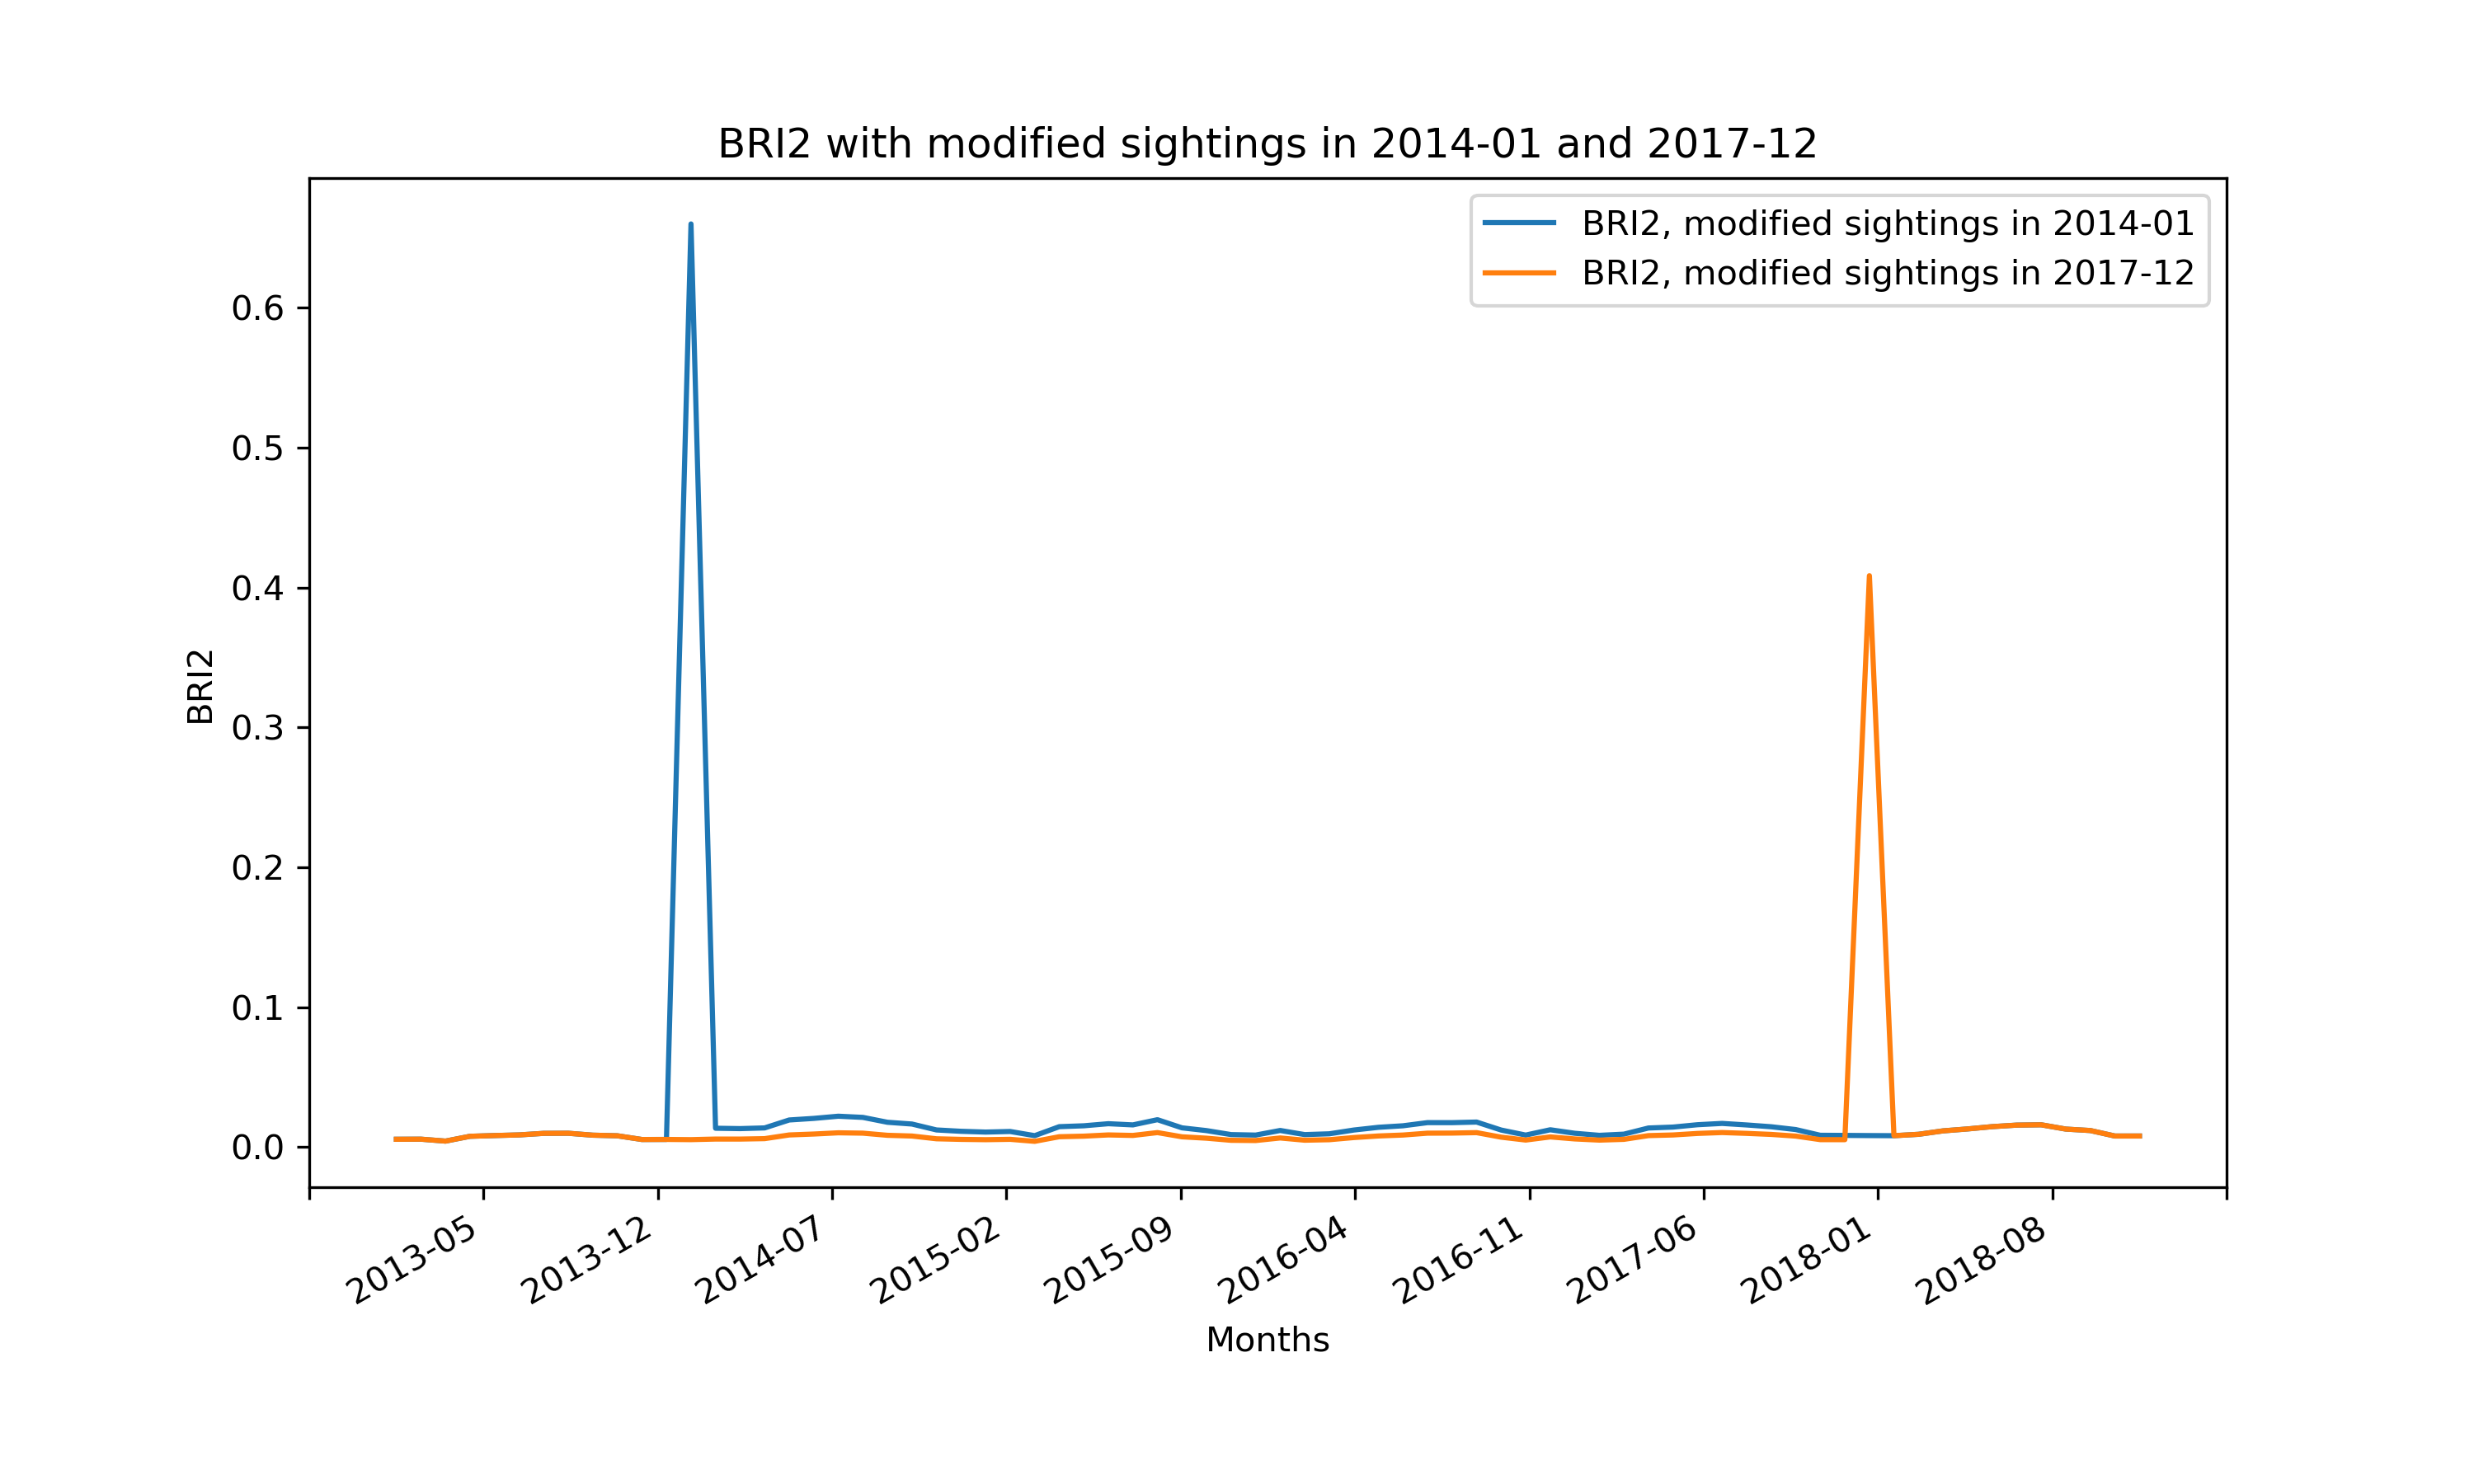
\includegraphics[width=13cm]{img/BRI2_c.png}
	\caption{$Ag$ and $BRI_2$ parameter with modified sightings in 2014-01 and 2017-12. The figure shows (above) the effect of the average on the $Ag$ parameter. This causes the effect of sightings to degrade over time. In particular it has been shown the effect on 1 group out of 17. The figure (below), shows the effect of the average $Ag$ in the $BRI_2$ calculation. This causes a degradation of the effect of sightings over time that is also observed in the $BRI_2$ value.}
	\label{AG_fig}
\end{figure}
This behaviour can also be observed in the calculation of the $BRI_2$ by making the group factor depend exclusively on sightings. The rusult of this experiment is shown in Figure \ref{AG_fig}.
No specific analysis has been made for the remaining parameters. In particular $TFN$ and $\overline{TFN}$ are normalizers for equations \ref{eq:3.2} and \ref{eq:3.3} and $DB$ is a daily average of sightings  not dependent on time.

After these analyses it is clear that the fundamental parameters for the calculation of $BRI_2$ are $BS$, $Ag$, $EOF^{95}$. Some problems have been identified:
\begin{itemize}
    \item $Ag$ loses sensitivity to sightings over time.
    \item  $BS$ is a cumulative parameter that stores birdstrike events from the beginning of the $BRI_2$ calculation and is not averaged.
    \item  $EOF^{95}$ contributes to the group factor increase by boosting the effects of $BS$.
\end{itemize}
The group factor $GF$ can be considered as a sort of reputation among the species groups that over time creates a ranking of danger gradually less related to sightings but closely related to the birdstrike events of the past.
This means that the $BRI_2$ value will be higher if more dangerous groups are sighted independently to the amount of elements sighted.

\section{Correlation with wildlife strike events}\label{smooth}
A second study has been done to understand if $BRI_2$ is a good
tool capable of describing an airport-specific wildlife strike risk.
If $BRI_2$ is a good risk-index it must have a good correlation with the events of wildlife strike.

The first step of this study was to generate a curve that would describe as accurately as possible the evolution of wildlife strike events over time.
To generate the curve a Gaussian filter was chosen and correlation tests were performed with different $\sigma$ values (standard deviation for Gaussian kernel), in particular $\sigma = [0.5, 1.0, 1.5, 2.0]$, and for comparison $BRI_2$ and the curve of wildlife events have been normalized.

The measure of correlation chosen was the correlation of Spearman. It estimates how well the relationship between two variables can be described using a monotonous function. The sign of the Spearman correlation indicates the direction of association between $X$ (the independent variable) and $Y$ (the dependent variable). If $Y$ tends to increase when $X$ increases, the Spearman correlation coefficient is positive. If $Y$ tends to decrease when $X$ increases, the Spearman correlation coefficient is negative. A Spearman correlation of zero indicates that there is no tendency for $Y$ to either increase or decrease when $X$ increases.
Equation \ref{eq_spearman} show the formula for the calculation of the Spearman correlation for a sample of size n. The n raw scores $X_i, Y_i$ are converted to ranks rg($X_i$), rg($Y_i$) and $\mathit{r_s}$ is computed as:

\begin{equation}\label{eq_spearman}
\mathit{r_s} = \frac{\mathrm{cov(\mathrm{rg_\mathcal{X}}, \mathrm{rg_\mathcal{Y}}})}{\sigma_{\mathrm{rg_\mathcal{X}}}\sigma_{\mathrm{rg_\mathcal{Y}}}}
\end{equation}
where:

\begin{itemize}
    \item $\mathrm{cov(\mathrm{rg_\mathcal{X}},\mathrm{rg_\mathcal{Y}}})$ is the covariance of the rank variables.
    \item $\sigma_{\mathrm{rg_\mathcal{X}}}\sigma_{\mathrm{rg_\mathcal{Y}}}$ are the standard deviations of the rank variables.
\end{itemize}
Only if all n ranks are distinct integers, it can be computed using the formula in equation \ref{eq_spearman_2}:

\begin{equation}\label{eq_spearman_2}
\mathit{r_s} = 1 - \frac{\sum_{i} d^2_i}{n-(n^2-1)}
\end{equation}
where $d_i$ = rg($X_i$), rg($Y_i$).

It is possible to observe the result of the study for Pisa airport in Figure \ref{corr_curve} and \ref{corr_scatter}.
\begin{figure}
	\centering
	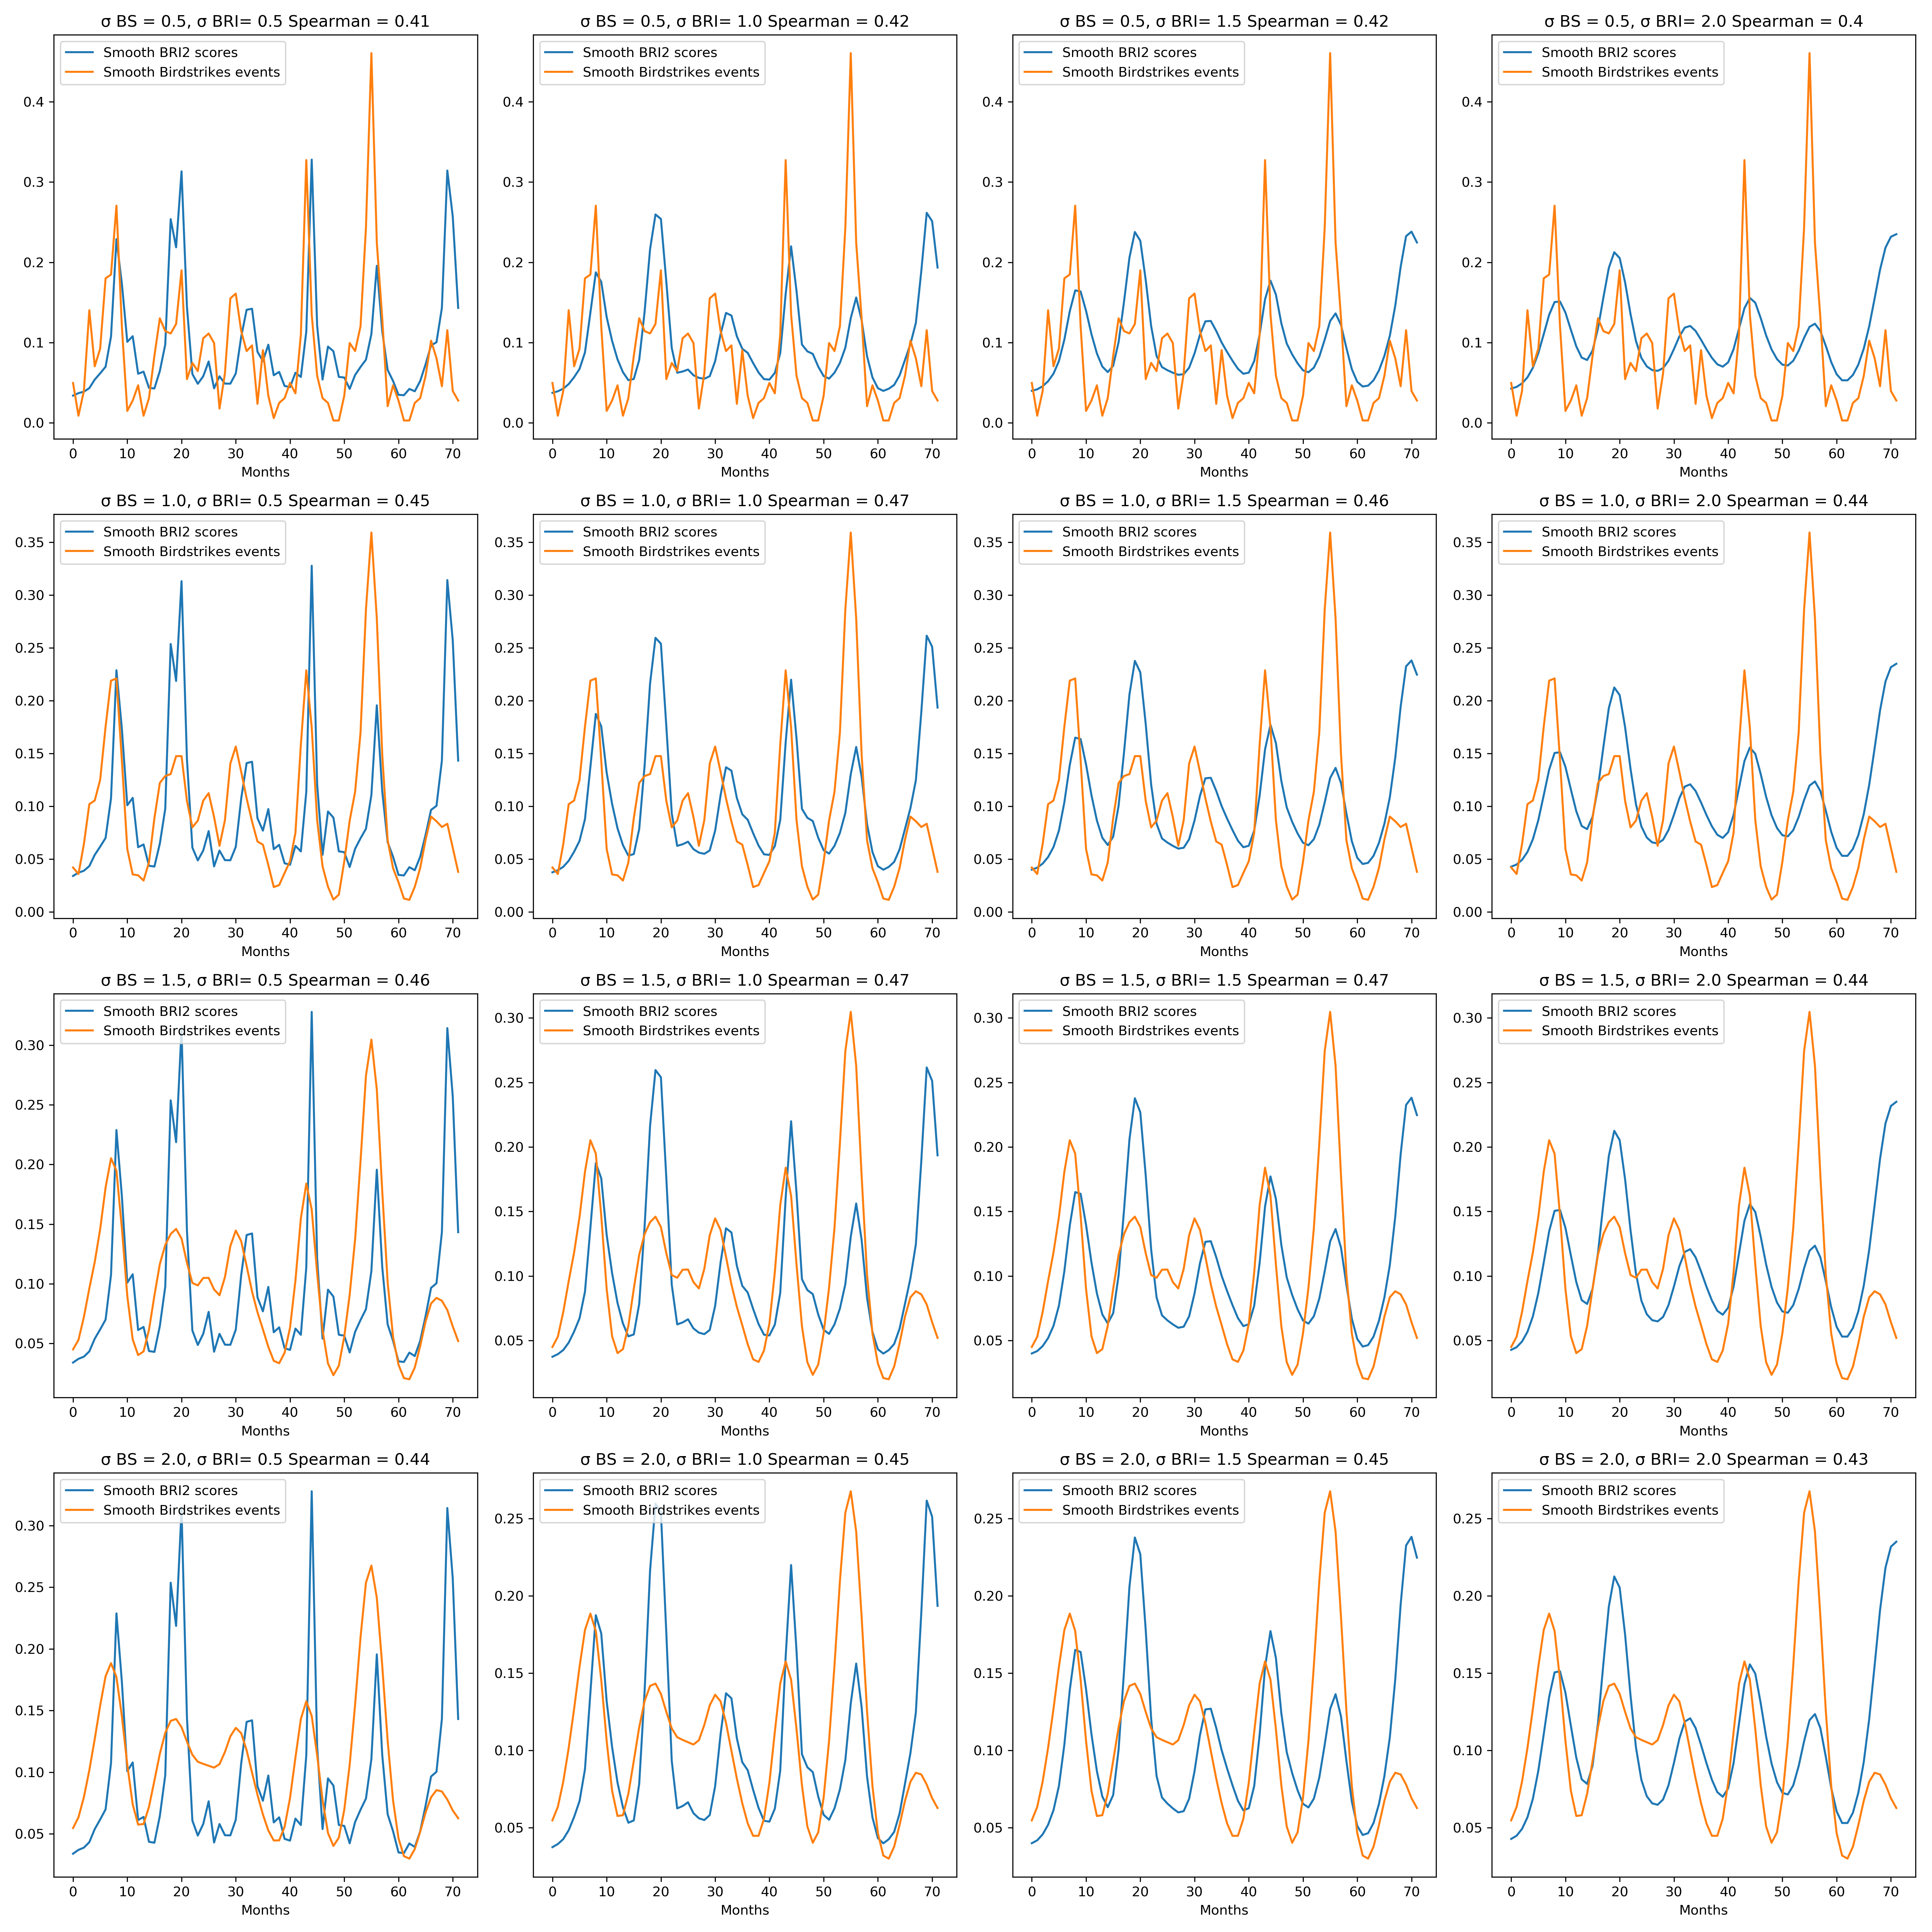
\includegraphics[width=14cm]{img/corr_curve.png}
	\caption{Spearman correlation between $BRI_2$ and the wildlife strike curve. Each subplot shows the correlation between the two variables with a different level of smoothing given by the Gaussian filter.}
	\label{corr_curve}
\end{figure}
\begin{figure}
	\centering
	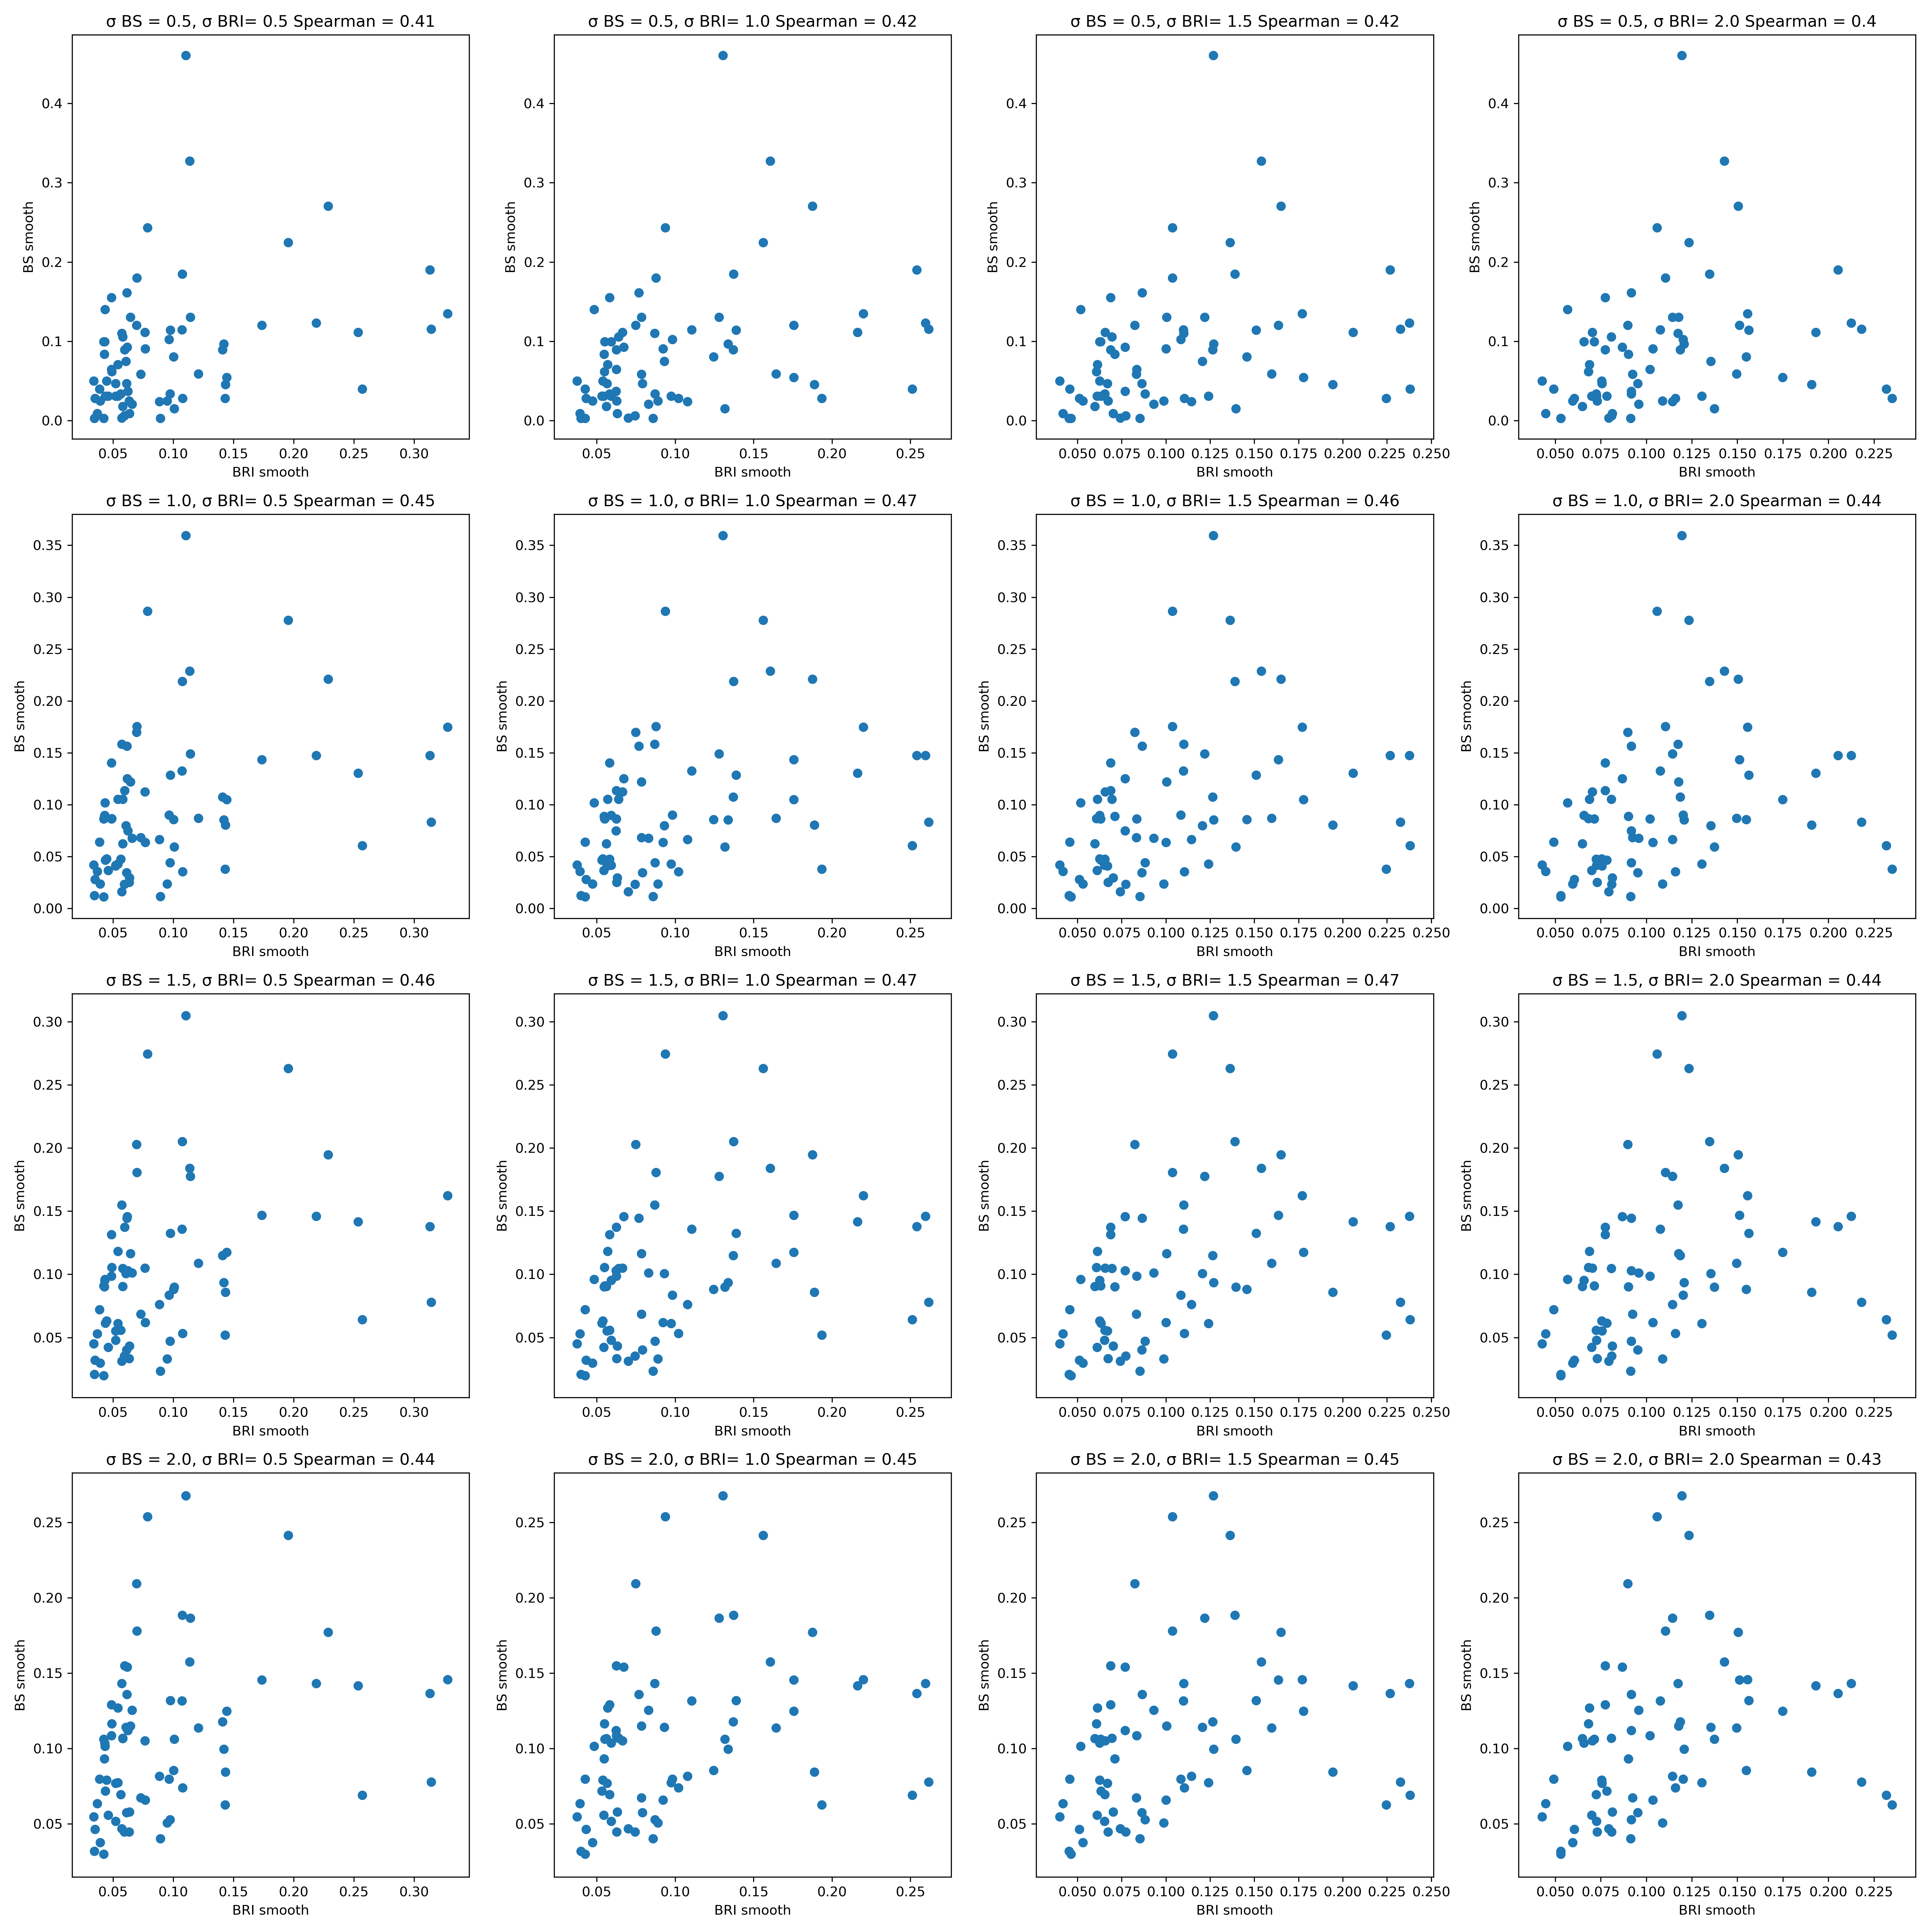
\includegraphics[width=14cm]{img/corr_scatter.png}
	\caption{Spearman correlation between $BRI_2$ and the wildlife strike curve. Each scatter-subplot shows the correlation between the two variables with a different level of smoothing given by the Gaussian filter.}
	\label{corr_scatter}
\end{figure}
Each subplot shows the Spearman correlation between the two variables with a different level of smoothing given by the Gaussian filter.
In particular, in Figure \ref{corr_scatter} scatter plots are used to display $BRI_2$ and wildlife strikes' values in cartesian coordinates.
The results show that for Pisa at most Spearman correlation has value 0.47, obtained in 3 cases out of 16, which means a not so high correlation.

\begin{table}
	\centering
	\scalebox{1}{
	\begin{tabular}{@{}ccc@{}}
		\toprule
		Airport & Spearman correlation \\	\midrule
		Florence & 0.17 \\
		Pisa & 0.47 \\
		Bologna & 0.26\\
		Milan-Malpensa &  -0.14 \\
		Milan-Linate & -0.28 \\
		Verona & 0.6 \\
		Catania & 0.49 \\
	    Brescia & 0.31 \\	\bottomrule
	\end{tabular}}
	\caption{Correlation values between $BRI_2$ and wildlife strikes events of some Italian airports.}
	\label{tab-corr}
\end{table}

The Table \ref{tab-corr} shows the results of the correlation in other Italian airports. Also for other airports the correlation with wildlife events is not so high, where the highest correlation found was 0.5 at Catania airport.

The next chapter deals with the proposed model. The purpose of this model is to provide a new risk-index closer related to $BRI_2$.

\subsection{Discussion}

After the analysis performed and discussed in this chapter, the $BRI_2$ risk index is dependent on variables (described in \ref{Formula_explanation}) which are certainly easy to explain and understand. But this makes the $BRI_2$ an easy to calculate but empirical index.
We have identified in section \ref{parameters_analysis} important problems related to the factors involved:
$Ag$ is a averaged parameter that loses sensitivity over time, $GF$ is a reputation of species groups not very dependent on sightings but related to the number of birdstrike events caused in the past, given the nature of variables $Ag$ and $BS$ which is cumulative over time.
Finally, the $BRI_2$ has proven to be poorly correlated to historical birdstrike events collected on all the airports tested in the analysis (Table \ref{tab-corr}).

\chapter{Proposed Model} \label{ch:Ch.4}
After analyzing the $BRI_2$ in the previous chapter, the proposed model will be presented. In particular, this chapter will describe in detail the model implemented starting from the dataset used and the pre-processing techniques to the chosen architecture. The goal of the model is to provide a daily risk-index based on the observations of the previous days. In particular, given an airport, the model looks at a window of $K$ days and provides the risk-value for the following day. 

\section{Dataset}
The dataset used includes data from more than 100 Italian airports, including military airports and internal divisions dedicated to internal and external naturalistic research. Data quality varies from airport to airport.
The dataset includes all daily data that derives from the Bird Strike Reporting Form, which is divided into Impact Reporting Form and Fauna Monitoring Form \cite{ENAC-Wildlifestrike}. In particular:

\begin{itemize}
    \item Impact Reporting Form: Includes all data related to birdstrike such as including effect on flight, number of animals involved, weather, flight phase etc.
    \item Fauna Monitoring Form: Includes all data related to daily inspections done at airports such as number of daily sightings, weather conditions, temperature, wind intensity and direction, area of sighting etc.
\end{itemize}
In addition, the dataset also provides a number of movements, i.e. monthly landing and take-off data.
The data was provided in the form of a database of raw data, the BirdControl DBMS. 


\section{Data Pre-processing}
This section will show the techniques of data pre-processing used to manage the raw data in order to input them into the model.
In fact, much of the data in the database shown is missing, incomplete or with inconsistent values and not all the data is relevant.
In this case, features selection and data cleaning are the first and most important step of the model design.

\subsection{Feature selection}
Features selection is one of the core concepts in Machine Learning which hugely impacts on the performance of the implemented model.
For this work it was very important to choose features that could explain the behaviour of the model in order to interpret the new risk-index according to the input features as much as possible.

The first feature selected was Sighted Species. It is one of the most important features on which the model is based on and it's important because the higher the number of sightings, the more likely it is that a wildlife strike event will occur. The division into species has been maintained so that the model understands which sightings are more dangerous over time.
To add more information to the sightings, the distance to the track and the detection environment have been added; contributing to the best accuracy of the model.

The next features have been chosen according to the biology and ecology of the birds in order to describe their behaviour and habits, for this reason Meteorological Conditions, Temperature, Wind Direction, Wind Intensity and Presence of Wet Ground have been selected.
The number of birdstrikes has also been entered. It refers to the number of birdstrikes in the days before the one in which the risk value is to be provided.
This choice was made after an analysis of the birdstrikes that have historically occurred and it was found that at certain periods of the year there is a greater tendency for them to happen.
For example you can see in Figure \ref{bird_distrib} the distribution of all verified birdstrike events remapped in a single year.
Since the occurrence of birdstrikes has a seasonal trend the number of birdstrikes of the previous days as well as of the previous year has also been included.
\begin{figure}
	\centering
	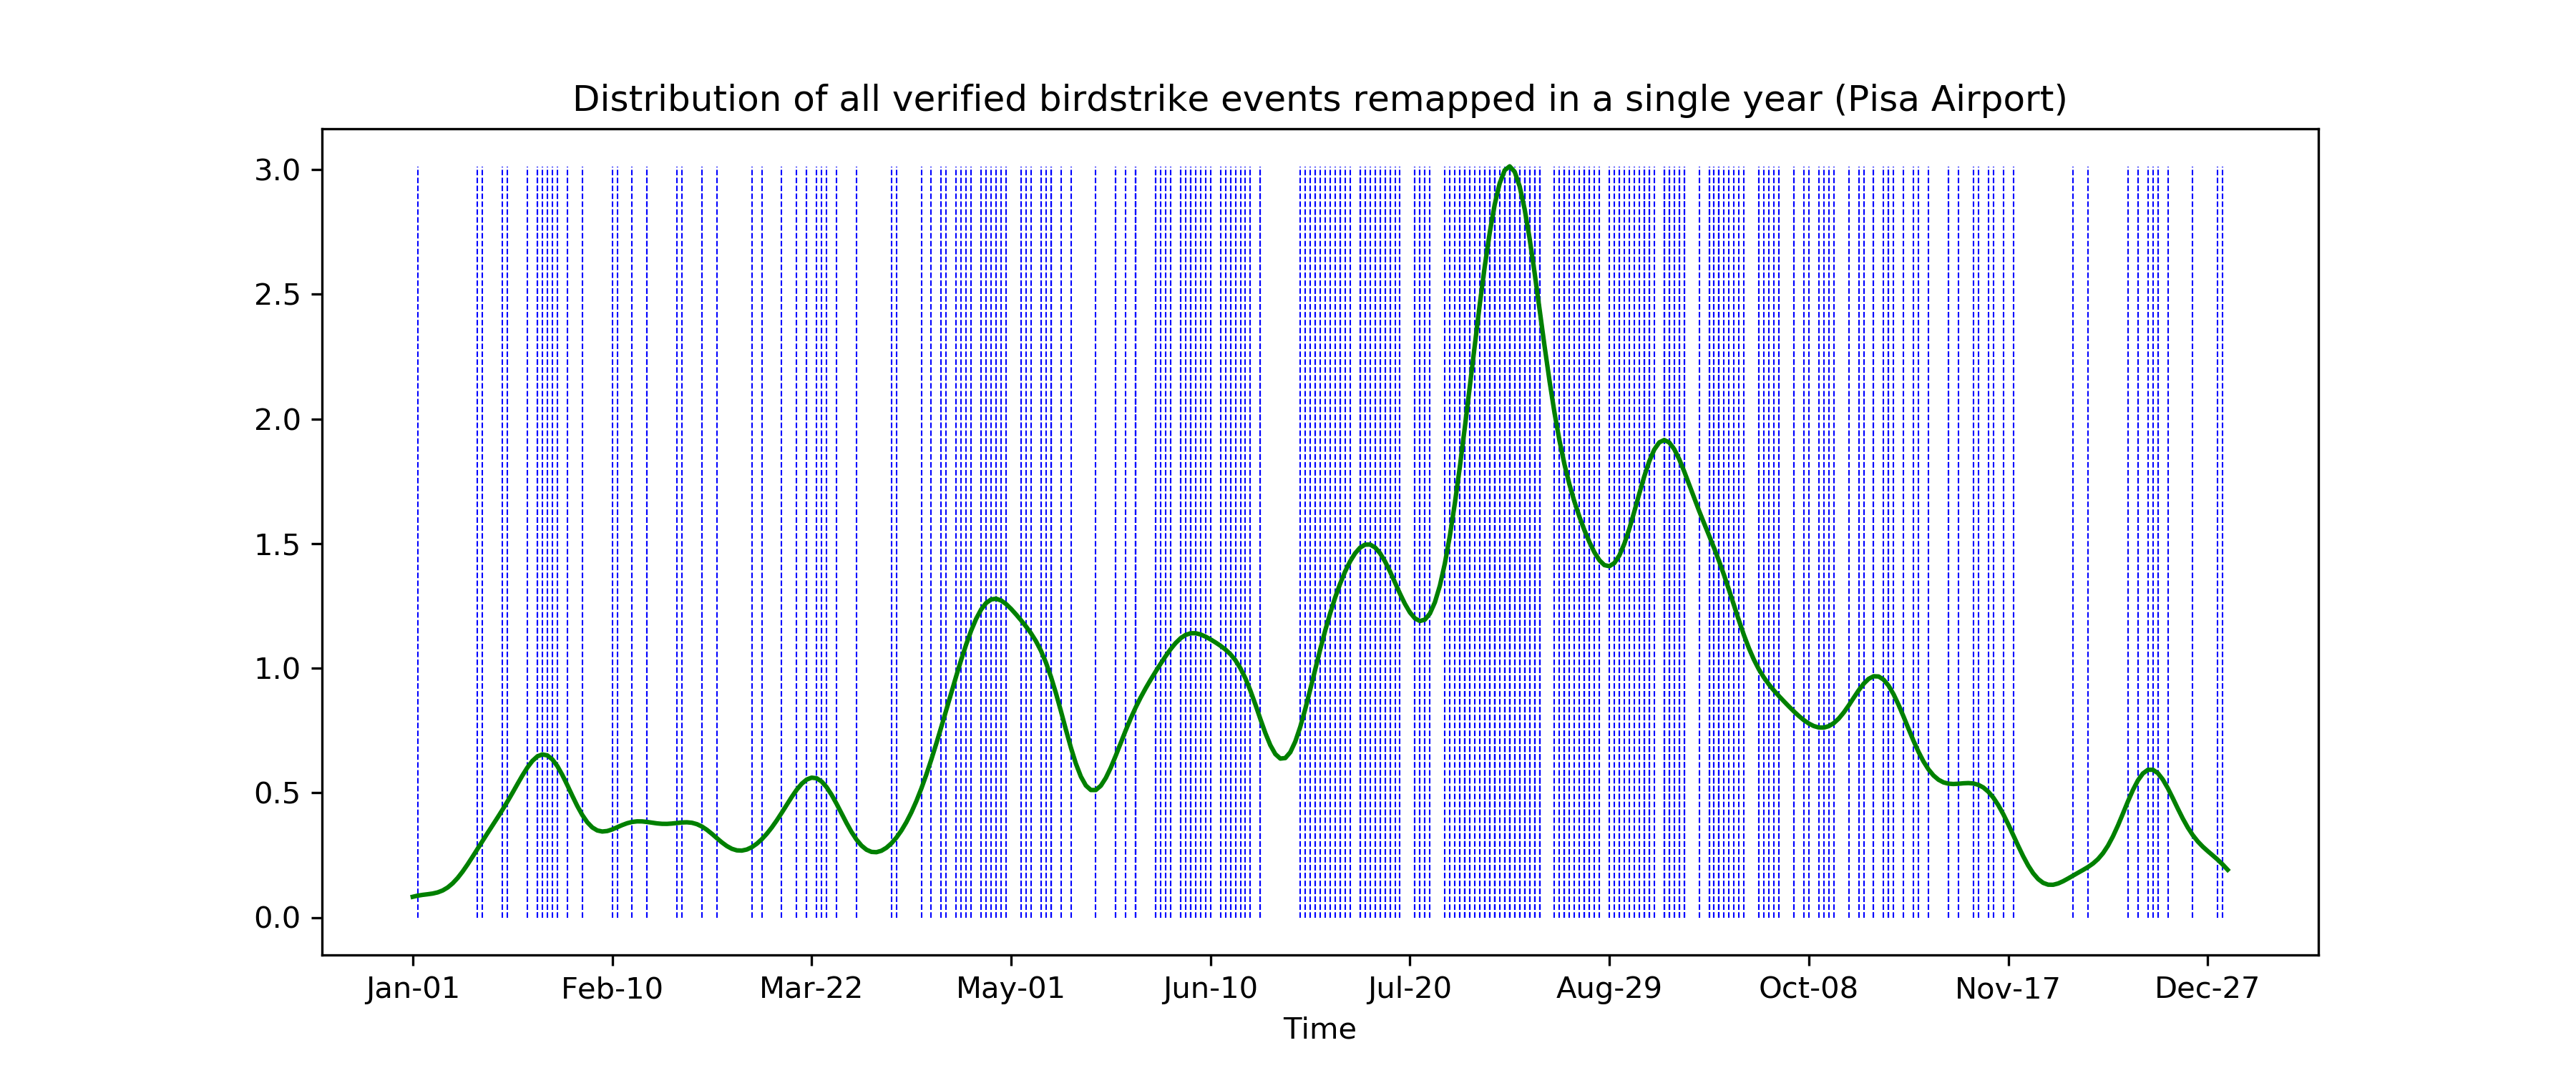
\includegraphics[width=13.8cm]{img/plot_distrib.png}
	\caption{Distribution of all verified birdstrike events remapped in a single year for Pisa Airport. The figure shows how the historical events of birdstrike collected are present all year long but focusing more on a specific period, from June to October indicating a seasonal trend}
	\label{bird_distrib}
\end{figure}
The number of birdstrikes and birdstrikes of the previous year have contributed significantly to the model's performance, considerably increasing the correlation between the new risk index and birdstrike events.

\subsection{Data cleaning}
Once the features to use are chosen it is necessary to clean the data because they are very noisy. This technique consists of detecting and correcting or removing corrupt or inaccurate records from the raw data.
The noisiest features detected were the temperature, direction and intensity of the wind.
These features contained missing, incorrect, and incomplete values.
\begin{itemize}
    \item Temperature: only values in the range of degrees [-30, 50] were kept, the rest were removed.
    \item Wind Intensity: the Beaufort scale \cite{huler2007defining} was used to filter out the values to be removed.
    \item Wind Direction: the values outside the degree range [0, 360] were removed.
\end{itemize}
Only missing and corrupt values have been found in the remaining features to be removed without any special measures.

\subsection{Features setup}\label{feat_setup}
To represent the daily features, frequency histograms have been chosen due to the nature of the available database. The features that follow this representation are:

\begin{itemize}
    \item Sighted species: After the data cleaning 288 species were detected between 2011 and 2019. A histogram for each day is computed from these 288 species.
    \item Meteorological conditions: this is a categorical feature. This can take one of these 7 forms: 'Foschia', 'Molto Nuvoloso', ‘'Nebbia', 'Neve', 'Pioggia', 'Poco Nuvoloso', or 'Sereno'. A histogram from all inspections for each day is computed over these 7 forms.
    \item Temperature: the histogram for each day is computed over 35 temperatures.
    \item Wind Intensity and Wind Direction: the histogram for each day is computed over 50 intensities detected.
    \item Wind Direction: the histogram for each day is computed over 130 directions detected.
    \item Distance to the Track: 384 distances have been detected and the histogram for each day is computed on these detections.
    \item Detection environment: a categorical feature, this can take up to 88 forms and, again, the histogram from all inspections for each day is computed over these 7 forms.
\end{itemize}
Finally, the remaining features (Number of Birdstrikes, Number of Birdstrikes of the Previous Year and Presence of Wet Ground) have been represented by occurrence vectors.
The histograms and occurrence vectors have been normalized with min-max normalization.

\subsection{Ground truth}
The ground truth chosen to train the proposed model comes directly from the actual data of historically occurring birdstrike events.
In particular, it is represented by the number of birdstrikes that occurred on the $K+1$ day following the $k$-day observation window.
This ground truth has been chosen because the goal is to generate a risk index as related as possible to birdstrike events.
The same procedure discussed in \ref{smooth} was used to generate it. A Gaussian filter was applied to smooth the occurrence vector of birdstrike events and finally, it was normalized.
Figure \ref{GT_fig} shows an example of ground truth generated for Florence airport from 2012 to 2018.

\begin{figure}
	\centering
	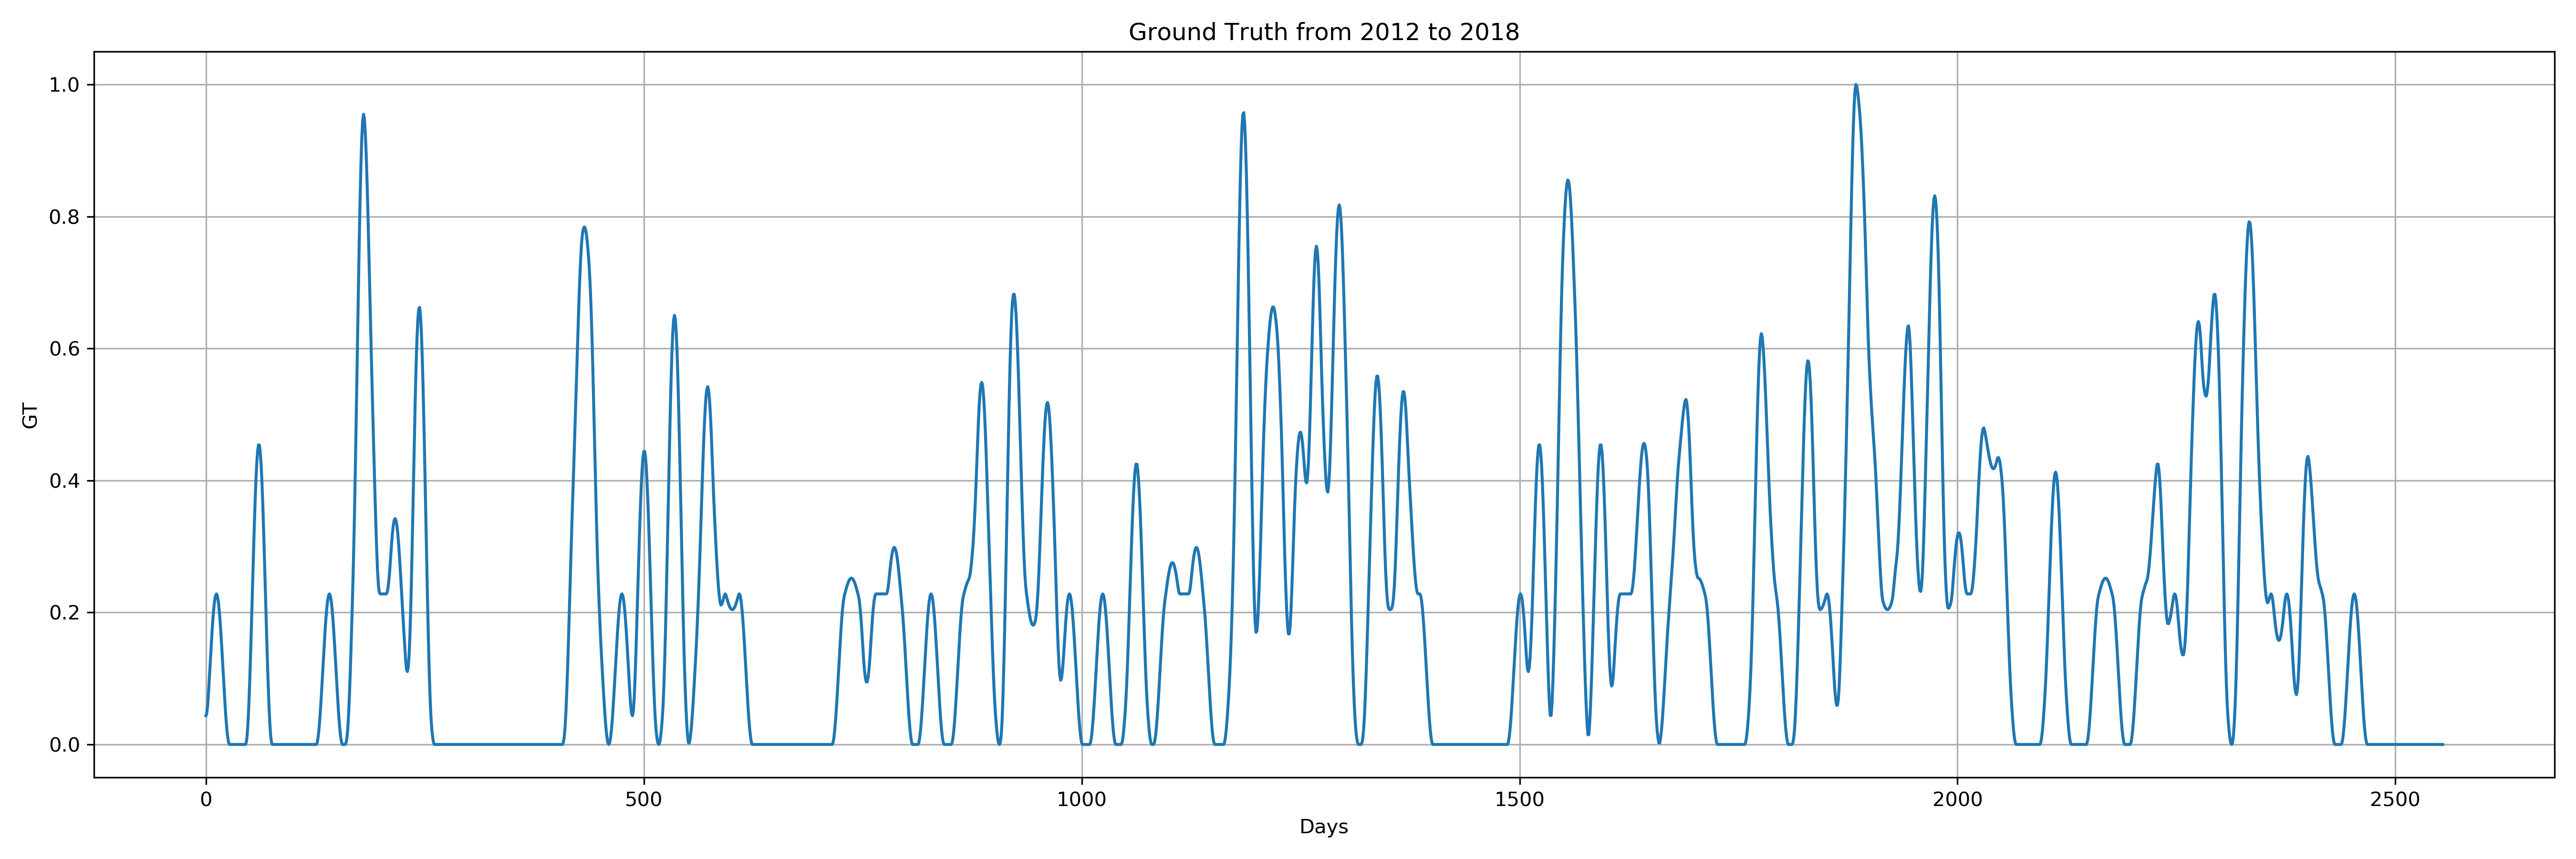
\includegraphics[width=13.2cm]{img/GT.png}
	\caption{The Figure shows an example of Ground truth generated for Florence airport from 2012 to 2018. The risk index provided by the proposed model must be very much related to the ground truth, generated by the historical events of birdstrike.}
	\label{GT_fig}
\end{figure}

\section{Model}\label{model_section}
The proposed model has been implemented using Machine Learning techniques, in particular Neural networks (Deep Learning, \ref{deep}).
Since the goal is to provide a risk value of the $K+1$ day, observing $K$ previous days, the model must work with time series. The model is based on a daily aggregation of factors, i.e. the features selected in \ref{feat_setup}, for generating the new risk-index. 
Features are embedded using a simple and learned non-linear transformation, and these embeddings are then fed into a recurrent neural network that then provides the risk value for the following day. The model uses a type of Recurrent neural network known as LSTM, \ref{LSTM_subs}.
Spearman correlation was used as accuracy to evaluate the model's performance. We did not choose it as a loss function because it is not differentiable and a loss function must be differentiable.
In order to increase the Spearman correlation between the predicted values and the ground truth, the use of multi task learning \cite{1997multitask} was chosen. To apply this approach it was necessary to design the model with the architecture of a Siamese neural network.
In the following subsections the embedding layers and the model architecture will be described.

\subsection{Embeddings}\label{embeddings_section}
A standard technique for Neural networks is to embed data into a higher- (or lower) dimensional space in order to use a learned representation of input data. 
This technique has been useful for our problem. Raw histograms are poor features for direct use in Neural networks and by using learned feature embeddings it was possible to mitigate the problem.

The embeddings size chosen for the features represented by histograms are:

\begin{itemize}
    \item Sighted Species: has been mapped from 288 dimensions down to 256 embedding dimensions.
    \item Meteorological conditions: has been mapped from 7 dimensions (all the possible weather conditions) up to 32 embedding dimensions.
    \item Temperature: has been mapped from 35 dimensions down to 32 embedding dimensions.
    \item Wind intensity: from 50 dimensions down to 16 embedding dimensions.
    \item Wind direction: from 150 dimensions down to 16 embedding dimensions.
    \item Distance to the track: from 384 dimensions down to 256 embedding dimensions.
    \item Detection environment: from 88 dimensions down to 32 embedding dimensions.
\end{itemize}
Then the resulting embeddings were concatenated with the occurrence vectors to form the final feature representation that is used as input to the LSTM layers.

\subsection{Architecture}
As mentioned previously, the core of the model is the LSTM layers and the Siamese architecture was chosen with the aim of increasing the correlation.
The model, shown in Figure \ref{architecture} is composed of two identical branches which share the same weights and architecture.
After extracting the features from the raw data in the database as discussed in section \ref{feat_setup} , the raw histograms have been embedded into embedding layers.
Then the resulting embeddings were concatenated with the occurrence vectors to form the final feature representation.
The final feature has been reshaped. The LSTM layers work with sequences and need to know what input shape they should expect.
The new shape is composed from Batch-size (number of samples that will be propagated through the network), Window (number of the days observed) and final feature.

The reshaped feature is the input for the LSTM layers. Specifically, each branch has 2 LSTM layers that sequentially process two different K-day windows. Finally, a final linear layer for each branch, with the same LSTM output size as input size, provides the risk values for the following day of the window processed.
After the embeddings layers and LSTM layers the ReLU \cite{relu} activation function was applied. And finally after the final layer the Sigmoid \cite{sigmoid} activation function was used.

The model uses a mini-batch size of 64 examples. It has been regularized by applying L2 Regularization \cite{ng2004feature} (with $\lambda = 1\times10^{-3}$), using dropout \cite{srivastava2014dropout} on the LSTM layers of 0.2 and using Adam as the Optimizer \cite{adam}.

\begin{figure}
	\centering
	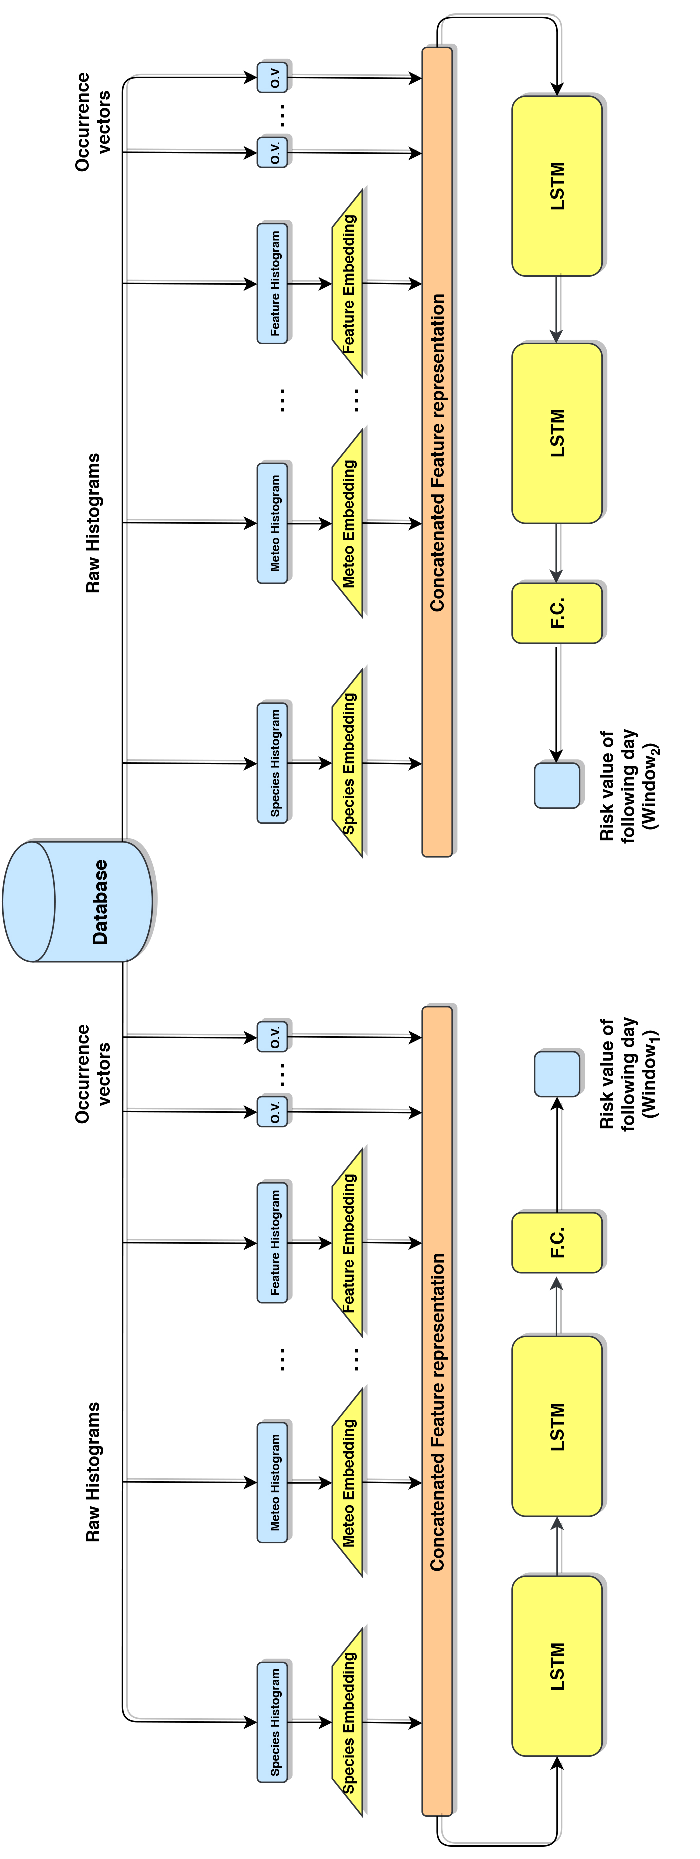
\includegraphics[width=7.3cm]{img/network2.pdf}
	\caption{The Model Architecture. Data extracted from the database are grouped by histograms and occurrence vectors. These histograms and vectors are then processed by learned embeddings (section \ref{embeddings_section}) before finally being sequentially processed by an LSTM which looks at K days of embedded factors before providing a risk-value for the following day.}
	\label{architecture}
\end{figure}

\subsection{Loss function}\label{Loss_function}
As discussed in \ref{model_section}, to improve the model's performance and generate a new risk-index more related to birdstrike events, Multi Task Learning (MTL) was chosen.
MTL help in improving the learning of the model by using the knowledge contained in two specific tasks.
The first task is to provide a risk value of the $K+1$ day, observing $K$ previous days; this is a regression problem.
The second task is to rank two risk values of two different days, i.e. the model tries to learn, given two different observation windows, which of the following two days will have higher risk.

A Custom loss function has been defined to train the model using the 2 tasks.
It takes two arguments:

\begin{itemize}
    \item Mean Absolute Error, or L1 Loss, for the first task, equation \ref{MAE}.
    \item Margin Ranking Loss (MRL), for the second task in equation \ref{MRL}.
\end{itemize}

\begin{equation}\label{MAE}
L_{MAE}(y, \hat y)=\frac{1}{N}\sum_{i=0}^N |y - \hat y|
\end{equation}

\begin{equation}\label{MRL}
L_{MRL}(y, \hat y, z) = \max(0, -z \cdot (y - \hat y) + m)
\end{equation}
where $\hat y$ is the prediction, $y$ is the Ground truth value and $z$ is the target i.e. if $z=1$ then it assumed the first input should be ranked higher (have a larger value) than the second input, and vice-versa for $z=-1$ .

Finally, the final form of the Custom loss of the model is shown in the equation \ref{custom_loss}.

\begin{equation}\label{custom_loss}
\mathcal{L}(L_{MAE}, L_{MRL})= L_{MRL} + \sigma(L_{MAE1} + L_{MAE2})
\end{equation}
where $\sigma$ is a hyperparameter, $L_{MAE1}$ and $L_{MAE2}$ are the L1 loss computed on the two network branches.

\subsubsection{Stabilization of Spearman correlation}
The Custom loss caused an unstable correlation in model training. The accuracy was found to be too sensitive to the variation of epochs, i.e. the correlation of the model would have been too dependent on the stop time.
After an ablation study on $\sigma$, a learning scheduler \cite{2012practical} was identified as a possible solution to the problem.
For some $\sigma$ values improvements were found by lowering the learning rate, and finally using the learning rate scheduler by gradually lowering the learning rate the correlation stabilized.
Specifically, the learning rate scheduler starts from a learning rate of $1 \times 10^{-5}$ and every 200 epochs is multiplied by 0.75, and the best performances were obtained with $\sigma = 0.1$.














\chapter{Experimental results}\label{ch:Ch.5}
This chapter discusses the results achieved by the model described previously in \textit{Chapter \ref{ch:Ch.4}} through the tests performed.
Then a comparison between the proposed model, other techniques used in testing and the $BRI_2$ is shown.
The results include a subset of airports where the accuracy of the model was verified.

\section{Model results}\label{results}
The proposed model has been tested on a subset of airports contained in the available dataset including Florence, Pisa, Bologna, Milan-Malpensa, Milan-Linate, Catania, Brescia, Verona.
An observation window of 15 days was used for the test to provide the model with enough time information. These are very important due to the seasonal trend of birdstrike events. Observations of 15 days showed promising performance on the tests.
The tests were performed inclusively between the year 2012 and 2018. The resulting dataset was split 75\%:
\begin{itemize}
    \item The train-set is composed of 1852 days.
    \item The test-set is formed by 575 days.
\end{itemize}
The model has been trained for 600 epochs. Additional epochs may cause the model to overfit.
The learning rate chosen was $1\times10^{-5}$ and to guarantee the stability of the correlation the learning rate scheduler multiplies it by 0.75 every 200 epochs, as discussed in \ref{Loss_function}.
The Custom loss was set with $\sigma = 0.1$.
The Spearman correlation was chosen to evaluate the model's performance, and quantitative results (correlation) and qualitative results, i.e. the comparison between Ground Truth and the new risk-index, will be shown below.


\begin{figure}
	\centering
	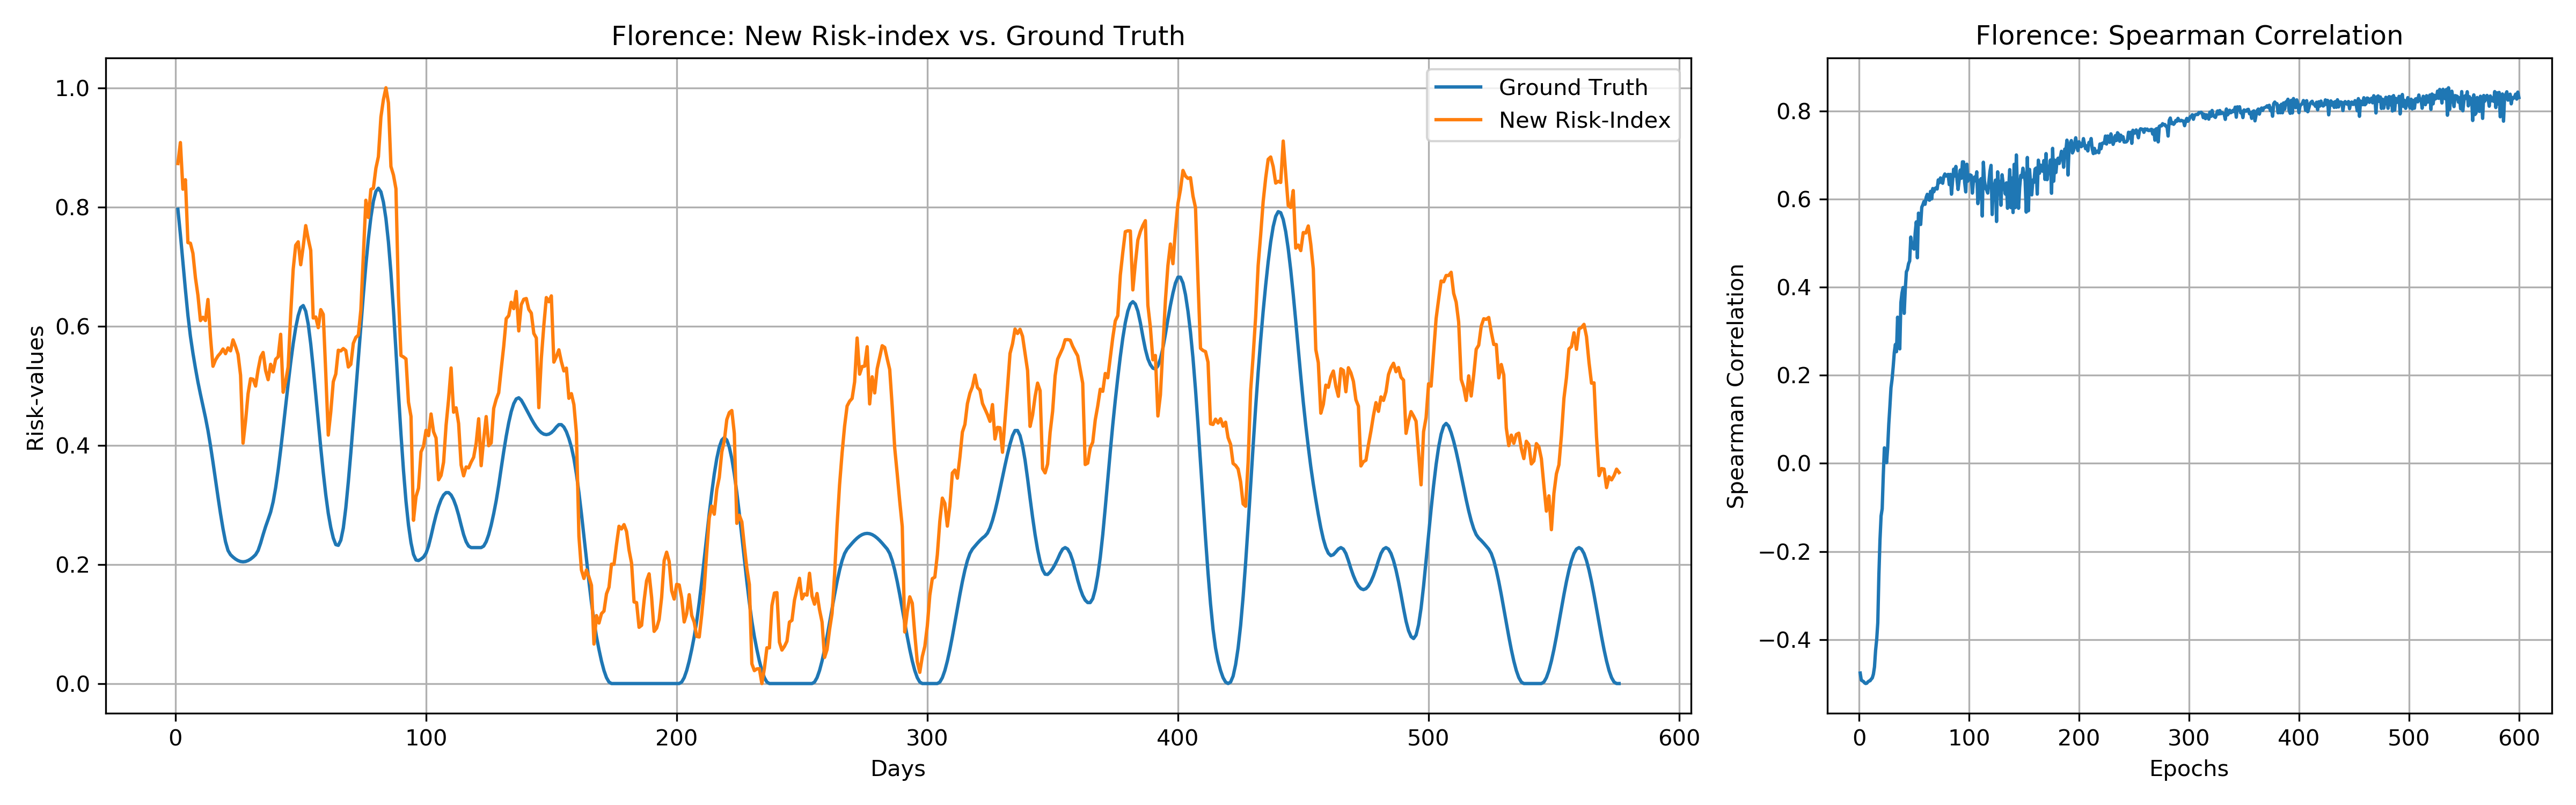
\includegraphics[width=14cm]{img/FI.png}	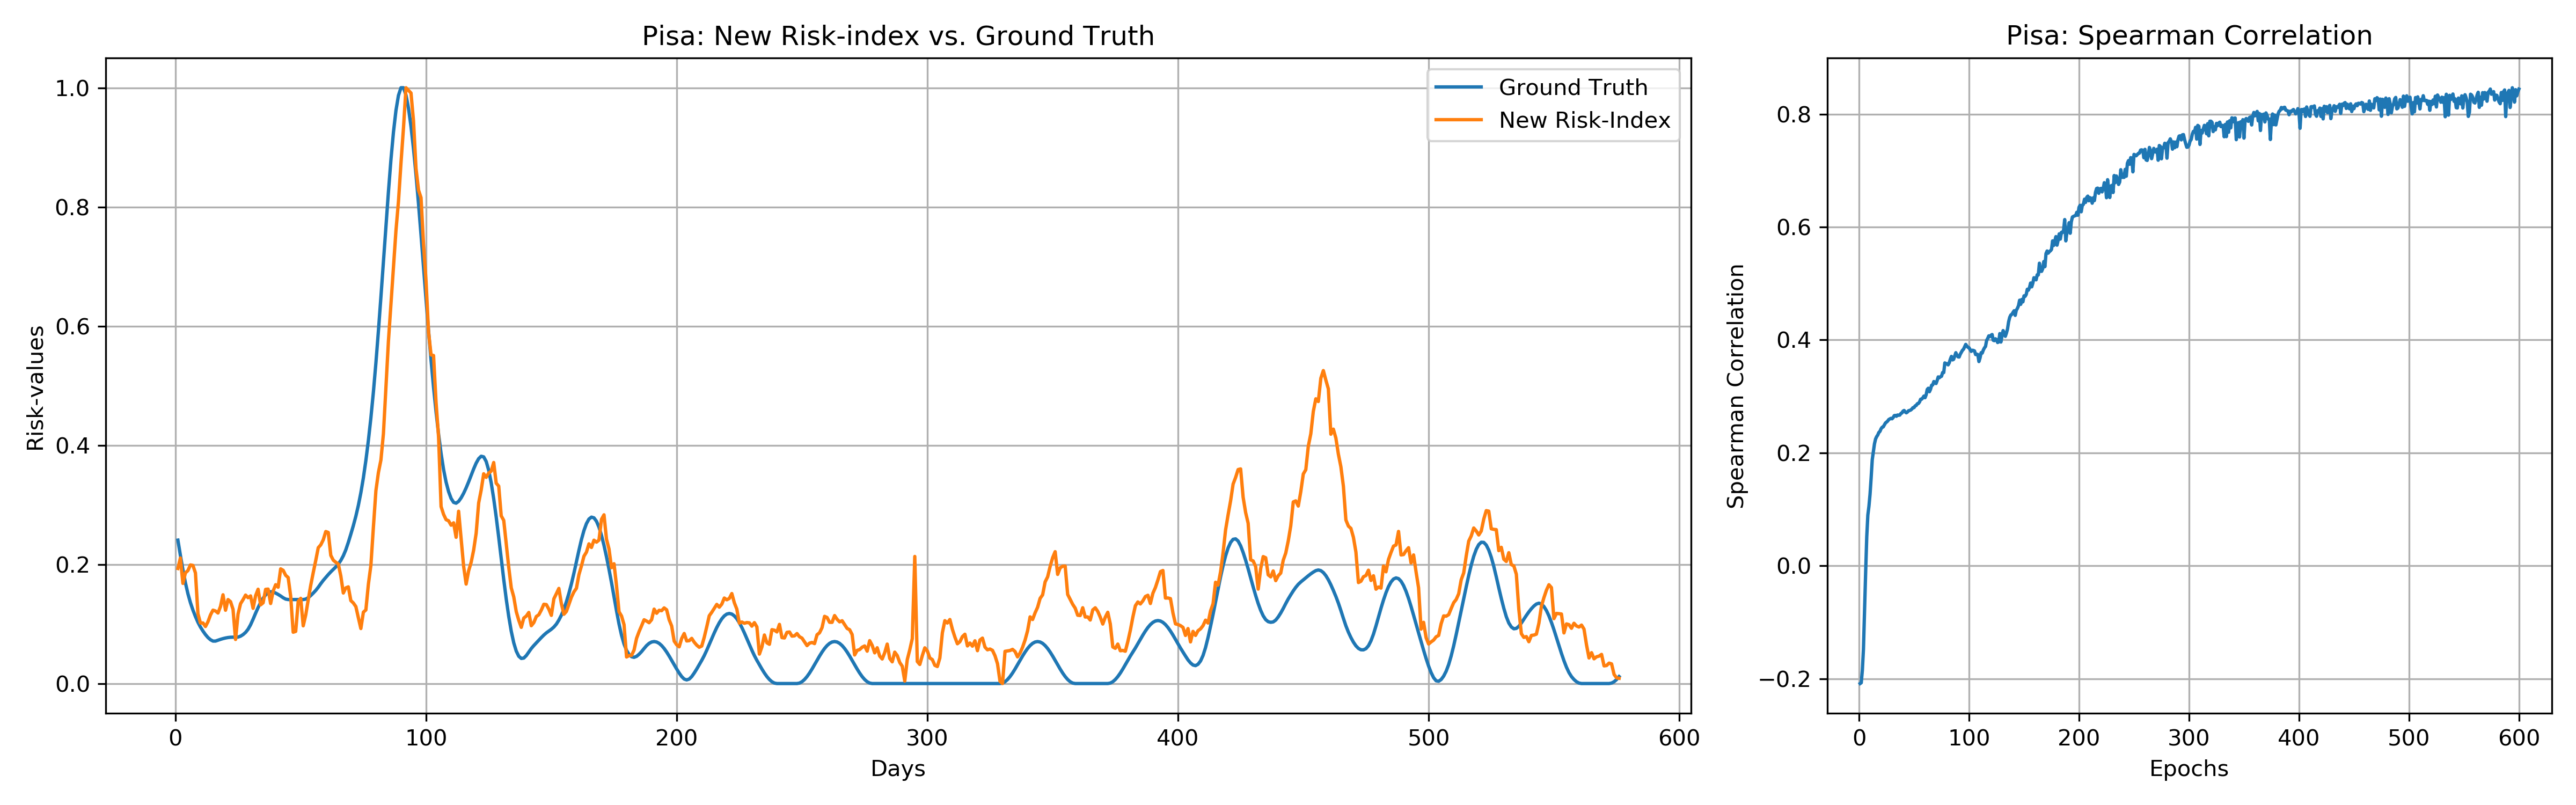
\includegraphics[width=14cm]{img/PSA.png}
	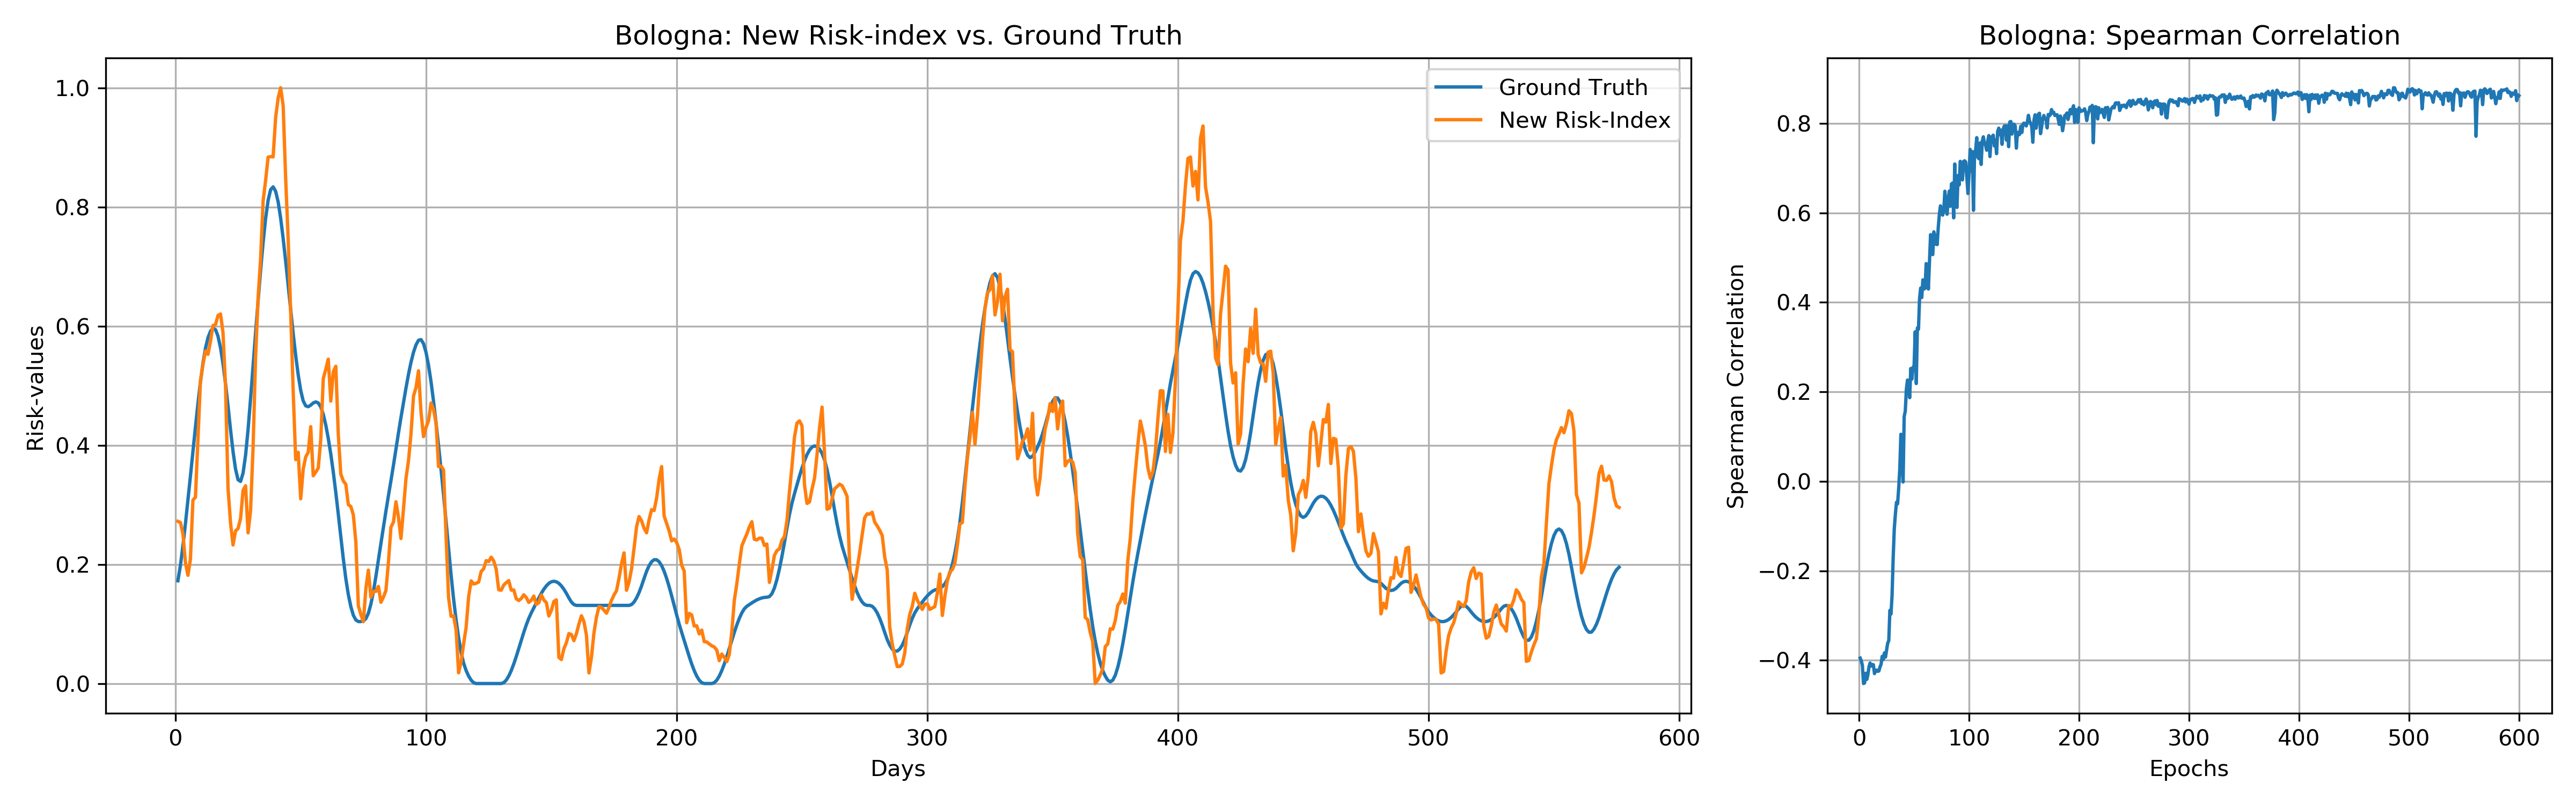
\includegraphics[width=14cm]{img/BO.png}
	\caption{Results for the airports of Florence, Pisa and Bologna. On left the comparison between Ground Truth and the new risk-index, and on right the Spearman correlation. The proposed model is a very accurate risk predictor, the correlation with birdstrike events is high with values of 0.83, 0.84, 0.86.}
	\label{FI_PSA_BO_results}
\end{figure}

\begin{figure}
	\centering
	\includegraphics[width=14cm]{img/malpensa.png}
	\includegraphics[width=14cm]{img/catania.png}
	\includegraphics[width=14cm]{img/verona.png}
	\caption{Results for the airports of Milan-Malpensa, Catania and Verona. On left the comparison between Ground Truth and the new risk-index, and on right the Spearman correlation. The proposed model is a very accurate risk predictor, the correlation with birdstrike events is high with values of 0.82, 0.86, 0.87.}
	\label{MAL_CA_VE_results}
\end{figure}

\begin{figure}
	\centering
	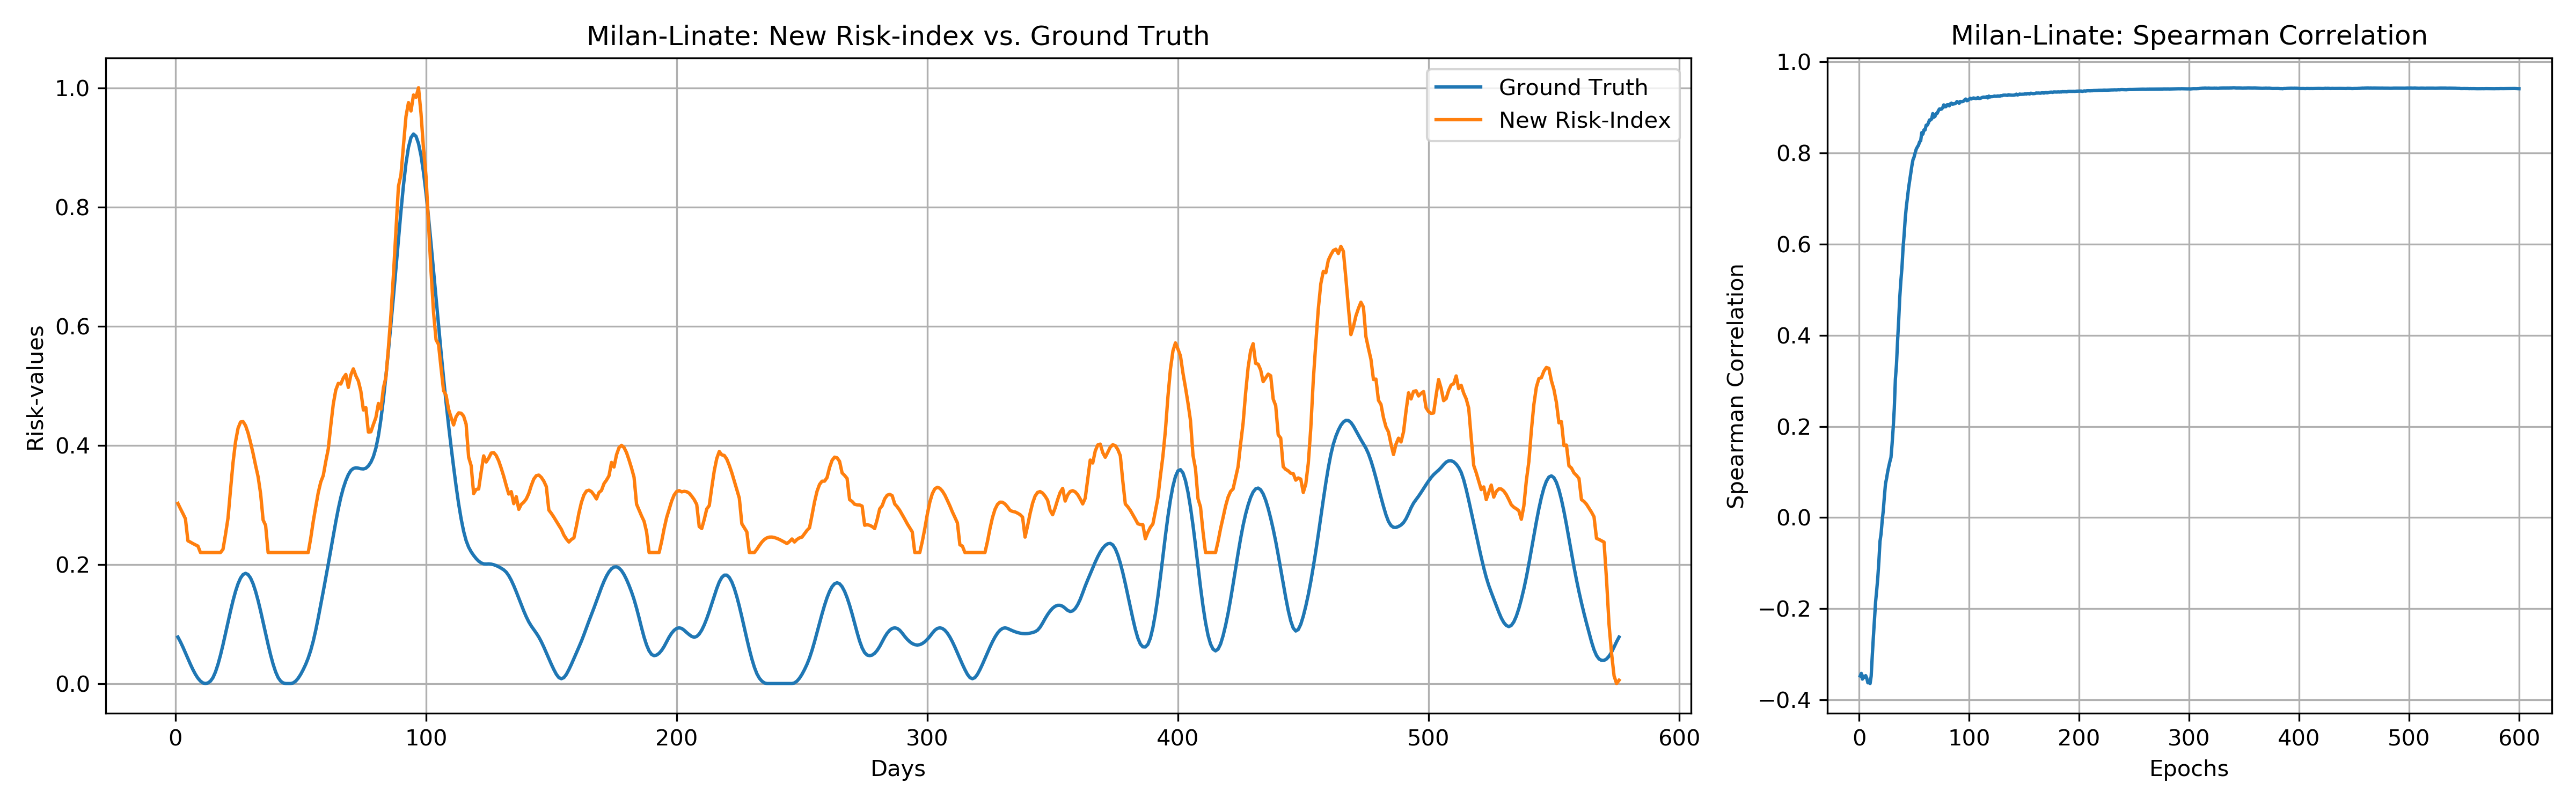
\includegraphics[width=13.8cm]{img/LI.png}
	\caption{Milan-Linate airport results. On left the comparison between Ground Truth and the New Risk-Index, and on right the Spearman correlation.  The proposed model is a very accurate risk predictor, the correlation with birdstrike events is high with a value of 0.94.}
	\label{LI_results}
\end{figure}


The figures \ref{FI_PSA_BO_results}, \ref{MAL_CA_VE_results} and \ref{LI_results} show how the proposed model is able to predict the periods of birdstrike events with very good approximation. The model is able to interpret which are the most dangerous periods and provide a risk value consistent with the events historically occurred.
This is confirmed by the Spearman correlation values for the airports tested.
These values are very promising and indicate an effective correlation between birdstrike events and the new risk-index generated by the model.
Only Brescia Airport did not return good results, with a low correlation.  The data regarding birdstrikes at this airport are insufficient and poorly reported for the training of the model.
In particular, the figures \ref{FI_PSA_BO_results}, \ref{MAL_CA_VE_results} and \ref{LI_results} show on the left the comparison between the Ground Truth and the new risk index, and on the right the Spearman correlation value for each test epoch.
In Table \ref{tab-model_acc} it is possible to observe the results quantitatively for each analyzed airport:

\begin{table}
	\centering
	\scalebox{1.0}{
	\begin{tabular}{@{}ccc@{}}
		\toprule
		Airport & Proposed Model & $BRI_2$ \\ 	\midrule
		Florence & 0.83 & 0.17\\
		Pisa & 0.84 & 0.74\\
		Bologna & 0.86 & 0.26\\
		Milan-Malpensa &  0.82 & -0.14\\
		Milan-Linate &  0.94 & -0.28\\
		Verona & 0.87 & 0.6\\
	    Catania & 0.86 & 0.49\\
	    Brescia & -0.2 & 0.31\\    \bottomrule
	\end{tabular}}
	\caption{Proposed Model accuracy (Spearman correlation) against the results obtained with $BRI_2$.}
	\label{tab-model_acc}
\end{table}

\section{Results comparison}
The results of the proposed model have been presented in the previous section.
Other models were previously tested as possible candidates to solve the task. These models differ in architecture or are variants of the model already described.
The results of the model must also be compared with $BRI_2$. This comparison is of relevant importance because the goal of the model is to improve the Spearman correlation between $BRI_2$ and birdstrike events. 
The other models evaluated and tested are:

\begin{itemize}
    \item $BRI_2$: the current risk index adopted in Italian airports
    \item LSTM: first appreciable results obtained with Machine Learning techniques on which the following choices were based.
    \item Siamese-LSTM with Custom loss, presented in \ref{Loss_function}, learning rate = $1\times10^{-4}$: first attempt to introduce margin ranking loss to increase the accuracy achieved by the previous model.
    \item Siamese-LSTM with Custom loss, learning rate = $1\times10^{-5}$: model tested to stabilize the Spearman correlation.
\end{itemize}

The Figure \ref{comparison1} shows the comparison of the results of the tested models.
The comparison has been made for the subset of airports that have been analysed. For each airport the Spearman correlation value found with the tests executed for the evaluated models specified above are shown.
It is important to remember that the correlation values of LSTM, Siamese-LSTM(learning rate = $1\times10^{-4}$) and Siamese-LSTM(learning rate = $1\times10^{-5}$) are unstable as discussed in \ref{MRL}.
The comparison shows that the proposed model achieves a higher correlation than the other models tested.
In particular, the most significant comparison is with the $BRI_2$. The proposed model has a better performance than the $BRI_2$ with the exception of Brescia but as discussed in \ref{results} the available birdstrike data are not sufficient to train the model.

The results shown in this chapter are encouraging. The next chapter \textit{Chapter \ref{ch:Ch.6}} will discuss the goals achieved given these results, their importance and the improvements achieved.

\begin{figure}
	\centering
	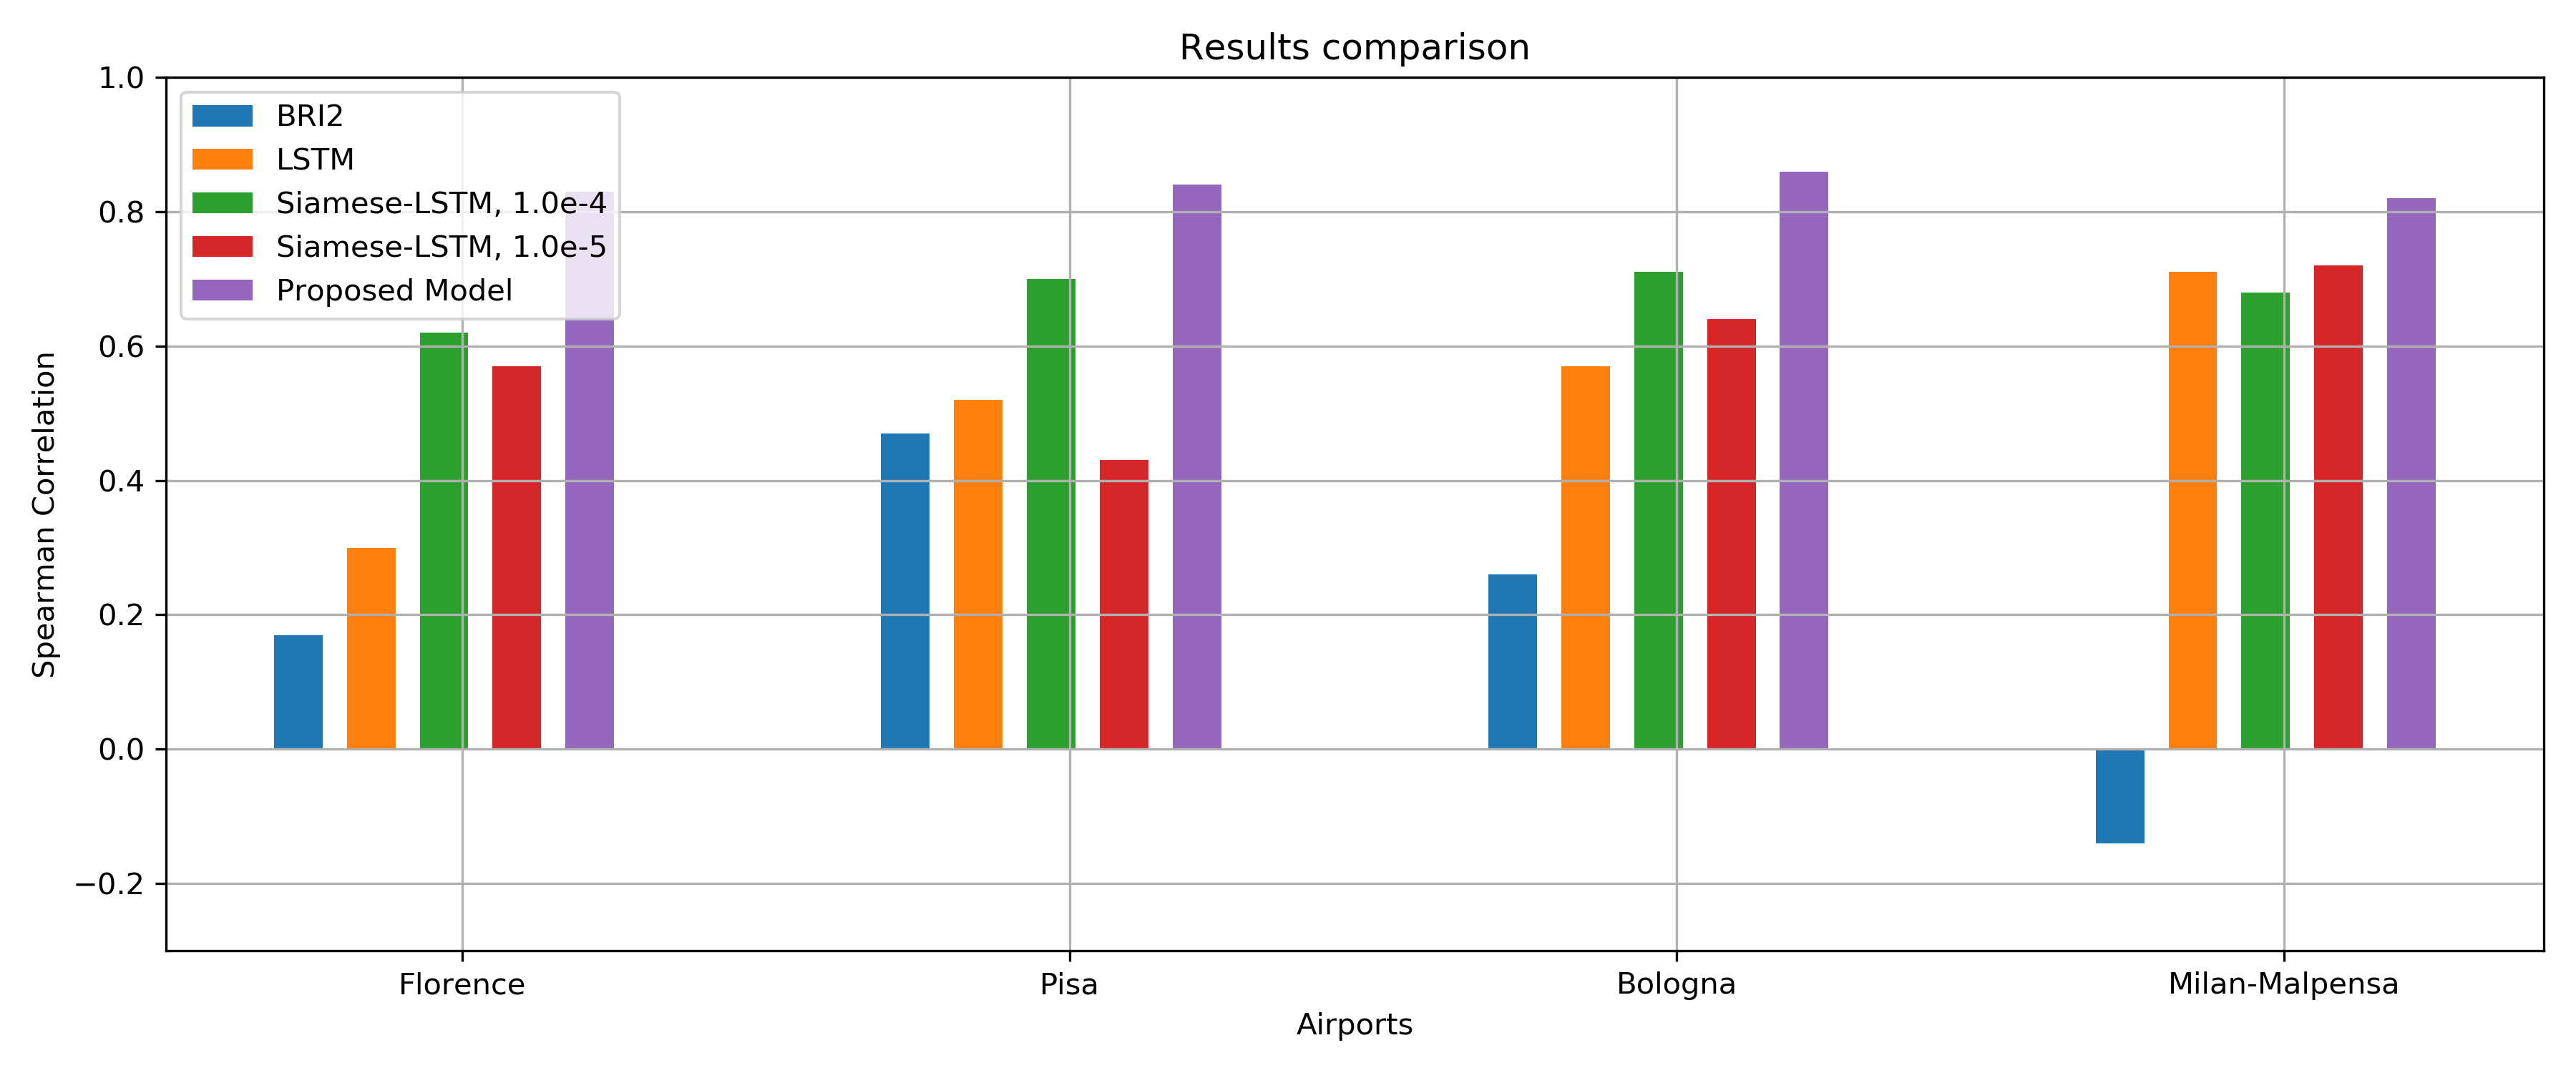
\includegraphics[width=13.8cm]{img/comparison1.png}
	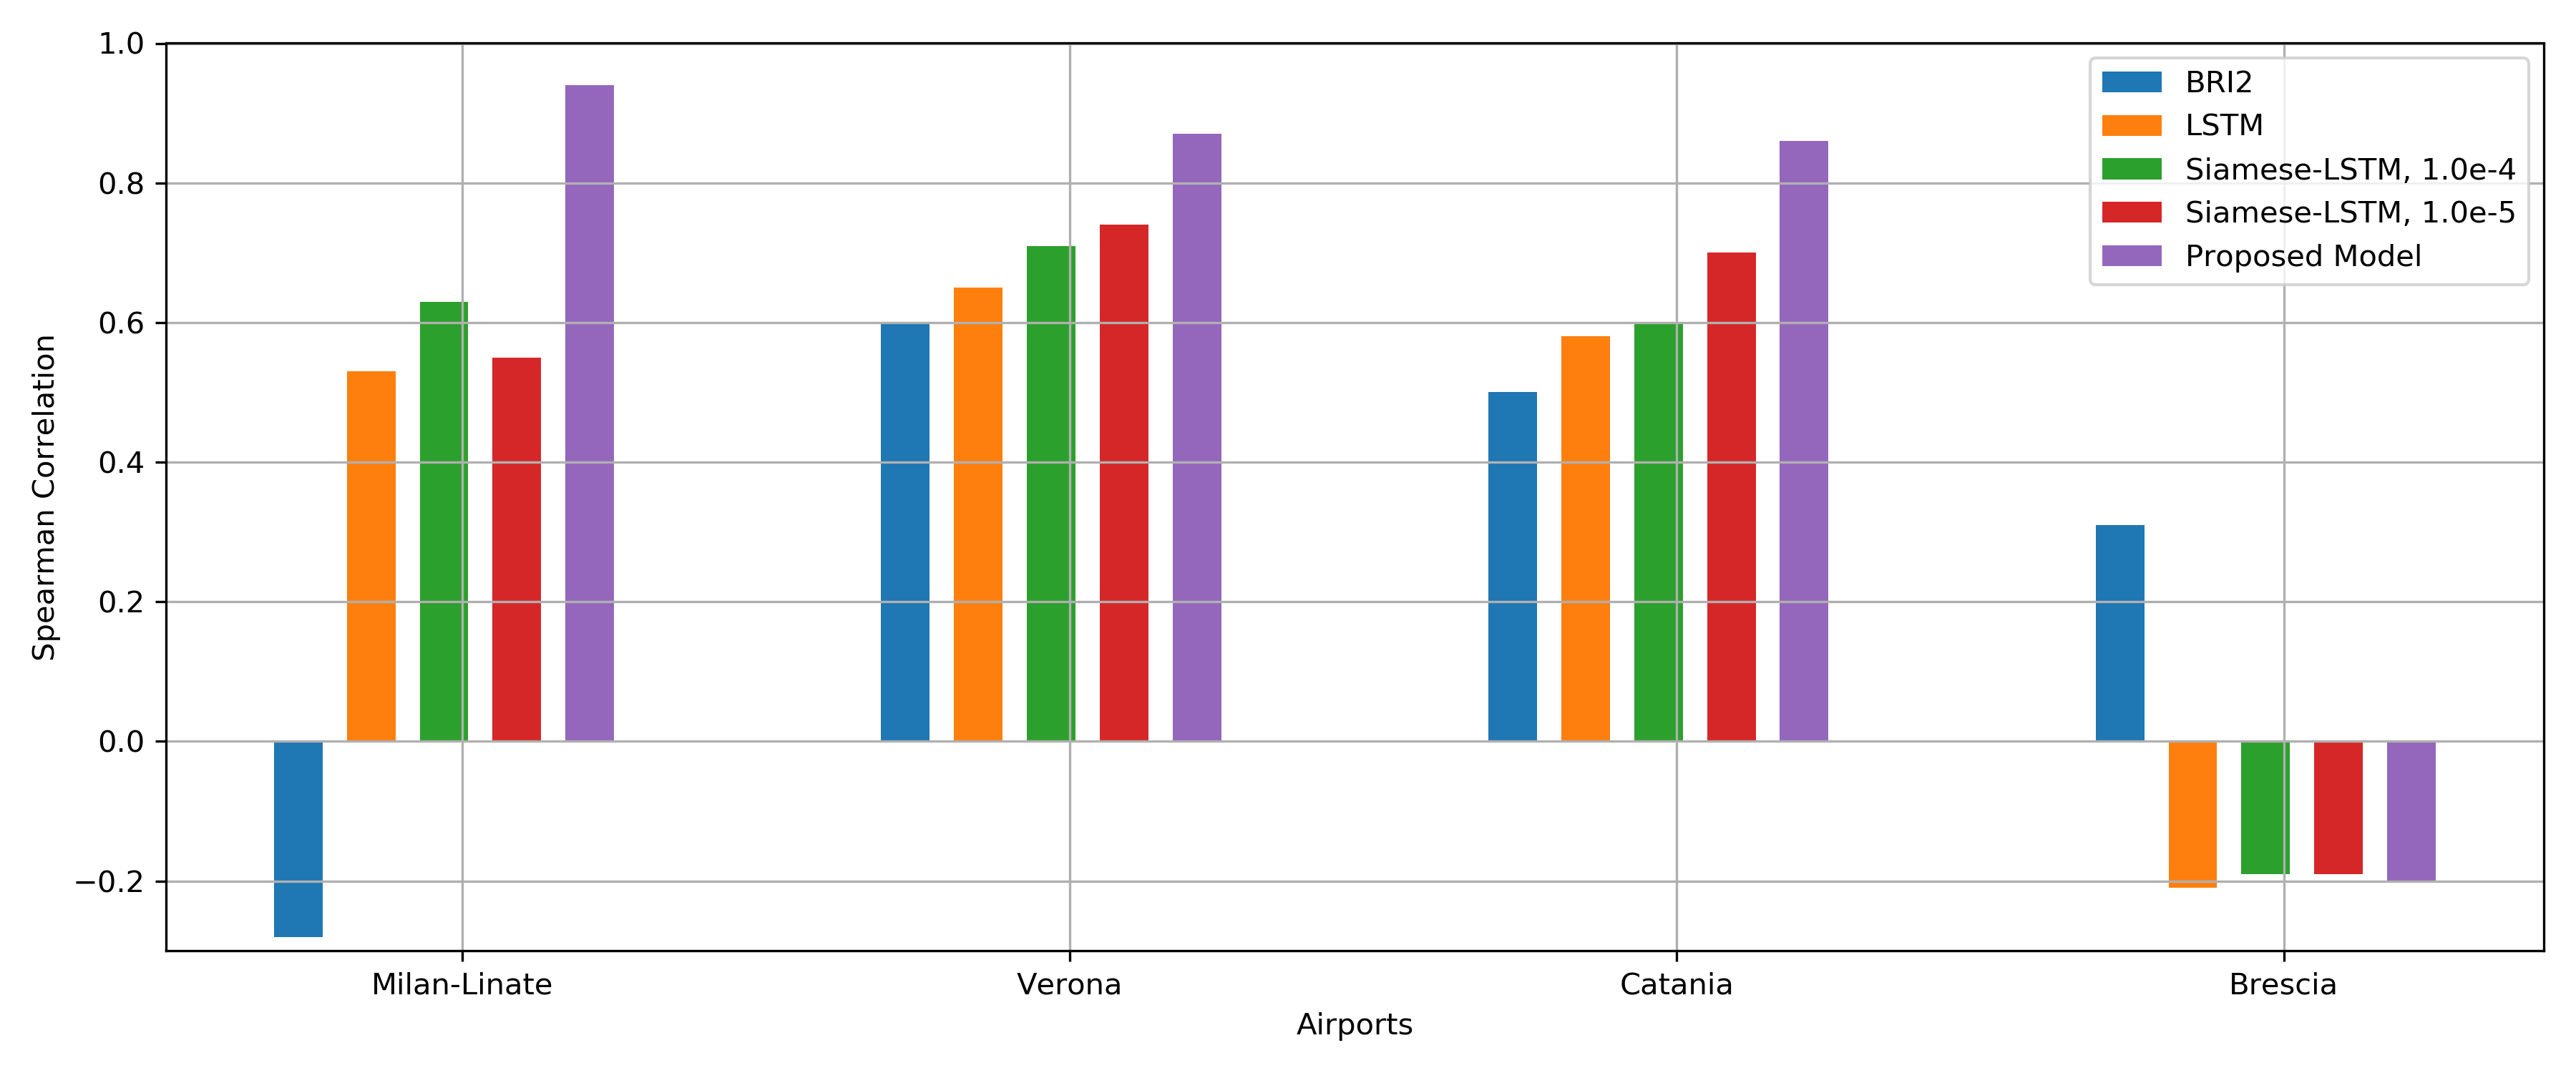
\includegraphics[width=13.8cm]{img/comparison2.png}
	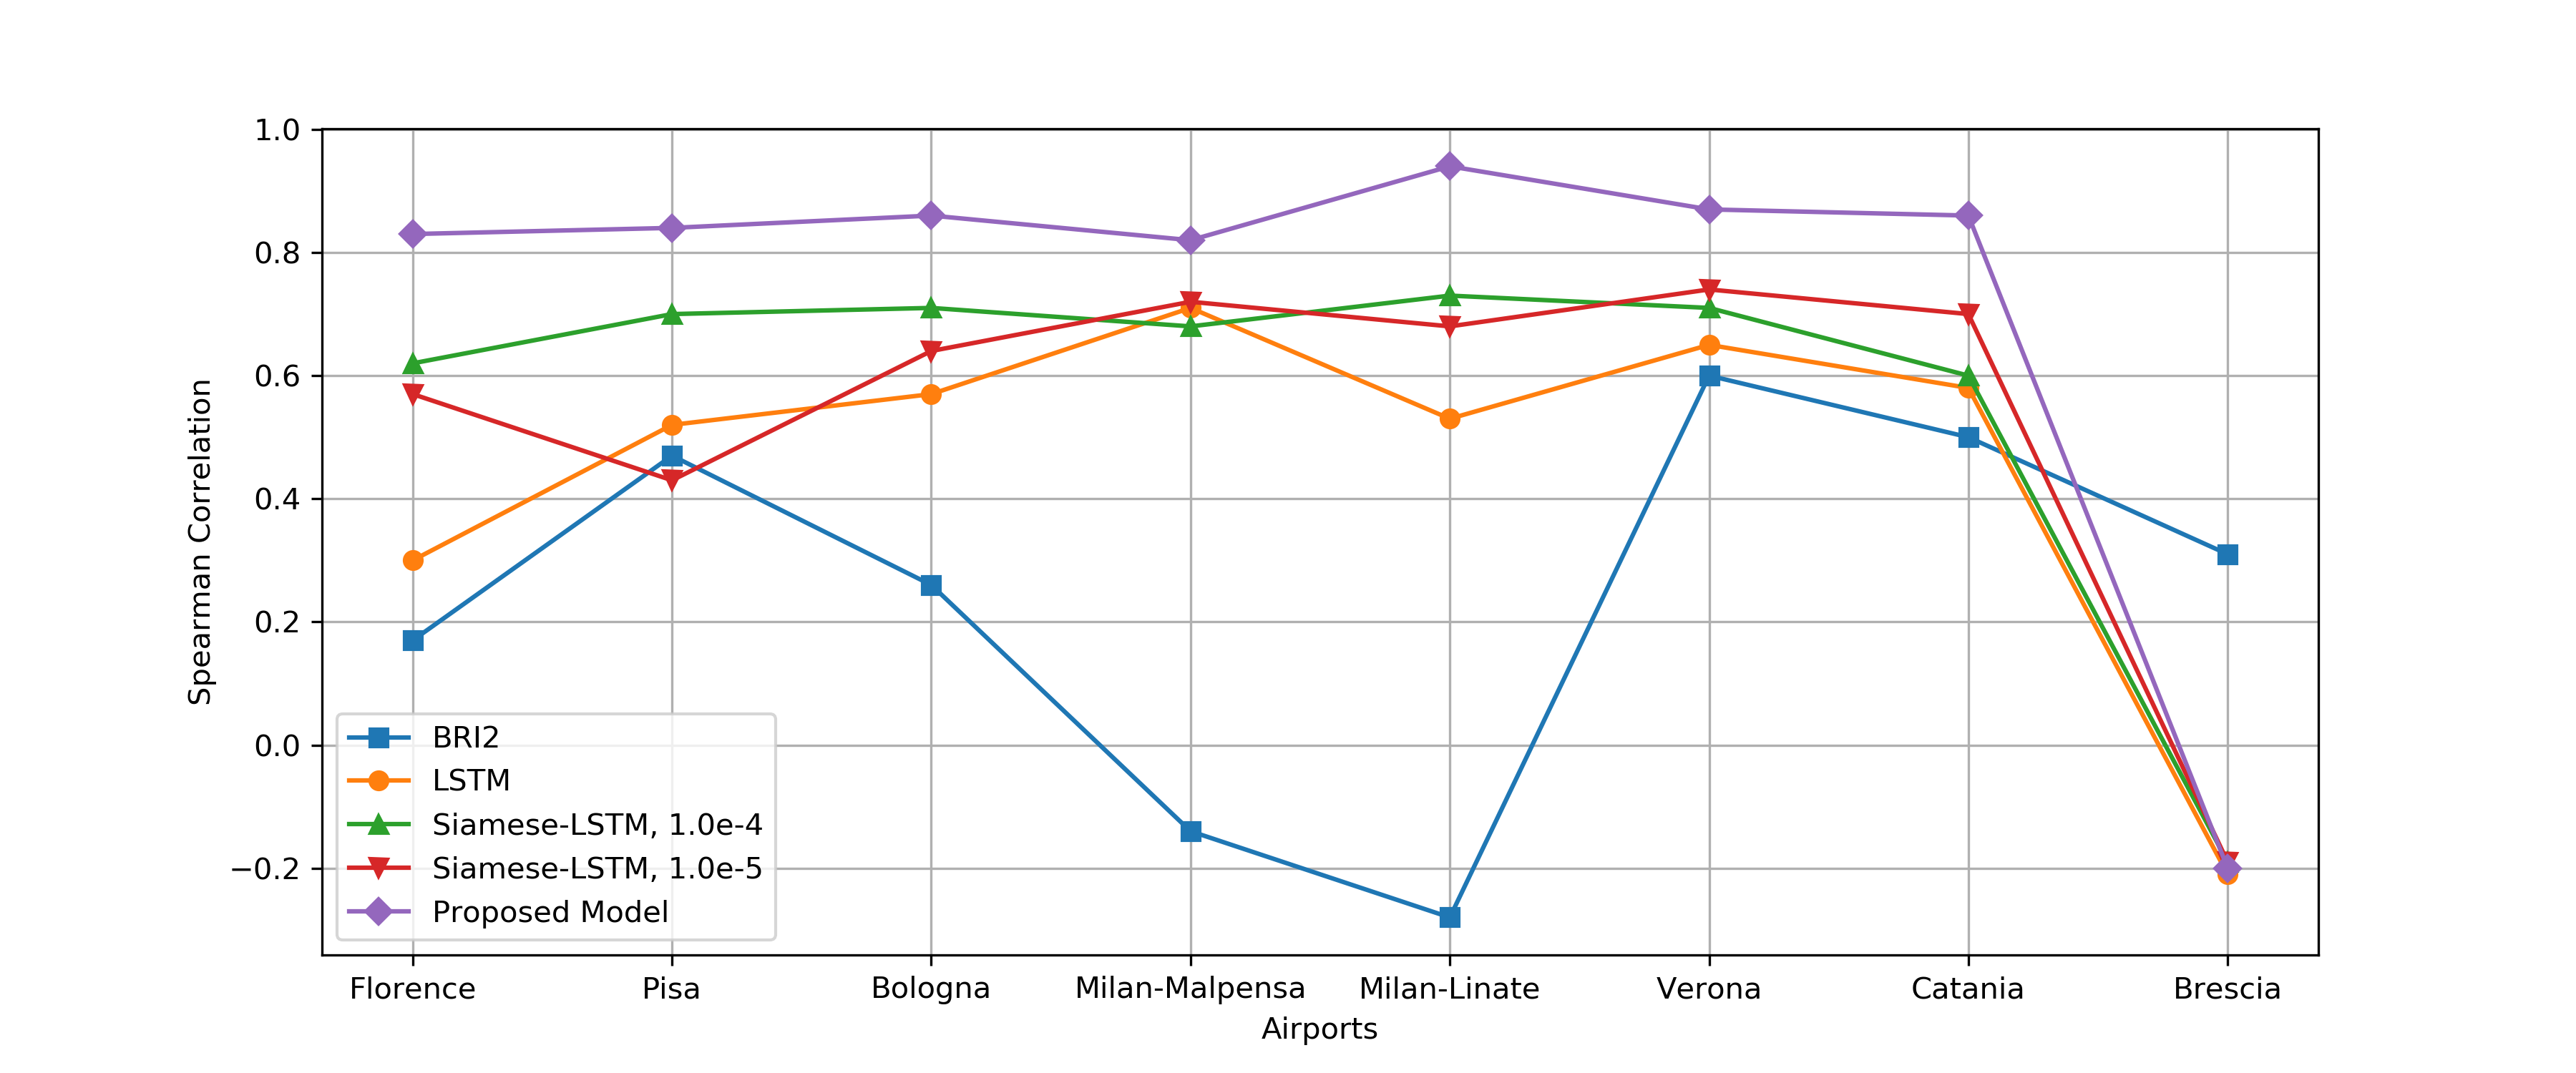
\includegraphics[width=14cm]{img/comparison3_2.png}
	\caption{Models results comparison for Florence, Pisa, Bologna, Milan-Malpensa, Milan-Linate, Verona, Catania and Brescia airports. The figure illustrates how the proposed model shows better performance than the $BRI_2$ and is the data-driven model most related to the birdstrike events collected.}
	\label{comparison1}
\end{figure}

\chapter{Conclusions}\label{ch:Ch.6}
In the previous chapter the results obtained in the tests performed for each airport analysed were shown. This chapter discusses the goals and improvements achieved by the proposed model by comparing the new risk-index with $BRI_2$. 
Finally, some possible future directions will be proposed for the improvement of the implemented model.

\section{Goals and improvements achieved}
Birdstrike events are a growing phenomenon due to the increase in flights over the years. It is very important to prevent these events for the safety of passengers but also to reduce repair costs and losses caused by delays.

The main goal of this work has been to generate a risk index able to detect high-risk periods in order to prevent these events. 
This type of task is not trivial, it is closely related to the biology, habits and seasonality of the species that populate a specific airport.

A model that solves this task must know this information as variables and solve a time series forecasting the problem.
Especially the implemented model must have a high correlation with the birdstrike events that historically occurred to evaluate it's goodness and higher than the one shown by $BRI_2$.
The results shown in \textit{Chapter \ref{ch:Ch.5}} are very encouraging.
A very good correlation value with birdstrike events has been achieved for a subset of selected airports and the model is able to identify the most dangerous periods and a reliable predictor of risk.

Another important achievement of the new index is to provide a daily risk value, in particular for the day after the observation window. The current risk index, $BRI_2$, provides the monthly danger value but calculated at the end of the month.
So the model implemented on a daily basis offers a tool that can be better to prevent birdstrike events in a timely manner and optimize prevention costs.

In addition to the monthly basis of $BRI_2$, the analysis done reveals other important limitations:

\begin{itemize}
    \item $BRI_2$ tends to be more insensitive to sightings over the years and how this is reflected in the calculated value.
    \item Creates a ranking of the most dangerous species by counting birdstrike events over the years and keeping their memory.
    
    This means that sightings can be influenced by birdstrike events that occurred many years before and that the risk value is more dependent on the historical rank of the species rather than how many elements were sighted at that time.
    \item The poor correlation of $BRI_2$ with historical bridstrike events, even some airports have revealed correlations with a negative value. 
\end{itemize}


The model developed in this work is not affected by these problems and is proposed as a reliable predictor of risk showing a strong correlation with birdstrike events. 
Finally, the range of risk values between 0 and 1 make the index more interpretable than the $BRI_2$.


\section{Future directions}
The achievements of this work and the encouraging results suggest some possible future developments and directions that can be explored.
Extending the subset of airports on which to test the model could be a first step in continuing the analysis started by this thesis' work.
Adding the number of flights per day as a feature to the model could also increase accuracy. At the moment this has not been possible because only the number of flights per month is reported in the available database. Entering an average of daily flights (i.e. future based data) could have incorrectly altered the model's performance. 

Other possible future developments could bring small changes to the implemented model pipeline or different untested architectures with the aim of increasing performance.
Finally, it would be interesting to try to train the model with data of several airports at the same time, choosing airports with similar characteristics e.g. type of species sighted, number of flights and geographical area.

\addcontentsline{toc}{chapter}{Appendix}
\chapter*{Appendix}
\markboth{Appendix}{Appendix}
\markright{Appendix}

\section*{Wildlife Strike Risk Index}
In this thesis work a further model proposed by BirdControl Italy S.r.l. has been implemented.
This model, the Wildlife Strike Risk Index ($WRI$), has been proposed to replace the current $BRI_2$ with the purpose of:

\begin{itemize}
    \item Simplicity and clarity of calculation
    \item Objectivity and standardization
    \item Independence from daily monitoring of fauna
    \item Definition of an objective attention threshold
\end{itemize}
The $WRI$ has been defined on the basis of the following 5 components:

\begin{itemize}
    \item $C1$. Ratio between the Wildlife Strike ($WS$) events and number of movements
    \item $C2$. Species involved in wildlife strikes 
    \item $C3$. No. Individuals involved for $WS$
    \item $C4$. Effect on flight and affected part of the aircraft
    \item $C5$. Efficiency monitoring strategy
\end{itemize}
Calculated the 5 components, you can estimate the $WRI$ with the following formula in equation \ref{WRI_Formula} :

\begin{equation}\label{WRI_Formula}
WRI= \frac{\sum_{i=1}^5 C_{i}}{100}
\end{equation}

\subsubsection{C1}

This component is a measure of risk frequency, and is calculated by comparing the number of wildlife strike events with the number of movements ($mov$) within the airport during the month.
An airport that records 20 or more $WS$ for every 1000 movements (2\% or more) is assigned a maximum value of 25 (this ensures that the $WRI$ takes a maximum value of 1), therefore:

\begin{equation}\label{to_c1_1}
20 : 1000 = 25 : X \\
\end{equation}
\begin{equation}\label{to_c1_2}
X = (1000 \cdot 25)/20 = 1250
\end{equation}
Finally, given the equations \ref{to_c1_1} and \ref{to_c1_2}, $C1$ is computed with the following formula in equation \ref{C1}:

\begin{equation}\label{C1}
C1 = \frac{\frac{\mathrm{WS}}{\mathrm{month}*1250}}{\mathrm{mov}/\mathrm{month}}
\end{equation}

\subsubsection{C2}
This component is a measure of the severity of the risk, and is calculated on the basis of a heuristic matrix \cite{allan2006heuristic}, associating a value between 1 and 25 to the species involved in each event.

\subsubsection{C3}
This component is a measure of the severity of the risk, and is calculated by associating a value (from 1 to 5) depending on the number of individuals involved in a wildlife strike event, shown in the Table \ref{tab-c3}.

\begin{table}
	\centering
	\scalebox{1}{
	\begin{tabular}{@{}ccc@{}}
		\toprule
		Number of Animals Involved & Severity of the Risk \\	\midrule
		1 & 1 \\
		From 2 to 10 & 2 \\
		From 11 to 100 & 3\\
		$>$ 100 &  5 \\	\bottomrule
	\end{tabular}}
	\caption{$C3$: measure of the severity of the risk. The table lists in ascending order the hazard values attributed to the number of animals involved in wildlife strike events.}
	\label{tab-c3}
\end{table}

\subsubsection{C4}
This component is a measure of the severity of the risk whose values range from 4.3 to 30 depending on the severity of the $EOF$.
In particular, in case the aircraft is hit and/or damaged the $C4$ value is doubled and in case of a catastrophic event, the $WRI$ value related to that event shall be set to the default value1.
The Table \ref{tab-EOF_wri} show the $EOF$ values:

\subsubsection{C5}

This component is a measure of risk frequency, and is calculated based on the number of unscheduled wildlife strike inspections ($UI$) at the individual airport.
An airport that records 60 or more $UI$ per month has a maximum value of 15 (this ensures that the $WRI$ is at a maximum value of 1), therefore:

\begin{equation}\label{to_c5_1}
60 : 15 = \mathrm{UI} : X
\end{equation}
\begin{equation}\label{to_c5_2}
 X = \frac{15 \cdot \mathrm{UI}}{60}
\end{equation}
Finally, given the equations \ref{to_c5_1} and \ref{to_c5_2}, $C5$ is computed with the following formula in equation \ref{C5}:

\begin{equation}\label{C5}
C5 = \frac{\mathrm{UI} \cdot 15}{60}
\end{equation}

\begin{table}
	\centering
	\scalebox{1}{
	\begin{tabular}{@{}ccc@{}}
		\toprule
		EOF Value & Description \\	\midrule
		4.3 & None \\
		5 & Aborted take-off, delay \\
		6 & Precautionary landing \\
		7.5 &  Engine(s) shutdown \\
		10 & Forced landing \\	
		15 & Visual obstruction \\	
		- & Catastrofic effect \\	\bottomrule
	\end{tabular}}
	\caption{Categories of the Effect On Flight ($EOF$) provoked by wildlife strike events. The table lists in ascending order the values attributed to damage caused by wildlife events.}
	\label{tab-EOF_wri}
\end{table}

By summing up the scores for the five variables presented, the $WRI$ is obtained (eq. \ref{WRI_Formula}). The value is divided by 100, resulting in a value between 0 and 1.
The weighted arithmetic mean of the events recorded in a month gives the monthly $WRI$.
Similarly, the weighted arithmetic mean of the events recorded in a year gives the annual $WRI$.

This model was developed and tested on a subset of airports.
Two main problems were detected:
\begin{itemize}
    \item the first problem is the poor correlation of the $WRI$ with historical birdstrike events,
    \item the second problem is the low risk values that the $WRI$ provides over many years of computing, failing to report the real periods of danger.
\end{itemize}
From a first analysis the $WRI$ is not an accurate risk index and a reliable risk predictor, having in common the poor correlation with birdstrike events as the $BRI_2$ showed. 



\addcontentsline{toc}{chapter}{Bibliography}
\printbibliography
\end{document}